\documentclass{uscthesis}

%%%%%%%%%%%%%%%%%%%%%%%%%%%%%%%%%%%%%%%%%%
%%% Options include: [forbinding], which produces 
%%% an alternative title page and an appropriate
%%% binding margin,  [honors] for Honors College theses,
%%% and [durt] for undergraduate thesis submitted as part
%%% part of the distinction in mathematics program.
%%%%%%%%%%%%%%%%%%%%%%%%%%%%%%%%%%%%%%%%%%

%%%%%%%%%%%%%%%%%%%%%%%%%%%%%%%%%%%%%%%%%%
%%  LaTeX Preamble
%%%%%%%%%%%%%%%%%%%%%%%%%%%%%%%%%%%%%%%%%%

%%%%%%%%%%%%%%%%%%%%%%%%%%%%%%%%%%%%%%%%%%
%% You should include above
%% any LaTeX packages that you need.  Most packages should work 
%% with this documentclass.
%%%%%%%%%%%%%%%%%%%%%%%%%%%%%%%%%%%%%%%%%
\usepackage[backend=bibtex, style=uscnumeric,sortcites=true]{biblatex}
%\usepackage[author-year]{uscamsrefs}
\bibliography{references}

%%%%%%%%%%%%%%%%%%%%%%%%%%%%%%%%%%%%%%%%
%% The lines above specify a BibTeX style which controls 
%% the appearance of the bibliography and how citations to
%% the bibliography within the text will work.  It is based on the biblatex.sty
%% package and provides a Chicago style, as preferred by the Graduate School.
%% There are other acceptable styles.  Indeed, different academic disciplines
%% have different styles.
%% 
%% The line  \bibliography{references} will cause LaTeX is search for a file
%% called references.bib.  This file could be named differently.  For example
%% \bibliography{henry} would provoke a search for henry.bib.  The
%% file reference.bib (or henry.bib) is one you will have to produce.  It is
%% a BibTeX database of references you use.
%% 
%% There are a number of alternate ways to address your bibliographic needs.
%% See the documentation uscthesisdoc.pdf  for a discussion of the different options.
%%
%%
%% 
%%In any case, this  is a good spot to ask LaTeX to load what it needs to handle
%% literature citations and to layout the bibliography. 
%%
%%%%%%%%%%%%%%%%%%%%%%%%%%%%%%%%%%%%%%%%%%
\newtheorem{thm}{Theorem}[chapter]
\newtheorem*{thmun}{Theorem}
\newtheorem{cor}[thm]{Corollary}
\newtheorem{lem}[thm]{Lemma}
\theoremstyle{definition}
\newtheorem{defn}[thm]{Definition}
\newtheorem{ex}[thm]{Example}
\theoremstyle{plain}
\usepackage{amsmath}
\usepackage{amsfonts}
\usepackage{afterpage}
\usepackage{graphicx}
\usepackage{booktabs}
%\usepackage{algorithm}
\usepackage[ruled,linesnumbered]{algorithm2e}
%\usepackage{algorithmic}
\newcommand{\argmin}{\arg\!\min}
\newcommand{\Ispace}{\mathcal{I}}
\newcommand{\Rspace}{\mathcal{R}}
\newcommand{\sub}[1]{_{\mbox{\small #1}}}
\newcommand{\disk}{\sub{disk}}
\newcommand{\ident}{\sub{ident}}
\newcommand{\triv}{\sub{triv}}
\newcommand{\rect}{\sub{rect}}
\newcommand{\drect}{\sub{dblrect}}
\newcommand{\free}{\sub{free}}
\newcommand{\obst}{\sub{obst}}
\newcommand{\Rdisk}{\Rspace\disk}
\newcommand{\Rtriv}{\Rspace\triv}
\newcommand{\Rident}{\Rspace\ident}
\newcommand{\Rrect}{\Rspace\rect}
\newcommand{\Rdrect}{\Rspace\drect}
\newcommand{\Real}{\mathbb{R}}
\newcommand{\pow}{\operatorname{pow}}
\newcommand{\sed}{\textsc{Sed}}
\newcommand{\aabb}{\textsc{aabb}}
\newcommand{\drap}{\textsc{drap}}
\newcommand{\area}{\operatorname{area}}
\newcommand{\Natural}{\mathbb{N}}
\renewcommand{\theenumi}{\roman{enumi}}

\def\markatright#1{\leavevmode\unskip\nobreak\quad\hspace*{\fill}{#1}}

\newcommand{\spaceA}{\smallskip}
\newcommand{\spaceB}{}

\usepackage{amssymb,mathrsfs}
\usepackage{xspace}
\usepackage{multirow}
\usepackage{comment}
\usepackage{indentfirst}
\usepackage{tikz}
\usepackage[font=normalsize]{caption} % set figure caption font size to 12pt

\setlength{\belowcaptionskip}{-12pt}
\usetikzlibrary{plotmarks}
\usetikzlibrary{positioning,chains,fit,shapes,calc}
\usetikzlibrary{arrows,shadows,trees}
\tikzset{post/.style={->,>=stealth', thick},
         arc/.style={->,>=stealth' },
         node/.style={circle,draw,font=\sffamily\small},
         edge/.style={->, >=stealth', thin},
         edges/.style={->, shorten <=2pt, shorten >=2pt}
}
% create tables
\usepackage{tabularx}
%\newcolumntype{C}[1]{>{\Centering}m{\small#1}}
%\renewcommand\tabularxcolumn[1]{C{#1}}
\usepackage{adjustbox}
% tikz setup for lattice graph
\usepackage{pgf}
\usetikzlibrary{automata}
%\usepackage[latin1]{inputenc}
\usepackage{breqn} % multiple line equation
%\usepackage[boxed,linesnumbered,commentsnumbered]{algorithm2e}
% End proofs with a square at the right margin.
\def\markatright#1{\leavevmode\unskip\nobreak\quad\hspace*{\fill}{#1}}
\renewenvironment{proof}{\par\emph{Proof:}}{\markatright{$\square$}\par}

\newcommand{\edge}[3]{{#1}\overset{#2}{\longrightarrow}{#3}}
%          #2
%      #1 -----> #3
\newcommand{\lgpath}[4]{{#1}\overset{#2}{\longrightarrow}{\cdots}\overset{#3}{\longrightarrow}{#4}}
%         #2       #3
%     #1 ---> ... ---> #4
\newcommand{\cercle}[5]{
  \node[circle,inner sep=0,minimum size={2*#2}](a) at (#1) {};
  \draw[#5,dashed] (a.#3) arc (#3:{#3+#4}:#2);
}
\newcommand{\mx}{_{\textrm max}}
\newcommand{\range}{\phi}
\newcommand{\dt}{\Delta t}
\newcommand{\id}{{\textrm id}}
\renewcommand{\L}{\Lambda}
\newcommand{\LT}{\Lambda^{\dagger}}
\newcommand{\G}{\mathcal{G}}
\newcommand{\sq}{\mathcal{S}}
\newcommand{\pv}{\mathcal{V}}
\newcommand{\A}{\G_{\L}}

\newcommand{\one}{^{(1)}}
\newcommand{\two}{^{(2)}}
\newcommand{\iii}{^{(i)}}
\newcommand{\ipo}{^{(i+1)}}  % i plus one = ipo

\newcommand{\Time}{\mathcal{T}}
\newcommand{\Quality}{\mathcal{Q}}
\newcommand{\Q}{Q}
\newcommand{\T}{T}
\newcommand{\B}{\mathcal{B}}
\newcommand{\Tr}{\mathbf{T}}

%%%%%%%%%%%%%%%%%%%%%%%%%%%%%%%%%%%%%%%%%%%%
%%  These are just a few sample lines. Put here any 
%%  commands of your own devising that you want to use.
%%  If these examples are no use to you, omit them.
%%%%%%%%%%%%%%%%%%%%%%%%%%%%%%%%%%%%%%%%%%%%%
\usepackage[compact]{titlesec}
\titleformat*{\section}{\Large\bfseries}
%\titleformat*{\subsection}{\large\bfseries}
%%%%%%%%%%%%%%%%%%%%%%%%%%%%%%%%%%%%%%%%%%%%%%%%%%%%%%
%%             The Front Matter
%%  The section below deals with the material that comes 
%%  before the actual content of the document: The title 
%%  page, abstract, acknowledgments,etc.
%%
%%  Some of it is required.
%%%%%%%%%%%%%%%%%%%%%%%%%%%%%%%%%%%%%%%%%%%%%%%%%%%%%%

\title{Constrained Geometric Approximation Algorithm for Robot Planning and
  Distributed Multi-Robot Formation Algorithm}

\author{Yang}{Song}    %% First Name then 
                                 %% Last Name

\date{2015}                      %% The year of graduation

%\month{December}                 %% Only for the honors option
                                 %% where it is REQUIRED

\otherdegrees{
Bachelor of Science\\
China University of Geosciences, 2007\\ [\baselineskip]
Master of Science\\
University of New Mexico, 2009\\ %% The \\ on this line is 
}                                %% ESSENTIAL!

\degree{Doctor of Philosophy}     %% The Graduate School provides 
                                 %% a list of official degrees.
\field{Computer Science and Engineering}              %% Fields also provided by the 
                                 %% Graduate School.
\college{College of Engineering and Computing}  %%As listed by Grad School

\advisor{}{Jason M. O'Kane}{Major Professor}  %%% Be sure the 
\readera{}{Michael N. Huhns}{Committee Member}     %%% third field is 
\readerb{}{Jose M. Vidal}{Committee Member}          %%% the one used in 
\readerc{}{Ioannis Rekleitis}{Committee Member} %%% your department.
\readerd{}{Bin Zhang}{Committee Member}               %%% Only use as many as
%\readere{Dr.}{Pablo Picasso}{Life Coach}             %%% as you need
%\readerf{Dr.}{Albert Camus}{French Examiner}	
%%% If you have just two readers, for example, leave out \readerc and
%%% \readerd
%%%
%%% For Honors College theses use \reader{}{}   NO third field.
%%% The commands \otherdegrees, \degree, \field, \college, \readera, etc.
%%% are not used under the honors option.
%%%%%%%%%%%%%%%%%%%%%%%%%%%%%%%%%%%%%%%%%%%%%%%%%%%%%%%

\dean{Lacy Ford}   %% The Dean of the Graduate School
                   %% BE SURE TO CHECK THE NAME OF THE
                   %%PERSON CURRENTLY HOLDING THIS POSITION
                     %% For Honors College theses use
                     %% \schcsigner{}{}.  For example,
                     %% \schcsigner{Dr.}{Davis Baird}

\copyrightpage       %% This is optional. It makes a 
                     %% copyright page that will appear 
                     %% immediately after the title page.

\abstract{chapters/abstract}  %% This calls the file herkimer.tex but 
                     %% but you might replace herkimer by 
                     %% anything you like, for example by 
                     %% abstract. Note, the Graduate School
                     %% REQUIRES that PhD dissertations have 
                     %% abstracts.
                     %%
                     %% For Honors College theses use
                     %% \honorsabstract{}

%\summary{precis}     %% This command calls  precis.tex
                     %% It is only available with the honors
                     %% option and it is REQUIRED for Honors
                     %% theses. 

%\acknowledgments{thanks} %% This calls the file thanks.tex 
%% This is optional       %% where you have put your 
                          %%acknowledgments.

%\dedication{dedication}   %% Calls dedication.tex
%%% Also optional

%\preface{forward}    %% Calls forward.tex.  Optional.

\makeLoT               %% Issue this command if your work has 
                       %% four or more tables.  A list of tables 
                       %% will be produced automatically.

\makeLoF               %% works the same way but for figures.

%%%%%%%%%%%%%%%%%%%%%%%%%%%%%%%%%%%%%%%%%%%%%%%%%%%%%%%%%%%%
%%  Finally, here is the meat.  The idea is to compose a 
%%  .tex file for each section of your thesis or dissertation.  
%%  Then use LaTeX's \include command to put them all together.  
%%  Doing it this way makes it easier to change the order of 
%%  exposition as your writing is in progress.  Also it
%%  makes it easy to print out just one section. The \include
%%  command always starts a new page. So every section would 
%%  start on a new page.  If you would like for sections just
%%  to continue, after the appropriate vertical space, on the
%%  current page, then use the \input command instead of the 
%%  \include command.
%%%%%%%%%%%%%%%%%%%%%%%%%%%%%%%%%%%%%%%%%%%%%%%%%%%%%%%%%%%%

\begin{document}

\chapter{Introduction} 
\label{chp:intro}

Modern robot technologies serve a wide range of applications. 
%
As a result, the human society is now experiencing benefits brought by the robot technology more than ever before.
%
For example, in factories, millions of industrial robots operating the production line enormously boosted the productivity; 
in hospitals, surgery robots help doctors to achieve high accuracy in the surgical procedures; 
meanwhile, in military and agricultural applications, unmanned systems, such as drones, are widely deployed for the aerial surveillance.


%
One power that pushes the robotics research forward is the progress of the sensing and computing technologies. 
%
Sensing ability is critical for robots to know about their environments. 
According to Siegwart, Nourbakhsh, and Scaramuzza, sensors can be classified as proprioceptive/exteroceptive sensors or passive/active sensors using two important function axes~\cite{SieNouSca11}.
%
Proprioceptive sensors such as odometers,
compass, measure internal values to the robot, for example, motor speed, orientation, joint angles, etc.
%
Exteroceptive sensors such as cameras, laser range-finders, acquire the information from the robot's environment, for example, the distance between a robot to an obstacle, or the light intensity. 

%
We have observed a great success has been achieved in the areas of robot perception, motion/path planning, localization and mapping, etc. 
%
However, in practice, even the most advanced sensing technique cannot guarantee to produce a perception of the
environment without any uncertainty.  
%
Thus, to solve those difficult robotics problems such as planning or SLAM, etc., we must process the uncertainty from sensing and motion properly.
%
A primary question is about how does a robot represent and reason about its perceived information with uncertainty.
%
Therefore, the first goal of this dissertation is studying a planning algorithms with constraints on the robot's sensing and computing ability.

\subsection{Geometric Planning Algorithm}
In the first problem, we consider a robot, equipped with exteroceptive sensors,
and limited sensing and computing
ability in a known planar environment, in which the landmarks are
placed. 
We mainly focus on how to model the robot's perception using simple
geometric structures.
The objective is how to make effective plans for the robot to complete certain navigation tasks 
in spite of a noisy perception.

We have borrowed an idea of using the set-based representations of uncertainty to describe the robot's knowledge of
itself and the environment, from the work of O'Kane and LaValle~\cite{OKaLav08,Lav06}, and Erdmann and Mason~\cite{ErdMas88}. 
The key is maintaining a set, called information state (\textit{I-state}), of ``possible states'' that are consistent with the robot's
history of actions and observations. 
The robot can plan a series of movements in terms of its I-state. 
Generally, the procedures of maintaining an I-state are
computationally expensive. 
We have contributed to a computationally
inexpensive approach, called ``constrained geometric
approximation'' (CGA), for the robot to maintain an ``over-approximation'' of its true
I-state.

The preliminary version of the constrained geometric approximation method was
introduced by O'Kane's work~\cite{OKa11}, where a set of rectangles
were effective to maintain proximity of unpredictably moving targets. 
Here our 
contributions include (1) formulating the operations required to constrain the
approximation in a fixed range space, and (2) introducing a new type of range
space called ``double rectangle space'' to increase the approximation accuracy, especially in the environments with numerous non-convex objects (Figure~\ref{fig:nav-clutter}), 
and (3) conducting a series of experiments, and evaluating the performance of
our approach using different types of range spaces, by measuring the computation time,
the approximation quality, and the task completion rate.

\begin{figure}
  \centering
  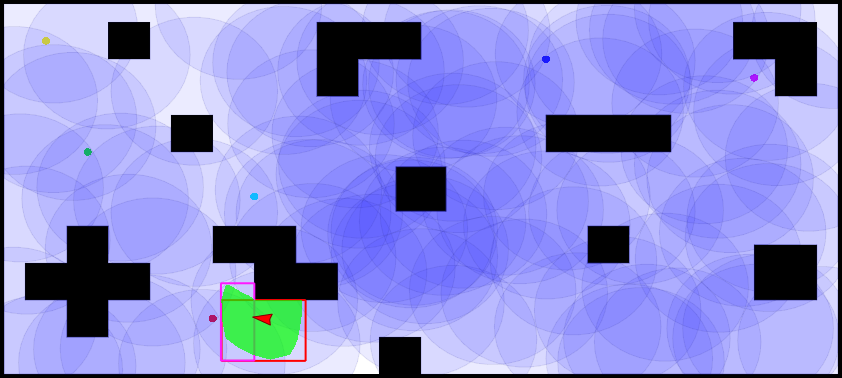
\includegraphics[width=.9\columnwidth]{figs/dbrect_clutter.png}
  \caption{A robot (red arrow) navigates itself in an environment with obstacles (black) and landmarks.
    The blue circles are the ranges in which the robot receive observations from the landmarks.
    The green region denotes the robot's true information state. 
    A union of two red boxes represents an over-approximation
    of the information state using double-rectangle.}
  \label{fig:nav-clutter}
\end{figure}

\subsection{Multi-Robot Formation}

As modern robotic research and technology arise, advances and new challenges
involve not only single robots but also large systems of robots. 
Needless to say, well-collaborated work often enhances the effectiveness, flexibility and
fault-tolerance of a single entity. 
A vivid example is shown in the movie ``Big Hero 6'', in which many small robots can configure and re-shape themselves to different formations to accomplish different tasks.
Hereby, research about multi-robot systems, on ground, or in aerial, or under water, attracts a growing number of attentions in recent years\cite{CaoFukKahMen95, DudJenMilWil96, BahSoySah03}. 
Groups of autonomous robots could be used for tasks ranging from exploring and mapping in an unknown environment to deploying large-scale mobile sensor network. 
However, in contrast to a single robot, the multi-robot systems normally raise more complicated problems, such as multi-sensor data fusion in the sensing procedure, or multi-robot collision
avoidance in the motion procedure and multi-robot coordination in the decision-making procedure.

We first describe a novel distributed algorithm that enables a group of mobile
robots to establish an arbitrary formation, including the repeated lattice
pattern, such as the geometric shapes of squares, hexagons, octagons, etc.
Figure~\ref{fig:octsq-init-final} shows an example in which $100$ robots formed 
a repeating octagon-square lattice pattern from a random initial distribution.
\begin{figure}
  \centering
  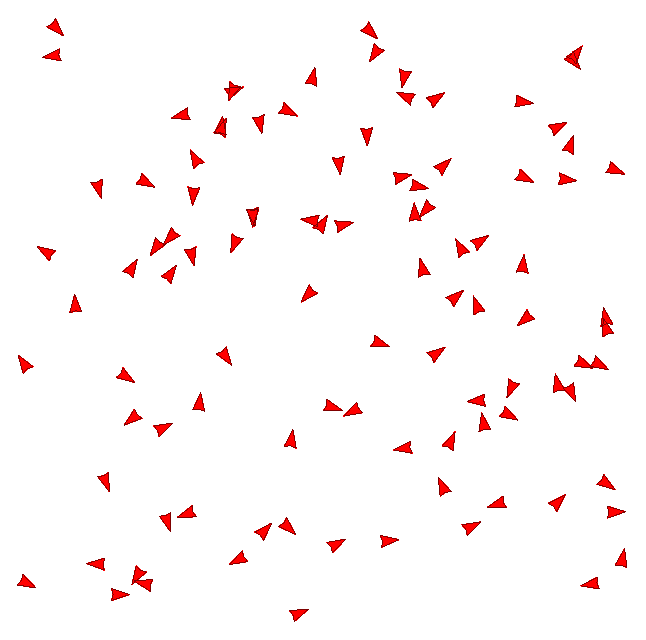
\includegraphics[width=.4\columnwidth]{figs/initial-formation}
  \bigskip
  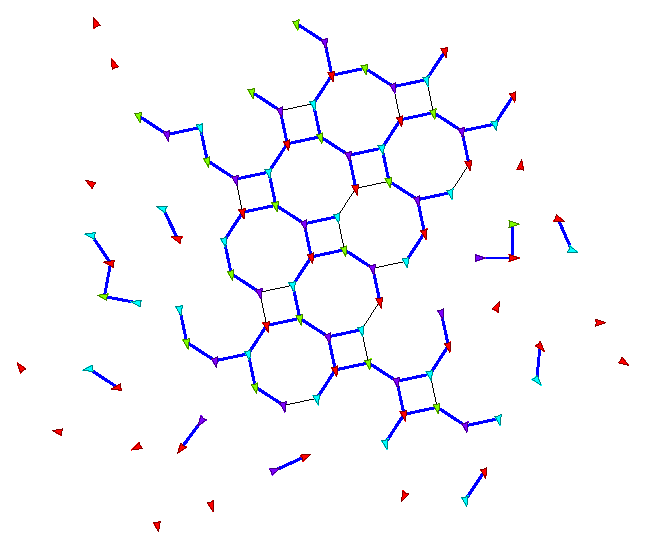
\includegraphics[width=.45\columnwidth]{figs/final-formation}
  \caption{[left] The initial poses of $100$ robots, randomly generated with a
  uniform distribution. [right] The final formation after executing our
  algorithm using the octagon-square lattice graph as an input.}
  \label{fig:octsq-init-final}
\end{figure}
We consider the multi-robot formation problem in a combination of the task
assignment problem~\cite{Kuh55, Mun57} and a graph matching
problem~\cite{Lov86}. Therefore, the major contributions of our work include (1)
a general graph representation of desired formation, called ``lattice graph'',
(2) a novel scheme called ``authority'' to organize the robots into a
globally rooted tree structure, which serves for the local task assignment, 
and (3) a series of experiments to verify the effectiveness of our algorithm.

However, the above-mentioned formation algorithm has two critical limitations.
\begin{enumerate}
\item There is no guarantee that the robots will eventually form the
  desired formation and terminate the algorithm. 
  Instead, the robots may oscillate under some conditions.
\item The motion strategy may cause some robots become
  disconnected with others (Figure~\ref{fig:octsq-init-final}), 
  thus, would bring side effects to the overall solution quality.
\end{enumerate}

To resolve these limitations, we have developed a new scheme by introducing a new communication protocol and a new motion strategy. 
In contrast to the prior algorithm which allocates multiple robots local destinations simultaneously,
the key idea of our new algorithm is relocating only one robot to a position to form the desired pattern sequentially.
Moreover, we have proved the correctness of our formation algorithm: (1) the
output of the algorithm correctly matches the goal lattice pattern, (2) the
algorithm has a time-bounded performance and improved final formation quality, 
compared with the results using the prior formation algorithm.

Chapter~\ref{chp:cga} describes the constrained geometric approximation method 
including: the review of the state-of-the-art,
the problem statement along with the fundamental knowledge related with the
information state, the detail of the algorithm, the experimental results, and conclusions.

In Chapter~\ref{chp:mrf}, we introduce the fundamental concepts of the multi-robot lattice formation problem we want to solve. 
% 
First we overview the related work. 
%
Then we address the problem by defining the robot model, the graph representation of the algorithm input, and the evaluation criteria for the algorithm output. 

Chapter~\ref{chp:mrf1} presents the framework of our primary stateless, task-assignment-based formation algorithm. 
%
We explain the definition of the robot authority and then describe the distributed task-assignment strategy in detail.
%
Also, we illustrate the experiments setup and conclude the method according to the simulation results.

Chapter~\ref{chp:mrf2} extends our discussion about the multi-robot lattice formation problem in Chapter~\ref{chp:mrf}, but focuses on a new decentralized algorithm. 
First we outline the limitations of the first algorithm, then describe the details of our new solutions.
Furthermore, we prove the algorithm correctness and analyze the time complexity of the new algorithm.
In the final part of Chapter~\ref{chp:mrf2}, we compare the experimental results of both algorithms, and evaluate the new method.

Chapter~\ref{chp:conc} gives a comprehensive summary of this dissertation and discusses about the future work.
    %% Calls Introduction.tex
%                           %% Honors theses are required to 
%                           %% have an Introduction.  For
%                           %% Honors theses, the file 
%                           %% Introduction.tex should begin
%                           %%
%                           %% \chapter*{Introduction}
%                           %% followed by the text of the 
%                           %% introduction.

\chapter{Constrained Geometric Approximation}
\label{chp:cga}

In this chapter, we focus on the planning problem for the robot subject to bounded
motion and sensing uncertainty.

The idea of representing and eliminating the uncertainty in a range space is inspired by O'Kane's
work~\cite{OKa11}. The author solved a decentralized tracking problem by letting
robots maintain proximity to a collection of unpredictably moving targets using
low-resolution sensors. Similarly, we over-approximate a robot's information state 
by constraining the geometric operations to produce sets within the range space. 
Our contributions stated in this chapter include new operations defined for the range space 
and the algorithm carrying out those operations. 

We organize the remaining of this chapter as following: in Section~\ref{sec:related-cga}, 
we review prior research related to our work. 
%
We define the problem formulation and describe the robot model as well as the
fundamental notations related to the information space in Section~\ref{sec:robot-mod} and Section~\ref{sec:ispace}. 
In Section~\ref{sec:rspace}, we define two operations
associated with the range space and discuss about the constrained geometric
approximation algorithm in detail. In Section~\ref{sec:simu-cga}, we provide groups of
experiments and collect the simulation results to evaluate the performance of our method
using different landmark-based navigation tasks. 
Based on the measurements of the computation time and the approximation quality of the algorithm
against three types of range spaces, we draw conclusions of our approach in the last section.

%\clearpage
\section{Related Work}
\label{sec:related-cga}
Most of prior work in robotics research community represented and reasoned about
the robot's uncertainty using probabilistic models. Especially for the
robot's navigation, simultaneous localization and mapping (SLAM), and searching problems, etc.,
the probabilistic approaches are well studied and widely used \cite{ThrBurFox98,
  ThrBurFox00, ThrBurFox05,JenKri01,SimKoe95,ThrBee+00,
  TomYut01,KamManMin96}. 
Thrun, Burgard, and Fox developed an algorithm for
landmark-based localization and mapping in the indoor environments where
the landmarks' locations and robot's positions are estimated by a likelihood
maximized under probabilistic constraints~\cite{ThrBurFox98}. In their work, the
probabilistic models were used to represent and reason about both of robot's
sensing and motion. 
Bayesian estimation algorithms were also used in Thrun's
work~\cite{Thr01} to estimate the robots' states from sensor measurements,
in order to conduct the concurrent mapping and localization tasks. 
Simmons and Koenig developed a navigation approach based on the partially observable Markov models
to track the location of the robot and maintains a probability distribution over all
possible locations with sensing and motion uncertainty~\cite{SimKoe95}.
Jensfelt and Kristensen solved a global localization problem using
probabilistic approach based on the topological world models, in which a Kalman
filter~\cite{Kal60} was applied to represent and track a number of pose
hypotheses of the robot~\cite{KuiByu91}. 

More recent work has used such probabilistic representations explicitly for
motion planning~\cite{KufLav00,PepKieWal09,BerAbbGol11,PreRoy09}. 
Kuffner and LaValle proposed a probabilistically complete randomized data structure called
rapidly-exploring random tree (RRT) for path planning~\cite{KufLav00}.  
Pepy, Kieffer, and Walter addressed the path planning problem by combining RRT and the set
representation of states with bounded uncertainty, they developed a ``Box-RRT'' path
planner and applied the method to nonholonomic vehicles. 
Berg, Abbeel and Goldberg presented a linear-quadratic Gaussian motion planning (LQG-MP) algorithm that
based on the linear-quadratic controller with Gaussian models of motion and
sensing noise~\cite{BerAbbGol11}. 
Prentice and Roy presented a planning algorithm for the linear Gaussian systems in belief (information) space to compute the reachable belief (information) state and find the path with minimum
expected cost, by reducing the computational cost of the extended Kalman filter
predictions~\cite{PreRoy09}.

The probabilistic approaches, including but not limited to above-mentioned work,
demonstrated considerable success in solving SLAM, navigation, and path planning problems. 
However, probabilistic methods are often computationally expensive. 
For example, Kavraki, Svestka, Latombe and Overmars presented an approach to construct the probabilistic roadmap in the high-dimensional collision-free configuration spaces~\cite{KavSve+96}. 
This technique may require the connections of thousands of configurations or states
to find a solution.
Another example is the usage of the Monte Carlo methods for localization problems:
the particle filters is often implemented with hundreds or thousands of particles~\cite{ThrFox+00}. 
Therefore, these approaches could be impractical for robots with limitations of computing power.

Moreover, another fact that limits the usage of probabilistic methods is that it
is difficult for the robot to decide how sufficiently many particles are
necessary to guarantee the convergence to the correct solution, based on a
realistic consideration of maintaining a relative small number of particles. 

Motivated by the idea of finding approach fitted to the robot applications 
with extreme limited computational capability, we developed a method
to maintain a set of the over-approximation of true information state, in
contrast to the particle filtering. 
Therefore, the robot can directly determine when the information it represents 
is not useful because of the insufficient detail of true I-state.

Another branch of robotics research, which has described itself as a ``minimalist''
approach, for example, following algorithms solved the problems in spite of limitations
in the robot's sensing capability~\cite{AkeMas98,Erd86, % manipulation
  KamRiv97, LumTiw94,BluRagSch97,LazLat92, %navigation
  TovGuiLav04, AcaCho01b,ChoBur00}. %mapping}.
Akella and Mason introduced a classification of polygonal objects subject to
linear pushing actions. They described a complete pose planner to
construct a sequence of pushing actions to move a polygonal object from any
initial pose to any final pose regardless of the feedback sensing~\cite{AkeMas98}. 
%
Kamon and Rivlin presented a planning algorithm using the range data, 
this approach ensures to navigate the robot to reach the target in an unknown environment or to report the target is unreachable~\cite{KamRiv97}. 
%
Lazanas and Latombe described a complete polynomial algorithm to solve a navigation
problem in spite of uncertainty. 
%
Given landmarks scattered across the environment, the planner computes a plan with bounded uncertainty by
backtracking the omnidirectional back-projections of the goal, until one fully
contains the set of possible initial positions of the robot~\cite{LazLat92}.
%
Tovar, Guilamo and LaValle presented a data structure of the ``Gap Navigation Tree''
(GNT) to solve different visibility-based tasks with minimal sensing requirements in unknown planar environments, 
whose boundaries were piecewise smooth closed curves, with finite number of non-smooth points~\cite{TovGuiLav04}. 
The GNT structure reflects the path information in the information space, 
it is constructed from the online sensor measurements and updated during the robot's moving. 
%
Tovar, LaValle and Murrieta also showed that robots can complete the tasks such as navigation~\cite{TovLavMur03b}, pursuit-evasion~\cite{TovLav06}, etc., using the GNT approach.
%
Acar, Choset and Atkar conducted work on the sensor-based coverage path planning method to
determine a path that passes a detector, whose range extended beyond the robot's
periphery, over all points in an unknown environment~\cite{AcaCho01b}. 
%
They combined approaches of the sensor-based coverage algorithm~\cite{AcaCho01a,AcaCho00, ChoAcaRizLun00} and the motion planning algorithm used to navigate the robot along the generalized Voronoi diagram~\cite{ChoKonRiz97, ChoBur00} to completely cover an obstacle-free space with an infinite-range
detector. 
%
Tokekar and Isler worked on the problem of placing bearing sensors with bounded uncertainty for robot localization~\cite{TokIsl13}. 
They showed that, given a fixed number of nearby sensors, the robot can localize itself in an unknown environment without losing much estimation quality.

However, these methods generally consider the assumptions of the robot's sensing limitations, 
but not in computation. 
%
In contrast to the complicated procedure of computing the true I-state~\cite{TovLav08, YuLav10}, 
our work contributed to demonstrate that such precise I-states are not always necessary for a robot to complete its task.
Additionally, it is much more efficient to compute reasonable constrained approximations~\cite{SonOka12}.

%\clearpage
\section{Robot Model}
\label{sec:robot-mod}
We consider the point robot in our problem and assume that the robot can not reason about
its state from the observations directly. 
%
Instead, the robot maintains a set of all possible states from its observations. 
%
The robot model contains following concepts in detail.
\begin{enumerate}
\item \emph{State space} $X = \Real^2$: a discrete state space $X$ is
  partitioned into obstacle space $X\sub{obst}$ and obstacle-free space
  $X\sub{free}$. The state of the robot at stage $k \in \Natural$ is written as
  $x_k$.
\item \emph{Action space} $U$: the robot chooses one action $u_k \in U$ which is
  addictive to the state at each stage.
\item \emph{State transition function} $F : X \times U \to \pow(X)$: a
  set-valued transition function is used to describe how does the robot's state $x_k$
  change along with an action $u_k$, with $x_{k+1} \in F(x_k, u_k)$. The
  $\pow(X)$ denotes the powerset of $X$. We consider an addictive noise
  $\theta_k$ to robot's action $u_k$, and we also assume the bounded set of
  uncertainty for a certain action, denote as $\Theta(u_k)$, such that
  \begin{equation}
    \label{eq:state-trans}
    F(x_k, u_k) = \left\{
      x_k + u_k + \theta_k
      \mid
      \theta_k \in \Theta(u_k)
    \right\} \cap X\free.
  \end{equation}
  We assume the bounded noise on both the direction and magnitude of the robot's
  action. 
  The angular noise is bounded by a fixed angle $\delta\sub{ang}$, and
  the translation noise is bounded by $\delta\sub{trans}||u||$. 
  Thus, the
  transition noise set $\Theta(u_k)$ is a slice of an annulus (Figure~\ref{fig:noiseModel}).
  \begin{figure}
    \centering
    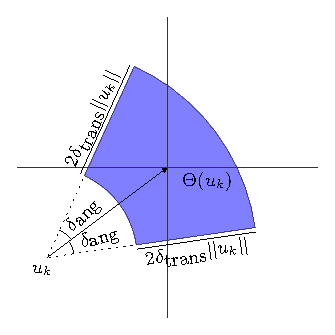
\includegraphics[scale=1.2]{figs/noisemodel}
    \caption{The noise model $\Theta(u_k)$ involves bounded angular error
      $\delta\sub{ang}$ and bounded translational error
      $\delta\sub{trans}||u||$.}
    \label{fig:noiseModel}
  \end{figure}	

\item \emph{Observation space} $Y$: an observation at stage $k$ is the sensor
  information collected by the robot, denoted as $y_k \in Y$.
\item \emph{Observation function} $h : X \to \pow(Y) $: we use a set-valued
  function to model the robot's observations, the set-valued nature of this function reflects
  that the sensing in our problem formulation can not be fully predicted. Also
  define a function
  \begin{equation}
    \label{eq:preimage}
    H(y_k) = \left\{ x_k \in X \mid y_k \in h(x_k), y_k \in Y \right\},
  \end{equation}
  in order to retrieve the set of states from which a given observation might be obtained.
\item \emph{Initial condition} $\eta_0$: initially we assume that we know a set
  $\eta_0$ containing all possible starting states of the robot, namely,
  $\eta_0$ represents a set $X_1\subseteq X$. 
\end{enumerate}

%\clearpage
\section{Information Space}
\label{sec:ispace}
The problem we address here is in a scenario in which the robot is able to complete
tasks without knowing the exact states. 
%
Therefore, the planning algorithm can be considered in terms of the information space respective.  
%
The ultimate objective of our approach is to form a plan $\pi$ which the robot can execute using the
information available in the information space.
%
Generally, an information space is essentially a special state space which involves the history of action and sensor observation. 
%
Here we follow the convention from LaValle's book~\cite{Lav06}. 
%
Assuming at every stage robot collects sensor observations and makes an action. 
The sensor history at stage $k$ is
\begin{equation}
  \label{eq:sensor-hist}
  \tilde{y}_k = (y_1, y_2, \ldots, y_k).
\end{equation}
The action history at stage $k$ contains every action from when the first action
was applied to the time when the latest action $u_{k-1}$ was applied. 
Thus, we have
\begin{equation}
  \label{eq:action-hist}
  \tilde{u}_{k-1} = (u_1, u_2, \ldots, u_{k-1}).
\end{equation}

\begin{defn} 
  A state $x_k \in X$ is \emph{consistent with} a sensor-action history
  $(\tilde{y}_k, \tilde{u}_{k-1})$ if there exists some state sequence
  $x_1,\ldots,x_{k+1} \in X$ such that $x_1 \in \eta_0$, and $x_{i+1} \in F(x_i,
  u_i)$ for each $i=1,\ldots,k$, and $y_i \in h(x_i)$ for each $i=1,\ldots,k+1$.
\end{defn}


\begin{defn}
  \label{def:istate} 
  The \emph{information state} (I-state) $\eta_k$ at stage $k$ is the set of all
  states consistent with the robot's sensor-action history.
\end{defn}


We can compute the history
I-state by combining the sensor-action history with the initial condition.
%
Denote the history I-state at stage $k$ using $\eta_k$, we have
\begin{equation}
  \label{eq:hist-istate}
  \eta_{k+1} = (\eta_0,\tilde{u}_{k},\tilde{y}_{k}).
\end{equation}
%
We noticed that the history I-state at stage $k+1$ contains all the information from
I-state at $k$ plus the latest observation $y_{k+1}$ and most recently applied
action $u_{k}$, we can write $\eta_{k+1}$ as
\begin{equation}
  \label{eq:hist-istate2}
  \eta_{k+1} = (\eta_{k}, {u}_{k}, y_{k+1}).
\end{equation}

\begin{defn}
  \label{def:ispace} 
  The \emph{information space} (I-space) $\Ispace$ is the
  powerset of $X$, which contains all possible I-states.
\end{defn}


Since the exact state $x_k$ is known to be contained in the I-state $\eta_k$, we
let $X(\eta_k) \subseteq X$ be the minimal subset in the state space consisted
with $\eta_k$. 
%
Recall Equation~\ref{eq:preimage}, we could infer the possible states from sensor observation $y_k$, $X_k(\eta_k) \subseteq H(y_k)$. 
%
Thus, starting from the initial condition, the robot updates its knowledge of 
possible states in terms of the history of its actions and observations. 


The base case for stage $1$ is formulated as:
\begin{equation}
  \label{eq:initial-istate}
  X_1(\eta_1) = X_1(\eta_0, y_1) \cap H(y_1).
\end{equation}
%
Assume that $X_k(\eta_k) \subseteq X$, $X_{k+1}(\eta_{k+1})$ can be inductively
computed. 
Recall Equation~\ref{eq:hist-istate2}, we have $\eta_{k+1} =
(\eta_{k}, {u}_{k}, y_{k})$, such that
\begin{equation}
  X_{k+1}(\eta_{k+1}) = X_{k+1}(\eta_{k}, {u}_{k}, y_{k}).
\end{equation}
%
Then we apply two set operations to compute the state subset
$X_{k+1}(\eta_{k+1})$: 
\begin{enumerate}
\item apply set union with the output of state transition function (Equation~\ref{eq:state-trans}) on every possible states contained in $X(\eta_k)$, we yield:
\begin{equation}
  X_{k+1}(\eta_{k}, u_k) =  \bigcup_{x_k \in \eta_k} F(x_k, u_k);
\end{equation}
\item apply set intersection on the observation preimage at stage $k$ with the
state subset from the first step:
\begin{equation}
  \eta_{k+1} = X_{k+1}(\eta_{k}, u_k) \cap H(y_{k}).
\end{equation}
\end{enumerate}
%
Hence, $\eta_{k+1}$ can be iteratively computed from starting condition
(Equation~\ref{eq:initial-istate}) using Equation~\ref{eq:istate-trans}:
\begin{equation}
  \label{eq:istate-trans}
  \eta_{k+1} =
  \left[ \bigcup_{x_k \in \eta_k} F(x_k, u_k) \right].
  \cap H(y_{k}).
\end{equation}


Use the computed I-state, the robot can make decision on its action in order to
complete the task, so that the plan $\pi: \Ispace \to U$, $u_k = \pi(\eta_k)$.

%\clearpage
\section{Range Space}
\label{sec:rspace}
The updates of the information state is computationally expensive since each
I-state contains many states and sensor-action history. 
%
To simplify the representation of the I-state $\eta_k$, our approach maintains only an
over-approximation of the $\eta_k$, denote as $A_k$, so that
\begin{equation}
  \eta_k \subseteq A_k.
\end{equation}
%
The key idea of our approximation approach is to select a range space $\Rspace
\subseteq \Ispace$ within the I-space, and constrain the approximated I-space to
remain a member of this range space, so that $A_k \in \Rspace$.
\begin{defn}
  \label{def:rspace}
  A range space $\Rspace \subseteq \Ispace$ is a set of I-states, equipped with
  two functions:
  \begin{enumerate}
  \item an \emph{approximate action update function} $T: \Rspace \times U \to
    \Rspace$, such that if $\eta_k \subseteq A_k$, then
    \begin{equation}
      \label{eq:T}
      \bigcup_{x_k \in \eta_k} F(x_k, u_k) \subseteq T(A_k, u_k);
    \end{equation}
  \item an \emph{approximate observation update function} $O: \Rspace \times
    Y \to \Rspace$, such that if $\eta_k \subseteq A_k$, then
    \begin{equation}
      \label{eq:O}
      \eta_k \cap H(y_k) \subseteq O(A_k, u_k).
    \end{equation}
  \end{enumerate}
\end{defn}
%
Similar to the information space, the approximation set $A_{k+1}$ containing the
I-state $\eta_k$ in the range space can be iteratively computed from an initial
state $A_0 = \eta_0$:
\begin{equation}
  A_{k+1} = O(T(A_k, u_k), y_{k}).
\end{equation}
%
We have used different types of geometric sets to approximate the I-state. 
%
The intuition is that we can use simple data structures to save all possible states
$x_k$ contained in the exact I-states such that $x_k \in A_k$.

\subsection{Disk Range Space}
\label{subsec:disk}
First we consider a circular approximation of the true I-state. 
%
In view of the computational efficiency, a circle or planar disk can be quickly parameterized
by a center point and a radius. 
%
Denote the set of all disks in $\Real^2$ using $\Rdisk$. 
Recall in a 2D plane, an information state can be represented using a compact set, 
thus, for any compact set $S \subset \Real^2$, let $\sed(S)$ denote the smallest disk enclosing $S$.
%
Then we define
\begin{flalign}
  \label{eq:tdisk} 
  T\disk(A_k, u_k) = A_k \oplus \{ u_k \}
  \oplus \sed(\Theta(u_k)).
\end{flalign}
%
In Section~\ref{sec:robot-mod}, we have mentioned that the action and
noise models in this problem are under addictive operation.
%
Hence, for two sets of pointer vectors, we apply the Minkowski sum operation~\cite{DebVanOveSch97}, denoted
using operator $\oplus$. 
%
Computing Minkowski sums of disks consists of the addition of their centers and radius, therefore, it takes constant time to compute $T\disk$.  
%
When the observation preimages are quarter-planes or circles, 
computing the $O\disk$ also takes constant time~\cite{OKa08b, OKaXu12}.
%  
Because both $A_k$ and $\sed(\Theta(u_k))$ are disks, the result is still in $\Rdisk$.  
%
Similarly, we define
\begin{equation} 
  O\disk(A_k, y_{k}) = \sed(H(y_{k}) \cap A_k).
\end{equation} 
It is trivial to show that $\Rdisk$ is a range space under the
operations of the action update and the observation update by definition.

\subsection{Rectangle Range Space}
\label{subsec:rect}
Denote an axis-aligned rectangle approximation set as $\Rrect \subset \Real^2$, 
each set can be simply represented by its lower left corner $a$ and
its upper right corner $b$. 
%
Similar to the $\sed$ operation in the $\Rdisk$, we define an operation to find the minimum axis-aligned rectangle given a compact set $S \subset \Real^2$.
We name the operation $\aabb(S)$, short for ``axis-aligned bounding box.''
%
Then, we can define
\begin{flalign}
  \label{eq:trect} 
  T\rect(A_k, u_k) = 
  \aabb(X\free \cap [A_k \oplus \{u_k\} \oplus \aabb(\Theta(u_k))]).
\end{flalign} 
%
Also we define the approximate observation update function:
\begin{equation}
  \label{eq:orect} 
  O\rect(A_k, y_{k}) = \aabb(H(y_{k}) \cap A_k).
\end{equation} 
%
By definition, we can show that $\Rrect$ is a range space under $T\rect$ and $O\rect$.

Figure~\ref{fig:rect-update12} and Figure~\ref{fig:rect-update34} illustrate the steps to
compute the approximation set $A_{k+1}$ using the approximate transition function $T\rect$ in the rectangle range space, as described in Equation~\ref{eq:trect}.

\begin{enumerate}
\item Step 1: find the minimal axis-aligned bounding box for the bounded noise set
  $\Theta(u_k)$ of action $u_k$, $\aabb(\Theta(u_k))$. 
  Since the set $\Theta(u_k)$ is represented as a list of vertices on its boundary, this
  operation takes linear time to find the extremal coordinates in each direction
  from the vertex list.

\item Step 2: compute the Minkowski sum $A_k \oplus \{ u_k \} \oplus \aabb(\Theta(u_k))$, 
  using the result of Step 1. 
  This step takes constant time because each of the three operands is either a single point or a rectangle
  represented by its lower left and upper right corners, the results can be
  computed by adding the coordinates of the respective corners together.
	
\item Step 3: intersect the free state space $X\free$ with the result of Step
  3, using the general polygon clipping algorithm~\cite{Vat92}. 
  This step yields a polygonal region that contains $\eta_k$.

\item Step 4: apply the same algorithm in Step 1 to find the axis-aligned
  bounding box of the result of Step 3. 
  Hence, we assure that the computed approximation set $A_{k+1} \in \Rrect$.
\end{enumerate}
\begin{figure}
\centering
  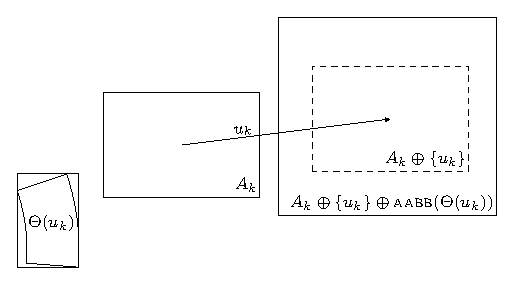
\includegraphics[scale=1.2]{figs/rect-update2}  
  \caption{Steps 1 and 2 of proceeding approximate observation update function}
  \label{fig:rect-update12}
\end{figure}

\begin{figure}
  \centering
  \begin{minipage}[b]{0.45\linewidth}
    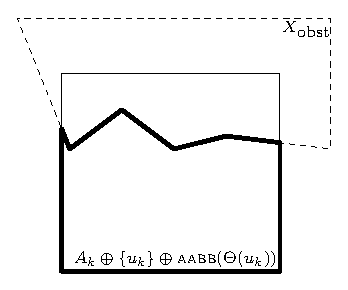
\includegraphics[scale=1.25]{figs/rect-update3}% \\  \hfill
  \end{minipage}
  \bigskip
  \begin{minipage}[b]{0.45\linewidth}
    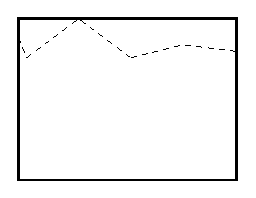
\includegraphics[scale=1.25]{figs/rect-update4}
  \end{minipage}
  \caption{Steps 3 and 4 of proceeding the approximate action update function}
  \label{fig:rect-update34}
\end{figure}

According to Equation~\ref{eq:orect}, the approximation set can be updated with
the observation preimage. 
%
We let the observation preimage be a disk in $\Real^2$, the intuition is to accelerate the computation by modeling the preimage using a specific known shape, such as disk or other geometric shapes. 
%
In our experiments, every $H(y_k)$ is modeled using a planar disk.  
In that case, we can compute $O\rect(A_k, y_k)$ in constant time using following
steps (Figure~\ref{fig:orect}): 
\begin{enumerate}
\item Step 1: compute the set of points at which the boundary of the disk
  $H(y_{k})$ intersects the boundary of the rectangle $A_k$. 
  There are at most $8$ such points.
  
\item Step 2: for each of four axis-aligned extremal points of the disk
  $H(y_{k}),$ that is, its topmost, bottommost, leftmost, and rightmost
  points, check if it is a subset in $A_k$.

\item Step 3: find the minimum axis-aligned rectangle that contains the
  8 or fewer points found in Steps~1 and 2.
\end{enumerate}

\begin{figure} 
  \centering
  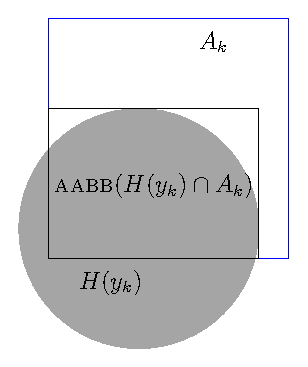
\includegraphics[scale=1]{figs/circlerect}
  \caption{Computing $O\rect(A_k, y_{k})$ to find the rectangle approximated I-state, 
    given an observation $y_{k}$.}
  \label{fig:orect}
\end{figure}

\subsection{Double-Rectangle Range Space}
\label{subsec:dblrect}
Using the geometric shapes, such as disk, or rectangle, to
approximate the I-state limits to provide good approximations
when the exact I-state $\eta_k$ is not a convex set. 
That is, the over-approximation set could be far from close to the true I-state in this case.

To overcome this limitation, our work contributes to a novel range space,
\emph{double-rectangle}, which is essentially a union of two rectangular
regions, for both convex and non-convex I-states over-approximation:
\begin{equation}
  \Rdrect = \{ R_1 \cup R_2 \mid R_1, R_2 \in \Rrect \}.
\end{equation}

To make the new range space useful, we have to define a function that enforces the $\Rdrect$ 
to be a range space under operations of the action transition (Equation~\ref{eq:T}) 
and the observation update (Equation~\ref{eq:O}).

We introduce an algorithm called $\drap$, short for the term ``double rectangle
around polygon'', which accepts a polygonal region in $\Real^2$ as input, and
outputs a small double-rectangle containing that polygon.  
%
The intuition of this algorithm is to maintain the size of the resulting double-rectangle as small
as possible, but not necessarily minimum in view of the computation efficiency.

\begin{figure} 
  \centering
  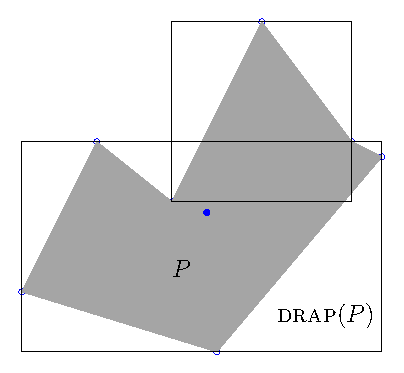
\includegraphics[scale=1]{figs/doublerect}
  \caption{A double-rectangle around the given a non-convex input polygon $P$}
  \label{fig:drap}
  %}
\end{figure}

Figure~\ref{fig:drap} shows an example of the executing the Algorithm~\ref{alg:drap}. 
%
The $\drap$ algorithm uses a bottom-up manner to find the double rectangle. 
%
Starting with two degenerate rectangles, each one is a single point at either a vertex of the polygon or at its centroid, as ``seeds''.
%
Then an iterative process considers each edge of the polygon in turn, and
expands one of the two rectangles to contain that edge.  
%
In each iteration, we choose between the two possible expansions by greedily preferring the rectangle
to expand that results in the smallest total area.  
%
Finally, to ensure that the result does not contain any unnecessary over-approximation, 
we repeat this process over all pairs of potential seed points, and retain only the smallest
overall double rectangle, as measured by its area. 
%
For a polygon with $n$ vertices, this algorithm takes $O(n^3)$ time.
% 
The outer loop runs $O(n^2)$ times since there are $C_n^2$ pairs of vertices, in
which $C_n^2$ is a binomial coefficient. The inner loop runs $O(n)$ times.

With the Algorithm~\ref{alg:drap}, we show that $\Rdrect$ is in a range space by definition.
%
For a double-rectangle I-state approximation $A_k = R_1 \cup R_2$, we have
\begin{flalign}
  \label{eq:dblrect-T}
  T\drect(A_k, u_k) = \drap(X\free \cap [A_k \oplus \{ u_k \} \oplus
  \drap(\Theta(u_k))]), \\
  O\drect(A_k, y_{k}) =  \aabb(H(y_{k}) \cap R_1)
  \cup \aabb(H(y_{k}) \cap R_2).
\end{flalign}

\begin{algorithm}
    \SetKwInOut{Input}{input}
    \SetKwInOut{Output}{output}
    \Input{A polygon $P$}
    \Output{A double-rectangle over-approximating $P$}
    $V \leftarrow $ a set containing the vertices of $P$ and its centroid\;
    $C \leftarrow $ a set containing double-rectangle approximations\;
    \ForEach {vertex pair $p,q \in V, p \neq q$}{
        $R_1 \leftarrow \{ p \}$; $R_2 \leftarrow \{ q \}$\;
	    \ForEach {edge $e \in P$}{
		    $R_1' \leftarrow$ $\aabb(R_1 \cup e)$\;
		    $R_2' \leftarrow$ $\aabb(R_2 \cup e)$\;
		    \eIf{$\area(R_1' \cup R_2) < \area(R_1 \cup R_2')$}{
		        $R_1 \leftarrow R_1'$\;
		    }{
		        $R_2 \leftarrow R_2'$\;
		    }
	    }
	    insert $R_1 \cup R_2$ into $C$\;
	}
    \Return
    $\operatornamewithlimits{argmin}_{(R_1 \cup R_2) \in C}(\area(R_1 \cup R_2))$\;
    \caption{Compute a double-rectangle approximation of a polygon}
    \label{alg:drap}
\end{algorithm}

%\clearpage
\section{Performance Evaluation}
\label{sec:simu-cga}
To evaluate the quality of the approximation throughout the robot's execution,
we can compare the area of the approximated I-state to the area of the
I-state itself:
\begin{equation}
  \label{eq:error}
  Q_k = \frac{1}{k} \sum_{i=1}^k \frac{\area(\eta_i)}{\area(A_i)}.
\end{equation}
The higher value of $Q$ demonstrates the better approximation quality, up to
a maximum value of $1$. 


\subsection{Navigation Task}
\label{subsec:nav}
One application of our method is that the robot can form a plan without
requiring to know its exact state in a landmark-based navigation task.  
%
In a known environment with or without obstacles, we placed landmarks in the
locations of $l_1,\ldots,l_m$ which can be detected by the robot. 
%
Each landmark has an detection range $\range_i, i \in [1, \ldots, m]$, therefore, the observation
preimage is a disk with center point at $l_i$ and radius $\range_i$. 
%
Moreover, to navigate the robot, we place a sequence of waypoints $w_1,\ldots,w_n$
such that each waypoint is visible and reachable 
by the robot from both its predecessor and its successor.

In order to complete the navigation task, the robot needs to form a plan of
sequentially visiting each of the waypoints, by utilizing the imperfect sensed
information and its noise movements. 
%
We consider a robot has successfully completed a task if and only if the robot finished visiting the waypoints in finite time. 
%
Otherwise, we consider the failure of a task if the robot collides with
an obstacle or it takes too long time to reach the final waypoint.

We denote the next waypoint by $w$ and select an action that moves toward $w$
from the centroid of $A_k$ in terms of plan $\pi(A_k)$:
\begin{equation}
  \label{eq:vhat}
  \pi(A_k) = \dfrac{w - \operatorname{centroid}(A_k)}{\|w- \operatorname{centroid}(A_k)\|} v\sub{max}.
\end{equation}

\subsection{Experimental Results}
\label{subsec:exp}
To verify the effectiveness and efficiency of CGA for the navigation task, we
conducted experiments using three distinct environments
(Figure~\ref{fig:env}), and three distinct range spaces: $\Rspace_{disk}$,
$\Rspace_{rect}$, and $\Rspace_{dblrect}$.  
%
We implemented the experiments using C++, and performed all the simulations on a GNU/Linux PC with Intel Core i7 CPU, 2.8GHz and 8GB memory.
We present experiments that measured these approximation ratios, 
along with the robot's success rate in completing the navigation task using each of these range spaces.
\begin{figure}
  \centering
  \begin{minipage}[b]{0.45\textwidth}
    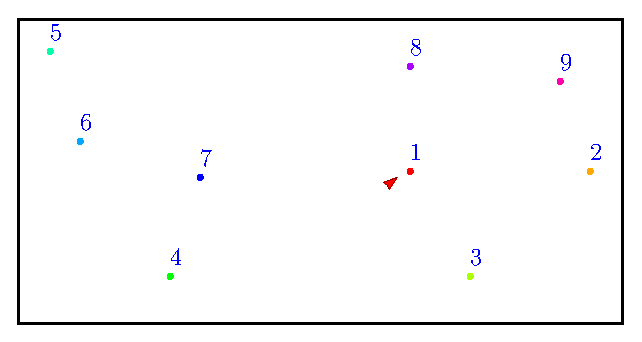
\includegraphics[scale=0.65]{figs/blank}  \\ 
    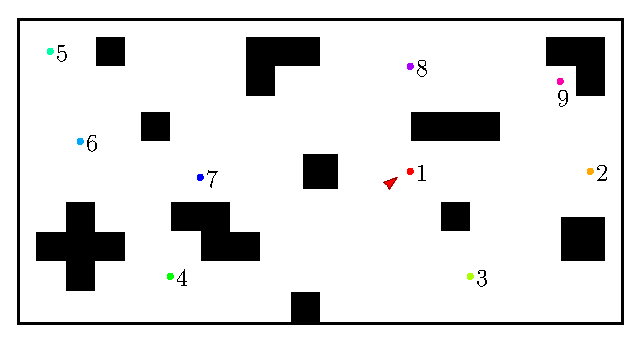
\includegraphics[scale=0.65]{figs/clutter}  
  \end{minipage}
  \begin{minipage}[b]{0.45\textwidth}
    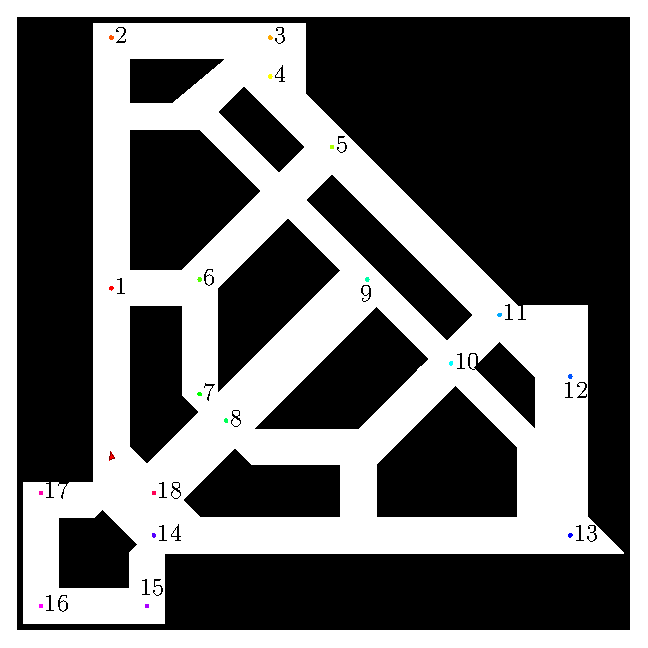
\includegraphics[scale=0.65]{figs/office}    
  \end{minipage}
  \caption{Three environments with landmarks: [top left] Obstacle-free. [bottom
    left] Obstacle-clutter. [right] Office-like.}
  \label{fig:env}
\end{figure}

\subsubsection{Task Completion Using CGA}
In each environment, we performed two series of experiments. 
%
First, we varied the number of landmarks $N$ between $5$ and $250$ in increments of $5$ and calculated the
robot's success rate.  
%
For each $N$, we repeated the experiment $15$ times with different landmark distributions generated from distinct random seeds. 
%
The success rate is the number of times that task completes successfully divided by
the total number of trials.  
%
Figures~\ref{fig:sucRate1}, \ref{fig:sucRate2}, and \ref{fig:sucRate3} show the average success rate for three environments, respectively. 
%
We conclude that using the approximated I-states can achieve similar performance as using the true I-state, 
especially when using $\Rrect$ and $\Rdrect$.

\begin{figure}
  \begin{center}
    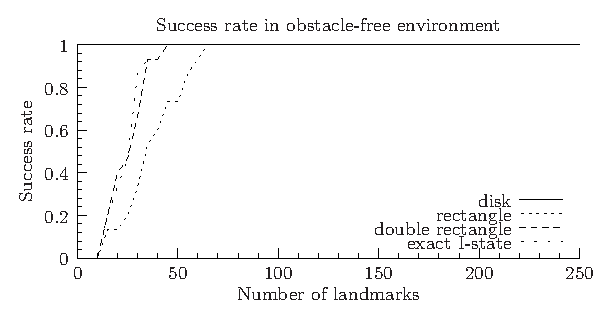
\includegraphics[width=0.95\textwidth]{figs/exp_num_blank}
  \end{center}
  \caption{The statistics of the success rate versus 
    the number of landmarks in the obstacle-free environment.}
  \label{fig:sucRate1}
\end{figure}
\begin{figure}
  \begin{center}
    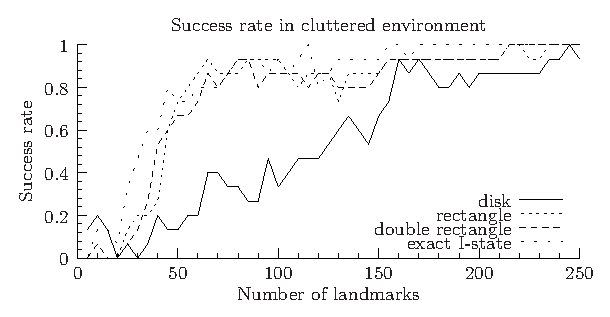
\includegraphics[width=0.95\textwidth]{figs/exp_num_clutter}
  \end{center}
  \caption{The statistics of the success rate versus 
    the number of landmarks in the obstacle-cluttered environment.}
  \label{fig:sucRate2}
\end{figure}
\begin{figure}
  \begin{center}
    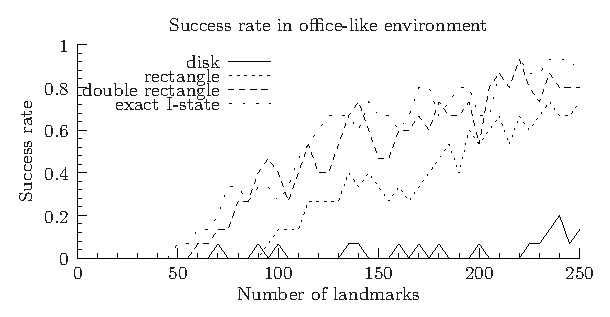
\includegraphics[width=0.95\textwidth]{figs/exp_num_cse}
  \end{center}
  \caption{The statistics of the success rate versus 
    the number of landmarks in the office-like environment.}
  \label{fig:sucRate3}
\end{figure}

Using $\Rdisk$ in the environments with obstacles yields the lowest success rate comparing to other range spaces. 
%
We conclude the reason as that $T\disk$ does not take the obstacles into account
(Equation~\ref{eq:tdisk}). 
%
We omit this step from $T\disk$ because computing $\sed$ for complex obstacle shapes is computationally expensive. 
%
The success rates of using three range spaces in the office-like environment
(Figure~\ref{fig:sucRate3}) are lower than the results in other
environments. 
%
The reason that directly impacts the performance is that there are more obstacles 
and narrow corridors in this environment. 
%
Meanwhile, after comparing the success rates of using different range spaces in the same environment, 
we conclude that using the double-rectangle approximated I-states provides better
performance over using the other types of range spaces.


Moreover, we conducted experiments to evaluate the impact of the selection of axes. 
%
Consider both $\Rrect$ and $\Rdrect$ range spaces, they are constructed based on only
axis-aligned rectangles. 
Therefore, we have comprehensively evaluated the performance of the CGA method by performing these experiments below.
%
We rotated each environment for a degree between $0$ and $2\pi$ radians, in increments of $\pi/12$, 
and executed $10$ trials with $250$ landmarks in each environment.
%
Figures~\ref{fig:sucRate4} and \ref{fig:sucRate5} show the success rates of
using three range spaces in two environments with obstacles. 
%
We omit the results for the obstacle-free environment here since the robot always accomplished the
navigation task in each trial. 
%
Above all, the results have demonstrated that there is no substantial degradation 
of CGA's performance as a function of environment rotation.


\begin{figure}
  \begin{center}
    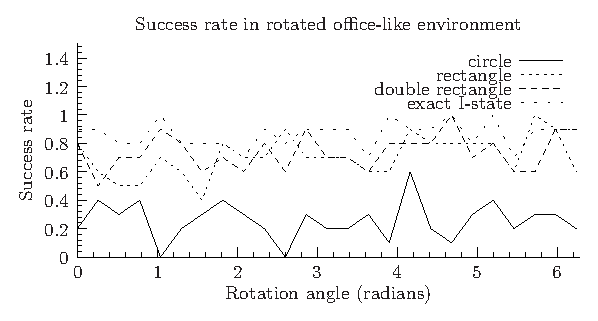
\includegraphics[width=0.95\textwidth]{figs/exp_rot_cse}
  \end{center}
  \caption{The statistics of the success rate versus 
    the number of landmarks in the rotated office-like environment.}
  \label{fig:sucRate4}
\end{figure}

\begin{figure}
  \begin{center}
    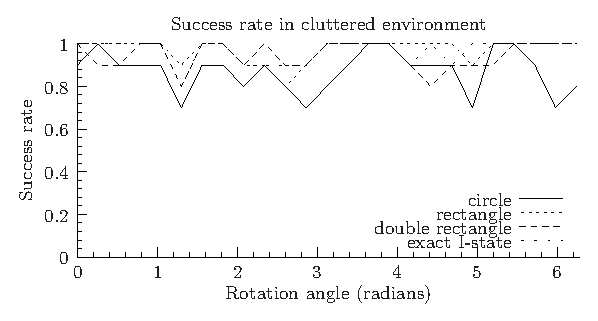
\includegraphics[width=0.95\textwidth]{figs/exp_rot_clutter}
  \end{center}
  \caption{The statistics of the success rate versus 
    the number of landmarks in the rotated obstacle-clutter environment.}
  \label{fig:sucRate5}
\end{figure}

\subsubsection{Computation Time and Approximation Quality}

We also conducted experiments to compare the computation time of our approximated
I-states with the corresponding computation time of the exact I-states.  
%
We used $N=300$ landmarks and conducted $10$ trials for each combination of the range space
and the environment.  
%
At the same time, we compute the approximation ratio $Q$ as defined in Equation~\ref{eq:error}.  
%
From the results shown in Table~\ref{tab:exp-data}, 
we conclude that there is a trade-off between the computation time and the approximation quality of using different range spaces. 
%
Moreover, the results demonstrate that using the double-rectangle range space could produce the highest approximation quality.

\begin{table}
  \small\centering
  \caption{Experimental results: computation time and approximation
      ratio for range spaces and I-space in three testing environments.}
    \begin{tabular}{ccccccc} 
    \toprule 
    Range  & \multicolumn{2}{c}{Obstacle-free} & \multicolumn{2}{c}{Clutter} & \multicolumn{2}{c}{Office-like}\\
    Space & Time(s) &Approx.Ratio& Time(s) &Approx.Ratio& Time(s) &Approx.Ratio \\
    \midrule
    $\Rspace_{disk}$ & 0.163 & 0.155 & 0.162 & 0.155  & 0.292 & 0.220 \\ 
    \midrule
    $\Rspace_{rect}$ & 0.396 & 0.642  & 0.441 & 0.632 & 0.415 & 0.661 \\
    \midrule
    $\Rspace_{dblrect}$ & 1.021 & 0.684 & 1.122 & 0.691 & 1.491 & 0.720 \\
    \midrule
    $\Ispace$ & 10.074 & 1.000 & 10.218 & 1.000 & 26.895 & 1.000 \\
    \bottomrule     
    \end{tabular}
    \label{tab:exp-data}
\end{table}


The results of these experiments have verified the effectiveness of our over-approximating approach.
%
Specifically, the innovation of the range space as the union of
two rectangles improves the approximation accuracy. 
%
We conclude that our method of representing a robot's uncertainty and reasoning about its state is useful 
for robot to complete specific tasks, such as navigation task based on the landmarks, even subject to a low approximation ratio.

However, it remains as future work to consider additional range spaces.  
%
Particularly, we can extend this approach to a general method to approximate the exact I-state using $k$-fold unions of rectangles, 
without any substantial changes to the algorithm.  

We can expect the trade-offs between accuracy and efficiency that are exposed by using
larger numbers of rectangles in the approximated I-state.  

Furthermore, the range spaces that allow more general polygonal shapes are worthy to be considered. 
The challenge is how to maintain efficiency by limiting their number of vertices, 
and by applying appropriate expansion operations to enforce this limit.




\chapter{Multi-Robot Lattice Formation Problem}
\label{chp:mrf}

In this chapter, we address a multi-robot lattice formation problem.
%
Consider a set of a large number of autonomous robots, in which each
robot can only use local information, 
we focus on a problem that the robots want to form an arbitrary lattice patterns autonomously.


The remaining sections of this chapter are organized as follows. 
%
Section~\ref{sec:related-mrf} gives a summary of related work on the multi-robot formation problems.
%
Specifically, we review the work focusing on solving the problems in a distributed manner. 
%
Section~\ref{sec:robot-model} illustrates the robot model we have used in this multi-robot lattice formation problem.
%
Section~\ref{sec:latt-graph} introduces the graph concepts we have used to represent the output lattice pattern in our problem formulation, and to analyze the robots' communication activities. 
%
Section~\ref{sec:mrf-eval} defines two criteria we have used to evaluate our formation algorithms.
%
All of the robot model, the lattice graph, and the evaluation criteria are common concepts used by two types of formation algorithms in Chapter~\ref{chp:mrf1} and Chapter~\ref{chp:mrf2}.

%\clearpage
\section{Related Work}
\label{sec:related-mrf}

A distributed solution is powerful and efficient to many applications of the multi-robot systems,
such as deploying multiple robots or large-scale sensor networks to execute the searching or sensing tasks. 
%
Previously, many work had been done on the multi-robot lattice formation
problem using distributed methods. 
%
Fujibayashi, Murata, Sugawara and Yamamura proposed a probabilistic-based control algorithm to generate the triangular lattice pattern~\cite{FujMurSugYam02}. 
%
Hanada, Lee and Chong constructed an algorithm to form separated triangular lattices and then reunify
them as a whole in an environment with obstacles~\cite{HanLeeCho07}.  
%
Notably, approaches using artificial virtual forces, such as the physicomimetics framework (PF), 
were well-studied in forming repeated lattice patterns, such as
triangular, square, and hexagonal lattices~\cite{FujMurSugYam02, HanLeeCho07,
  SpeSpeHamHei04, SpeHeiZar05, MarPay2005, NavPugMarMat09, LeeBecFekKroMcL14,
  PraLiMcLu12, MulMonBarRem13}. 
%  
Robots can quickly form specific lattice patterns using attractive or repulsive forces to adjust their positions based on only measurements of range and bearing to nearby robots.  
%
W. Spears, D. Spears, Heil, Zarzhitsky, and Hamann discussed the swarm intelligence and applied PF-based
methods to systems with multiple particle robots to form hexagonal lattices~\cite{SpeSpeHamHei04}.  
%
Martinson and Payton extended the PF-based algorithm by adding an extra alignment step before applying the virtual force among robots.  
%
The robots first move to parallel lines using compasses and then form square lattice using 
the virtual force without suffering from local minima~\cite{MarPay2005}.  
%
Navarro, Pugh, Martinoli, and Mat{\'\i}a implemented a PF-based algorithm as a finite state machine, so that the triangular lattice can be formed by the robots without holonomic assumption~\cite{NavPugMarMat09}.  
%
Based on the PF-based approach that is used for the triangular formation, Mullen, Monekosso, Barman, and Remagnino designed a cooperative formation control strategy to form hexagonal lattices. 
%
Their robots coordinate with each other to determine the centroids of hexagonal cells and place
virtual robot nodes in those positions to avoid local minima~\cite{MulMonBarRem13}. 
%
Prabhu, Li, and McLurkin designed a local error correction algorithm to detect and correct the misplacement in the hexagonal lattice formation using artificial forces~\cite{PraLiMcLu12}.


Nevertheless, both of the probabilistic-based control formation algorithms 
and the virtual-force-based methods have a common limitation: 
they are used only to form exclusively one specific lattice
pattern which is known to the algorithm designer.


In contrast, Chaimowicz, Michael, and Kumar addressed a decentralized control
framework to place holonomic robots in different shapes based on their local
state feedback and sensing~\cite{ChaMicKum05}. 
%
Since the control law is given by the gradient of the implicit function which is represented by the zero isocontour of a 3D surface, the major limitation of this approach is concerned with local minima. 
%
Ikemoto, Hasegawa, Fukuda, and Matsuda described a gradual pattern formation approach for homogeneous robots to form various geometric shapes, in which a Turing morphogenetic function~\cite{Turing37} is proposed to generate patterns based on local information~\cite{IkeHasFukMat05}. 
%
Under this approach, the final pattern is always generated from a circle pattern formed by robots in
previous step. Thus, it is difficult to use this approach to form any repeated
pattern.


In contrast to the above-mentioned methods, our algorithm accepts a graph
representation of desired lattice pattern as part of its input.


Another trend of related work solves multi-robot formation problems using task
assignment approaches. 
%
Smith and Bullo demonstrated a provably-correct geometric target assignment method to allocate robots to distinct target locations~\cite{SmiBul07}.  
%
Michael, Zavlanos, Kumar, and Pappas proposed a distributed control approach for non-holonomic robots performing different formation tasks.  
%
They introduced a market-based coordination strategy in which each robot determines its destination by bidding for task assignments~\cite{MicZavKumPap08}.  
%
Both algorithms require only local communication. 
%
One limitation is that these algorithms do not guarantee the optimal assignment. 
%
Moreover, the task-assignment-based algorithms require the robots to have knowledge of all the tasks in advance.  
%
Macdonald extended the work of Michael et al.~\cite{MicZavKumPap08} by assuming the robots can acquire their
tasks online.  
%
In his thesis the iterative closest point algorithm~\cite{RusLev01} was applied in order to match a set of
robot positions to the set of model data of the target formations~\cite{Mac11}.  
%
The author showed finally the target formations were asymptotically stable using his improved method if each robot knows relative positions of all other robots, but the algorithm will not converge if
some robots lose communication with other robots~\cite{Mac11}.


Alonso-Mora, Breitenmoser, Rufli, Siegwart, and Beardsley proposed a control
strategy to form arbitrary patterns, in which the goal positions for the final
patterns are first generated via a Voronoi partition, after which a task
assignment algorithm was performed to coordinate the robots~\cite{AloBreRufSieBea11}. 
%
However, the authors conducted centralized task assignment to compute an optimal formation, and used distributed controllers only for local collision avoidance.  
%
This approach does not seem applicable if only local information is available for each robot.  
%
Liu and Shell discussed a special gradual formation problem called ``formation morphing,'' 
that is, as the formation is gradually deformed in places, the formation changes but the major
pattern remains unchanged~\cite{LiuShe12}. 
%
They addressed this morphing problem in terms of the task assignment problem incorporated with the graph matching problem~\cite{Lov86}. 
%
The authors represented the robots routing trajectories using the Euclidean graph.  
%
These trajectories are projected from the augmenting paths in the bipartite graph so that the formation morphing can be achieved optimally~\cite{LiuShe12}.

The primary limitation common to all of these task-assignment-based algorithms
is that each robot needs to know its global coordinates and all the target
positions in the global sense. 
%
Hence, they are expensive and difficult to apply directly to a large-scale multi-robot system. 
%
Our algorithm offers each robot a way to represent the desired formation using a graph.
%
Different from the Euclidean graph in Liu and Shell's work~\cite{LiuShe12},
we assign the rigid body transformation to each graph edge so that the graph
reflects both location and orientation relationship between two vertices. 
%
Consequently, in Chapter~\ref{chp:mrf1}, we describe a primary algorithm letting robots 
distribute the computation of task assignments and destinations using local sensing
and communication in its body coordinate frame.


We have observed that the disconnection of the robots' communication
graph has a major negative impact on the final formation quality in our
primary algorithm~\cite{SonOKa14}. 
%
To enforce the connectivity of robots' communication,
we are motivated by a multi-robot recovery problem.
%
In Chapter~\ref{chp:mrf2} we have contributed a method to maintain a global
spanning tree constructed from local communication, 
without using the distributed task-assignment idea.


Habibi and McLurkin presented an approach to build a maximum-leaf
spanning tree to guarantee the connectivity of robots' network
communication~\cite{HabMcL14}.
%
In Habibi's work, the spanning tree, rooted at the goal location where
all the robots should be recovered, provides each robot a path to the
goal. 
%
Moreover, only the leaves of the tree are allowed to move during
the recovery, whereas the internal nodes remain motionless as a
navigation guide to lead the robot back to the root.
%
We develop a different strategy to construct a spanning tree of the communication
graph. 
%
In contrast to their approach that drives maximum number of leaves to
the goal, our motion plan is, in our spanning tree, 
relocating only one robot to a specified goal position, 
while generating small but
necessary movements of the others to preserve connectivity.


%\clearpage
\section{Robot Model}
\label{sec:robot-model}
We consider a collection of $n$ identical robots $R = \{r_1, \ldots, r_n \}$ moving through an obstacle-free plane. 
%
Each robot is assigned an unique, comparable \textbf{identification (ID) number} $\id(r)$, 
so that any pair of two robots can decide the numerical order of their IDs.
%
The robot model is described as following:
\begin{enumerate}
\item Robot pose and coordinate frames: for a robot $r_i$, denote its pose using
  $p_i = (x_i, y_i, \theta_i)$. A pose $p_i$ consists of a position and an
  orientation, expressed in an arbitrary but fixed global coordinate frame for
  modeling purposes. Write the pose of $r_i$ at time $t$ as $p_i(t)$.  Also
  define a body frame attached to each robot, in which the robot is always at
  the origin, facing along the positive $x$-axis.  Let $T(r_i)$ denote the $3
  \times 3$ homogeneous matrix representing the rigid body transformation from
  the body frame of $r_i$ to the global frame:
  \begin{equation}
    \label{eq:trans}
    T(r_i) =  \begin{bmatrix}
      \cos{\theta_i} & - \sin{\theta_i} & x_i\\
      \sin{\theta_i} & \cos{\theta_i} & y_i \\
      0 & 0 & 1\\
    \end{bmatrix}.
  \end{equation}
  The robots have no access to the information in the global frame,
  instead, only the information in their body frames are used. 
  Denote the local pose of robot $r_j$ in the body frame of robot $r_i$ using
  $p_j^{(i)} = (x_j^{(i)}, y_j^{(i)}, \theta_j^{(i)})$.
\item Robot motion: assume each robot can move forward with maximum
  linear velocity $v\mx$ and can rotate in place with unbounded
  angular velocity.
\item Robot neighbor: assume each robot can sense and
  communicate with other robots within a short distance from its
  position, called the robot's \textit{range} and written as $\range$.
  The other robots within that range are called the \textit{neighbors}
  of that robot.
\item Robot observation: assume the sensors of each robot can generate
  a collection of observations consisting of neighbors' IDs and poses
  in view of robot's body frame.
\item Robot message: each robot broadcasts messages to its neighbors
  containing information used by robots to make decisions (details are
  described in Chapter~\ref{chp:mrf1} and Chapter~\ref{chp:mrf2}). 
\end{enumerate}

We assume that the sensing and communication occur in discrete time steps. 

To analyze communication in the entire robot system, we use a graph structure to represent the relevant information.

\begin{defn}
  Given a set of robots $R =\{r_1, ..., r_n\}$, the \textbf{communication
  graph} is a graph in which each vertex is a robot, and there exists an
  undirected edge between two vertices if corresponding robots are neighbors.
\end{defn}

In the communication graph, if there exists any path composed of edges between two vertices, we use the term
\textbf{steps} to denote the number of edges in the shortest path between
them.

Two assumptions here, namely synchronous clocks and unbounded angular velocity, 
would of course be very difficult to realize in a practical multi-robot system. 
%
These assumptions are used to simplify the the connectivity analysis in Lemma~\ref{lem:boundedrange} in Chapter~\ref{chp:mrf1}, 
and are not crucial to the correctness of the algorithm.


%\clearpage
\section{Lattice Graph}
\label{sec:latt-graph}
One core contribution is that we have introduced a graph definition to represent an arbitrary lattice pattern.
%
\begin{defn}
  \label{def:latticegraph}
  A \textbf{lattice graph} is a strongly connected directed multigraph in which
  each edge $e$ is labeled with a rigid body transformation $T(e)$ and each
  $\edge{v}{T(e)}{w}$ has an inverse edge $\edge{w}{T(e)^{-1}}{v}$.
\end{defn}

The intuition is, we want each robot to be associated with one lattice graph vertex, and the outgoing edges of that vertex will correspond to the relative poses of that robot's neighbors when the lattice is correctly formed.
%
Figure~\ref{fig:edgetrans} shows a simple example that the positions of two
robots satisfy the given lattice graph, in which a robot with the role $w$ is
at pose $(l\cos{\alpha}, l\sin{\alpha}, \beta-\alpha)$ relative a robot with the role of
$v$. Here the role functions are $f(r_i) = v, f(r_j) = w$.


A repeating square lattice pattern can be represented by the lattice graph in Figure~\ref{fig:sq}, 
in which one node has four out-going edges connecting itself. 
%
The graph also reflects local neighborhood relationships:
%
every pair of poses satisfying the rigid-transformation of an out-going edge is a partial component of the repeating square pattern.
%
Figure~\ref{fig:hex} shows an example of the lattice graph used to represent a
repeating hexagon lattice, in which there are two nodes, each one has three outgoing edges connecting to the other one. 
%
In order to show that our algorithm is powerful even when the robots want to form some complicated patterns, 
we have designed a lattice graph representing a repeating octagon-square lattice pattern shown in Figure~\ref{fig:octagonsquare}.
%

%%%%%%%%%%%%%%%%%%%%%%%%%%%%%%%%%%%%%%%%
\begin{figure}
  \centering
   \begin{minipage}[b]{0.4\linewidth}
    \centering
    \begin{tikzpicture}[scale=1.2]
      \tikzstyle{every state}=[fill=red!50, draw=none]
      \node[state, scale=0.6] (A) at (0, 1)  {\large{$u$}};
      \node[state, scale=0.6] (B) at (3, 1)  {\large{$w$}};
      \draw[arc] (A) to[out=60, in=150] (B);
      \draw[arc] (B) to[out=-120, in=-30] (A);
      %\node[] at (1.5, 2) {$e_v^w$};
      \node[] at (1.5, 2.25) {\footnotesize{$\left(l\cos{\alpha}, l\sin{\alpha}, \beta-\alpha\right)$}};
      %\node[] at (1.5, 0) {$e_w^v$};
      \node[] at (1.5, -0.25) {\footnotesize{$\left(-l\cos{\alpha}, l\sin{\alpha}, \alpha-\beta\right)$}};
    \end{tikzpicture}
  \end{minipage}
  \begin{minipage}[b]{0.5\linewidth}
    \centering
    \begin{tikzpicture}[scale=1.2]
      \draw[fill=red] (2,2) -- (1.69, 1.74) -- (2.12,2.47) -- (2.16,1.64) -- cycle;
      \draw[fill=blue] (0,0) -- (-0.136,-0.375) -- (-0.13, 0.48) -- (0.35, -0.2) -- cycle;
      \draw[post] (0,0) -- (1.7,1.7);
      \draw[dashed](2, 2) -- (2.5, 2.5);
      \draw[dashed](2, 2) -- (2.26,2.97);
      \draw[dashed](0, 0) -- (-0.26, 0.97);
      \draw[dashed](0.5, -0.5) -- (0, 0);
      \coordinate (A) at (-0.14, 0.53);
      \coordinate (B) at (0.45, 0.45);
      \draw[arc] (A) to[out=45, in=135] (B);
      \coordinate (C) at (2.4, 2.4);
      \coordinate (D) at (2.155, 2.58);
      \draw[arc] (C) to[out=135, in=-30] (D);
      \node[] at (2.5, 2.7) {$\beta$};
      \node[] at (0.2, 0.9) {$\alpha$};
      \node[] at (-0.5, 0) {$r_i$};
      \node[] at (1.7, 2.2) {$r_j$};
      \node[] at (0.75, 1.25) {$e_u^w$};
      \coordinate (X2) at (0.25, -0.25);
      \coordinate (X1) at (1, 0.5);
      \draw[edge] (X1) -- (X2);
      \node[] at (1.25, 0.75) {$l$};
      \coordinate (Y1) at (1.5, 1);
      \coordinate (Y2) at (2.25, 1.75);
      \draw[edge] (Y1) -- (Y2);
      \draw[dashed] (2,2) -- (2.5, 1.5);
    \end{tikzpicture}
  \end{minipage}
  \caption{[left] Two nodes $u, w$ in a lattice graph.  The edge from $u$ to
    $w$ reflects the rigid body transformation between the two: a robot in role $w$ is at pose
    $(l\cos{\alpha}, l\sin{\alpha}, \beta-\alpha)$ relative a robot in role
    $u$.  [right] Poses of robots $r_i$ and $r_j$ that satisfy this lattice graph, 
    with role functions $f(r_i) = v, f(r_j) = w$.
    }

  \label{fig:edgetrans}
\end{figure}
%%%%%%%%%%%%%%%%%%%%%%%%%%%%%%%%%%%%%%

%%%%%%%%%%%%%%%%%%%%%%%%%%%%%%%%%%%%%%
\begin{figure}
    \centering
    \begin{minipage}[b]{0.45\linewidth}
        \centering
        %% \begin{tikzpicture}[->,>=stealth',shorten >=5pt,auto,node distance=1cm]
%%   \tikzstyle{every state}=[fill=orange!50, draw=none]
%%   \node[state, scale=0.6] (A)         {$0$};
%%   \path (A) edge [loop above] node {\footnotesize{\left(0, 1, 0\right)}} (A)
%%   edge [loop left]  node {\footnotesize{\left(-1, 0, 0\right)}} (A)
%%   edge [loop below] node {\footnotesize{\left(0, -1, 0\right)}} (A)
%%   edge [loop right] node {\footnotesize{\left(1, 0, 0\right)}} (A);
%% \end{tikzpicture}
%\caption{The lattice graph representing a repeated square pattern.}
\begin{tikzpicture}[->,>=stealth',shorten >=5pt,auto,node distance=1cm]
  \tikzstyle{every state}=[fill=red!50, draw=none]
  \node[state, scale=0.7] (A)         {$0$};
  \path (A) edge [loop above] node {\footnotesize{(0,1,0)}} (A)
  edge [loop left]  node {\footnotesize{(-1,0,0)}} (A)
  edge [loop below] node {\footnotesize{(0,-1,0)}} (A)
  edge [loop right] node {\footnotesize{(1,0,0)}} (A);
\end{tikzpicture}

    \end{minipage}
    \begin{minipage}[b]{0.45\linewidth}
        \centering
        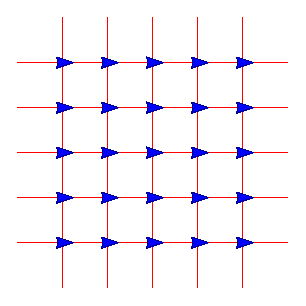
\includegraphics[trim=0.5cm 0.5cm 0.5cm 0.5cm, clip=true]{figs/sq-lat}
    \end{minipage}
    \caption{[left] A lattice graph representing a repeated square
    pattern. There is one node with four outgoing edges connecting to
    itself. Here the edge length is $1$. For a robot playing the role
    of this node, its neighbors should be in locations $(1, 0), (0,
    -1), (-1, 0)$ and $(0, 1)$, with the same orientation. [right]
    A repeated square lattice pattern represented by the left
    graph.}
    \label{fig:sq}
\end{figure}
%%%%%%%%%%%%%%%%%%%%%%%%%%%%%%%%%%%%%%
\begin{figure}
    \centering
    \begin{minipage}[b]{0.45\linewidth}
        \centering
        
    \begin{tikzpicture}[->,>=stealth',shorten >=5pt,auto,node distance=3cm]
      \tikzstyle{every state}=[draw=none]
      \node[state, scale=0.7, fill=red!50] (A) at (0,0)    {$0$};
      \node[state, scale=0.7, fill=blue!50] (B) at (3,0)  {$1$};
      \path (A) edge [bend left=10] node {\scriptsize{(0, 40,0)}} (B)
            (A) edge [bend left=45] node {\scriptsize{(-35,-20,0)}} (B)
            (A) edge [bend left=90] node {\scriptsize{(35,-20,0)}} (B)
            (B) edge [bend left=10] node {\scriptsize{(-40,0,0)}} (A)
            (B) edge [bend left=45] node {\scriptsize{(35,20,0)}} (A)
            (B) edge [bend left=90] node {\scriptsize{(-35,20,0)}} (A);
    \end{tikzpicture}
  
    \end{minipage}
    \begin{minipage}[b]{0.45\linewidth}
        \centering
        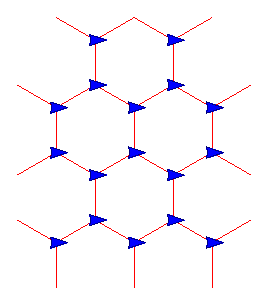
\includegraphics[scale=0.85]{figs/hex-lat}
    \end{minipage}
    \caption{[left] A lattice graph representing a repeating hexagon lattice pattern on the right. In the graph, the edge length is $40$. For a robot playing the role vertex $0$, its neighbors should be in locations $(35, -20), (-35, -20)$ and $(0, 40)$ with the same headings, and its neighbors should play the role vertex $1$ which has outgoing edges to vertex $0$. [right] A repeating hexagon lattice pattern represented by the left graph.}
    \label{fig:hex}
\end{figure}
%%%%%%%%%%%%%%%%%%%%%%%%%%%%%%%%%%%%%%
\begin{figure}
    \centering
    \begin{minipage}[b]{0.45\linewidth}
        \centering
        \begin{tikzpicture}[->,>=stealth',shorten >=5pt,auto,node distance=1.5cm]
    \tikzstyle{every state}=[fill=red!50, draw=none]
            %                  D
            %      C      A 
            % 
            %             B
        \node[state, scale=0.7] (A) at (0,0)    {$0$};
        \node[state, scale=0.7, fill=cyan] (B) at (0,-2)  {$1$};
        \node[state, scale=0.7, fill=blue!50] (C) at (-2,0) {$2$};
        \node[state, scale=0.7, fill=orange] (D) at (1,1) {$4$};
        \path (A) edge (B)% node {\scriptsize{Tr(0, -40)}} (B)
              (A) edge (C) %node {\scriptsize{Tr(-40, 0)}} (C)
              (A) edge (D); %node {\scriptsize{Tr(28,28)}}  (D);
        \path (B) edge [bend left=10] (A)
              (B) edge (D) % node {\scriptsize{Tr(-40,0)}}  (D); 
              (B) edge (C);% node {\scriptsize{Tr(-28,28)}} (C);
        \path (C) edge [bend right=30] (B)
              (C) edge [bend left=10] (A)
              (C) edge [bend left=30] (D);
        \path (D) edge [bend left=30] (B)
              (D) edge [bend right=10] (A)
              (D) edge (C);
\end{tikzpicture}
    \end{minipage}
    \begin{minipage}[b]{0.45\linewidth}
        \centering
        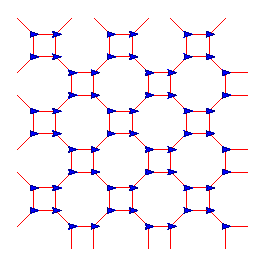
\includegraphics[scale=0.95]{figs/octsq-lat}
    \end{minipage}
    \caption{[left] A lattice graph representing a repeating octagon-square lattice pattern on the right (for simplicity, we do not show the edges' transformations). [right] A repeating octagon-square lattice pattern represented by the left graph.}
    \label{fig:octagonsquare}
\end{figure}
%%%%%%%%%%%%%%%%%%%%%%%%%%%%%%%%%%%%%%

\begin{defn}
  Given a lattice graph $G=(V, E)$ and a set of robots
    $R = \{ r_1, \ldots, r_n \}$,
  we say that $R$ \textbf{satisfies} $G$ if there exists a function
    $f: R \rightarrow V$
  that preserves the neighborhood structure of $G$.
  %
  Specifically, for any $i$ and $j$, if $r_i$ and $r_j$ are neighbors, 
  there must exist an edge
  $e_v^w: \edge{f(r_i)}{}{f(r_j)}$ in $E$, such that 
      $f(r_i) = v$,
      $f(r_j) = w$, and $T(r_j) = T(r_i) T(e_{v}^w)$.
\end{defn}

\subsection{Lattice Graph Constraint}
However, the graph definition of a lattice may describe some geometric patterns contradicting themselves. To guarantee a pattern is represented properly using a lattice graph, we define a constraint, termed ``self-consistent'', for a lattice graph, so that the represented pattern will not contradict itself by forcing pairs of robots to be mutual neighbors, with roles that are not adjacent in the lattice graph. 
%
Figure~\ref{fig:self-consistent-graph} shows a comparison between a simple
lattice graph that is not self-consistent with one that is self-consistent.


\begin{defn}
  \label{def:selfconsistent}
  Given a range $\range > 0$, call a lattice graph \textit{self-consistent} for
  this range if, for any two paths with the same starting node,
  $$ \lgpath{v}{T(e_v^{k})}{T(e_m^{w})}{w}, \mbox{ and } 
    \lgpath{v}{T(e_v^{j})}{T(e_n^{u})}{u}, $$
  for which the distance between two ending nodes is less than or equal to
  $\range$, there exist edges between $w$ and $u$.
\end{defn}


%%%%%%%%%%%%%%%%%%%%%%%%%%%%%%%%%%%%%%%%
\begin{figure}
    \centering
     \begin{minipage}[b]{0.4\linewidth}
  \centering
  \begin{tikzpicture}[scale=1.2]
    \tikzstyle{every state}=[fill=red!50, draw=none]
    \node[state, scale=0.7] (A) at (2.5,0)    {\large{$u$}};
    \node[state, scale=0.7] (C) at (0, 0.75) {\large{$w$}};
    \node[state, scale=0.7] (D) at (0, -0.75) {\large{$z$}};
    \draw[arc] (A) to[out=150, in=0] (C);
    \draw[arc] (A) to[out=-150,in=0] (D);
    \draw[arc] (C) to[out=-30, in=170] (A);
    \draw[arc] (D) to[out=30, in=-170] (A);
    \node[] at (0.8, -1.2) {\scriptsize{$\left(0, l, 0\right)$}};
    \node[] at (0.8, 1.2) {\scriptsize{$\left(\dfrac{l}{2}, l, 0\right)$}};
    %\node[] at (-0.5, 0) {\scriptsize{$(\dfrac{\range}{2}, 0, 0)$}};
  \end{tikzpicture}
  \end{minipage}
  \begin{minipage}[b]{0.5\linewidth}
    \centering
    \begin{tikzpicture}[scale=1.2]
       \tikzstyle{every state}=[fill=red!50, draw=none]
       \node[state, scale=0.7] (A) at (2.5,0)   {\large{$u$}};
       \node[state, scale=0.7] (C) at (0, 0.75) {\large{$w$}};
       \node[state, scale=0.7] (D) at (0, -0.75) {\large{$z$}};
       \draw[arc] (A) to[out=150, in=0] (C);
       \draw[arc] (A) to[out=-150,in=0] (D);
       \draw[arc] (C) to[out=-30, in=170] (A);
       \draw[arc] (D) to[out=30, in=-170] (A);
       \draw[arc] (C) to[out=-60, in=60] (D);
       \draw[arc] (D) to[out=120, in=-120] (C);
       \node[] at (0.8, -1.2) {\scriptsize{$\left(0, l, 0\right)$}};
       \node[] at (0.8, 1.2) {\scriptsize{$\left(\dfrac{l}{2}, l, 0\right)$}};
       \node[] at (-1, 0) {\scriptsize{$\left(\dfrac{l}{2}, 0, 0\right)$}};
    \end{tikzpicture}
  \end{minipage}
  \caption{[left] A lattice graph that is not self-consistent when $\range > l$.
  The distance between robots with roles $w$ and $z$ is less than
  $l/2 < \range$, but no edge connects $w$ and $z$.  [right] A lattice graph
  that is self-consistent when $\range > l$.} 

    \label{fig:self-consistent-graph}
\end{figure}
%%%%%%%%%%%%%%%%%%%%%%%%%%%%%%%%%%%%%%%%


Meanwhile, the self-consistent property is an important constraint for our algorithm to generate correct output.

%%%%%%%%%%%%%%%%%%%%%%%%%%%%%%%%%%%%%%%%
\begin{figure}
    \centering
    \begin{minipage}[b]{0.45\linewidth}
    \centering
    \begin{tikzpicture}[->,>=stealth',node distance=5cm]
      \tikzstyle{every state}=[fill=red!50,draw=none]
      \node[state, scale=0.7] (A)    {$0$};
      \path (A) edge [loop right] node {\footnotesize{(1, 0, $45^\circ$)}} (A)
                edge [loop left] node {} (A); %{\footnotesize{(-1,0,$45^\circ$)}} (A);
    \end{tikzpicture}
  \end{minipage}    
%   \begin{minipage}[b]{0.5\linewidth}
%     \centering
%     \begin{tikzpicture}
%     \draw[fill=blue] (3,2.92) -- (2.5,2.75) -- (3,2.58) -- (2.875,2.75) -- cycle;
%     \draw[fill=blue] (2,2.92) -- (1.5,2.75) -- (2,2.58) -- (1.875,2.75) -- cycle;
%     \draw[fill=blue] (1,2.92) -- (0.5,2.75) -- (1,2.58) -- (0.875,2.75) -- cycle;
%     \draw[dashed](2.5,2.75) -- (1.5,2.75);
%     \draw[dashed](1.5,2.75) -- (0.5,2.75);
%     \draw[dashed](0.5,2.75) -- (-0.5,2.75);
%     \draw[dashed](2.5,2.75) -- (4,2.75);
%   \end{tikzpicture}
%   \end{minipage}
   \begin{minipage}[b]{0.45\linewidth}
     \centering
     \begin{tikzpicture}[->,>=stealth',node distance=5cm]
       \tikzstyle{every state}=[fill=red!50,draw=none]
       \node[state, scale=0.7] (A)    {$0$};
       \path (A) edge [loop right] node {\footnotesize{(0, 1, $45\sqrt{2}^\circ$)}} (A)
                 edge [loop left] node {} (A); %{\footnotesize{(0, -1, $-45\sqrt{2}^\circ$)}} (A);
     \end{tikzpicture}
 \end{minipage}
 \caption{[left] A self-consistent lattice graph. 
            [right] A non-self-consistent lattice graph.}

\end{figure}
%%%%%%%%%%%%%%%%%%%%%%%%%%%%%%%%%%%%%%%%

Figures~\ref{fig:lg1}, \ref{fig:lat1} and \ref{fig:lg2} illustrate another example of a comparison between a self-consistent lattice graph and a lattice graph that is not self-consistent. 
%
For the range we assume $1 < \range < \sqrt{2}$, 
the graph in Figure~\ref{fig:lg1} contains a node with two out-going edges, on the above edge, we apply rotation of $90^{\circ}$ and translation $(0, 1)$ in order to get the adjacent pose; whereas on the below edge, we apply translation of $(0, -1)$ and then rotation of $-90^{\circ}$ to get the other adjacent pose. 
%
Figure~\ref{fig:lat1} shows four robots at positions satisfying the
lattice graph in Figure~\ref{fig:lg1}. 

Similar to the graph in Figure~\ref{fig:lg1}, but we apply the rotation of $45\sqrt{2}^{\circ}$ to the out-going edges, then we obtain a non-self-consistent lattice graph in Figure~\ref{fig:lg2} representing a whirlpool-like repeated pattern.

% It is not practical to verify a self-consistent lattice graph in terms of the
% Definition~\ref{def:selfconsistent}, that is, simply using a brute force method
% to track every path and compare the distance between two terminal nodes of two
% paths with the given range. For example, there are infinite paths in the lattice
% graphs shown in Figures~\ref{fig:lg1} and \ref{fig:lg2}.  We observe that the
% graph in Figure~\ref{fig:lg1} produces a single square lattice in which from any
% vertex of the square, we can always find a path whose ending node corresponds
% the same position as the staring vertex of this lattice.  However, the graph in
% Figure~\ref{fig:lg2} produces a lattice in which from any vertex's position, we
% would find a path that ends at the position where the distance to the starting
% vertex is less than the given range.

%\clearpage
\section{Evaluation Criteria}
\label{sec:mrf-eval}

To verify the effectiveness of our algorithms, we have designed two evaluation criteria so that we could run simulations to collect the measurements.

\subsubsection{Execution time}
The first measurement we concern is the time needed for the robots to reach static positions.

\begin{defn}
A robot $r_i$ is \textbf{static} at time $t$ if its pose $p_i$
remains the same at all future times, so that 
  \begin{equation}
    p_i(t') = p_i(t) \quad \mbox {for all } t' > t.
  \end{equation}
\end{defn}

Define the \textbf{execution time} $\Time$ of the system as the smallest time when all the robots reach in static states:
\begin{equation}
  \Time = \inf \{t \in (0, \infty) \mid \mbox{every $r \in R$ stays static
    after time $t$ } \}
\end{equation}

Smaller execution time indicates more efficient computation, so we desire $\Time$ as small as possible.

\subsubsection{Formation fulfillment Ratio}

The second measurement is the quality of the finally formed pattern.
%
After all robots reach static positions, for a robot $r_i$
with $E_i$ outgoing edges from its role vertex, 
namely, the maximum number of neighbors it could have in order to form the desired lattice represented by given lattice graph, if the actual number of neighbors it has is $N_i$, 
we evaluate the overall lattice quality by a fulfillment ratio:
\begin{equation}\label{eq:gamma}
  \Quality = \dfrac{1}{n}\sum\limits_{i=1}^n \frac{N_i}{E_i}
\end{equation}

The ratio $\Quality \in [0, 1]$ approximately reflects how satisfactory the final formation is with regard to the given lattice graph. 
%
We prefer a formation with a value of $\Quality$ as large as possible.

Figure~\ref{fig:hex-qual} shows that both sets of robots satisfy the lattice
graph in Figure~\ref{fig:hex} but with different fulfillment ratios.
\begin{figure}  
    \centering
    \begin{minipage}[b]{0.95\linewidth}
        \centering
        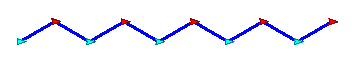
\includegraphics[width=0.75\textwidth]{figs/bad-hexagon}
        
    \end{minipage}
    \begin{minipage}[b]{0.95\linewidth}
        \centering
        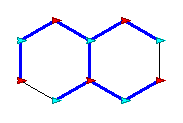
\includegraphics[width=0.3\textwidth]{figs/good-hexagon}
    \end{minipage}
    \caption{Possible formations of $10$ robots satisfying the hexagon lattice graph. [top] Fulfillment ratio $\Quality=0.6$. 
    [bottom] Fulfillment ratio $\Quality = 0.733$.}
    \label{fig:hex-qual}
\end{figure}


\chapter{Task-Assignment-based Formation Algorithm}
\label{chp:mrf1}
In this chapter, we introduce our first novel distributed solution. 
%
The key idea of our method is enabling robots to construct a global structure to
organize themselves using only local information, so that we can have the
desired lattice formed by deploying local task assignment strategy in the system. 
%
Our approach presented in this chapter include mainly two novelties: (1) A
global structure to organize robots (``authority tree'') and (2) a distributed
control strategy for robots to form the desired pattern.


%We describe a scalable formation algorithm in this chapter. 
%
The remaining sections of this chapter are organized as follows. 
%
Section~\ref{sec:msg1} describes the important terminology of ``authority'' used in this algorithm.
The details of the algorithm are described in Section~\ref{sec:auth} and Section~\ref{sec:task-assgin-algo}, including the
procedure of the authority tree construction and local task assignment deployment. 
%
In Section~\ref{sec:mrf-exp}, we evaluate our algorithm through simulations, 
and evaluate the effectiveness of our algorithm based on the experimental results. 
%
Finally, Section~\ref{sec:conc-mrf1} lists the advantages and disadvantages of the algorithm. 
Furthermore, the limitations of this algorithm motivate us to extend our work on the formation problem and contribute a new method described in Chapter~\ref{chp:mrf2}.

%\clearpage
\section{Robot Communication}
\label{sec:msg1}
An important feature of this distributed formation algorithm is that it is stateless.
%
Each robot makes movements and constructs messages to broadcast based on its recent observations and received messages.
%
With this design, our algorithm is robust to the scenarios when some robots fails to react with others or some new robots are added to the system.

Robots coordinate with their neighbors by exchanging messages. 
%
Each robot periodically broadcasts a message containing:
  \begin{enumerate}
  \item An \textbf{authority} -- the level of importance of the sender robot (see Section~\ref{sec:auth}).
  \item A \textbf{role} -- an integer identifying a lattice graph vertex as the role currently selected by the sender robot.
  \item A \textbf{matching} of the neighbors of the sender robot to outgoing edges of its
  role vertex, or to a dummy ``no-match'' element.
 \end{enumerate}

Section~\ref{sec:auth} discusses the details of building a global tree structure using the authorities delivered in local neighbors' messages.
% 
The role is the key information for each robot to execute local task-assignment,
%
whereas, the matching is the output of the task-assignment.
%
Section~\ref{sec:task-assgin-algo} presents the procedure of assigning local tasks.

%\clearpage
\section{Authority}
\label{sec:auth}

Our method takes advantage of the task assignment problem.
A key idea is to determine the local ``leader'' that assigns tasks among nearby robots. 
%
Unlike prior work applying the auction-based strategies for task assignment~\cite{Ber88, FarIocNarZip06, ZavSpePap08, MicZavKumPap08, ChoBruHow09, ChaHenIAS13, LiuShe13}, 
our work contributes to produce a stable structure for robots to do the 
task assignment without multiple iterations of bidding for tasks.


The idea to make our local strategy reach a global static state is the authority carried by each robot.  
%
First, we define the term ``authority'' and its associated comparison operation, 
then we describe the algorithm for the robots to construct a tree structure using these authorities.

\begin{defn}
  An \textbf{authority} is an ordered list of robot IDs
    $$\L = \langle \id_1, \ldots, \id_k \rangle,$$
   which contains
    \begin{enumerate}
    \item \textbf{root} ID: The first ID in the list, $\id_1$;
    \item \textbf{sender} ID: The final ID in the list, $\id_k$;
    \item \textbf{length}: Number of IDs in the list.
    \end{enumerate}
\end{defn}

\begin{defn}
  Given two authorities
    $\L_1=\langle \id_1^1, \ldots, \id_k^1\rangle$
  and
    $\L_2=\langle \id_1^2, \ldots, \id_l^2\rangle$,
  $\L_2$ is \textbf{higher than} $\L_1$ if 
  \begin{enumerate}
    \item $\id_1^2 > \id_1^1$, or
    \item $l < k$ if $\id_1^2 = \id_1^1$, or
    \item $\id_l^2 > \id_k^1$, if $\id_1^2 = \id_1^1$ and $l = k$.
  \end{enumerate}
\end{defn}


Initially each robot creates its authority containing only its own ID. 
%
After exchanging messages, robot selects the neighbor whose message contains the highest authority among all of its neighbors and has matching
(Definition~\ref{def:matching}) with it as its parent. 
%
Otherwise, the robot considers itself a \textbf{root} robot. 
%
Meanwhile, non-root robots select their parents, if any, and the neighbors with the highest IDs less than its own as \textbf{descendant} candidates to form matching. 
%
The number of neighbors selected to form matching does not exceed the out-degree of the robot's role. 
%
The descendant robot produces an authority to transmit with its next message by appending its own ID to the authority of its parent. 
%
If a robot is not matched by every neighbor who has higher authority than its own, than it is an \textbf{orphan} robot (Figure~\ref{fig:orphan}).
%%%%%%%%%%%%%%%%%%%%%%%%%%%%%%%%%%%%%%%%
\begin{figure}
  \centering
  
\includegraphics[scale=0.75]{figs/sq17}
  \caption{All red robots have matching with red neighbors around, given input square lattice graph.
           The green robot has no matching with any neighbor, thus it is an orphan robot.}
    \label{fig:orphan}
\end{figure}
%%%%%%%%%%%%%%%%%%%%%%%%%%%%%%%%%%%%%%%%

Additionally, to avoid creating an authority tree with cycle, each robot ignores any authority that already contains its own ID.
%
Figure~\ref{fig:authtree} shows a simple case when constructing the authority tree.
%%%%%%%%%%%%%%%%%%%%%%%%%%%%%%%%%%%%%%%%
\begin{figure}
  \begin{minipage}[b]{0.45\linewidth}
    \centering
    \begin{tikzpicture}[scale=1.25]
      \draw[fill=blue!50] (3.2,2.5) -- (2.95,2.5) -- (3.45,2.75) -- (3.2,2.25)   -- cycle;
      \node[color=blue] at (3.2, 2) {$r_2$};
      % draw grids
      % \draw[color=gray, help lines, line width=.05pt] (-1,1)  grid[xstep=.5cm, ystep=.5cm] (6,6);
      \draw[fill=blue!50] (3,4.5) -- (2.75,5) -- (2.75,4.75) -- (2.5,4.75)   -- cycle;
      \node[color=blue] at (3.25, 5) {$r_0$};
      \draw[fill=blue!50] (5.2,3.42) -- (4.7,3.25) -- (5.2,3.08) -- (5.075,3.25)  -- cycle;
      \node[color=blue] at (5.4,3.25) {$r_1$};    
      \draw[fill=red] (4,4) -- (3.75,4) -- (4.25,4.25) -- (4,3.75) -- cycle;
      \node[color=red] at (4, 3.5) {$r_3$};
      \draw[color=red] (3,4) -- (2.75,4) -- (3.25,4.25) -- (3,3.75) -- cycle;
      \draw[dashed] (3,4) -- (4,4);
      % \draw (0,-4.75) node[below] {reflect across $x$-axis};  
      \draw[color=red] (5,4) -- (4.75,4) -- (5.25,4.25) -- (5,3.75) -- cycle;
      \draw[dashed] (5,4) -- (4,4);
    \end{tikzpicture}
  \end{minipage}
  \begin{minipage}[b]{0.45\linewidth}
    \centering
    \begin{tikzpicture}[scale=1.25]
      \node[] (A) at (4,4)    {$\langle3\rangle$};
      \node[] (B) at (3,2.5)  {$\langle2\rangle$};
      \node[] (C) at (5.5,4)  {$\langle3,1\rangle$};
      \node[] (D) at (3,5)    {$\langle3,0\rangle$};
      \draw[edge] (A) -- (D);
      \draw[edge] (A) -- (C);
    \end{tikzpicture}
  \end{minipage}
  \caption{[left] A root robot $r_3$ has three neighbors, and two outgoing
  edges from its role vertex.  [right] After exchanging messages. Robot $r_3$ selects $r_0$ and $r_1$ as its children since they are two robots who are closest to two desired opening position corresponding to the out-edges. Robot $r_2$ is an orphan without any assignment.}
  \label{fig:authtree}
\end{figure}
%%%%%%%%%%%%%%%%%%%%%%%%%%%%%%%%%%%%%%%%

%\clearpage
\section{Distributed Task-Assignment}
\label{sec:task-assgin-algo}

In this section, we describe the primary version of our formation algorithm. 
%
The algorithm takes the lattice graph as an input to form the desired lattice pattern. 
%
Generally, each robot repeats following steps every $\dt$ seconds:
\begin{enumerate}
\item Step 1: Robots use the matching contained in received messages to
  construct an authority tree based on their IDs.
\item Step 2: Each robot decides its ``role'', which is essentially a vertex in the lattice graph, it will play in the formation.  
    %
    The root of the authority tree selects the first vertex in the lattice graph as its role; 
    the descendant robots in the authority tree accept their roles as part of the task assignment from their parents. 
\item Step 3: Each robot finds a position, if any, where no robot is assigned and located, as the opening position it knows.
\item Step 4: Each robot computes a certain number of destinations in its body frame to
  assign its matching neighbors, using the standard Hungarian
  algorithm~\cite{Kuh55}. 
  %
  Each robot broadcasts a message containing its assignment, along with the authority value, and the opening position, if any, to its neighbors.
\item Step 5: Each robot computes its destination based on the assigned task and moves toward to the assigned destination according the motion strategy discussed in Section~\ref{sec:motion}.
\end{enumerate}

\subsection{Task Assignment}
\label{subsec:task}


Once the authority tree has been constructed, each root robot selects the first vertex of the lattice graph as its role; the descendant robots accept roles from their parents.

For a robot $r_i$ which has already selected its role, it needs to establish a
relationship, called \textbf{matching} between its neighbors and the outgoing edges from its role vertex. 
\begin{defn}
\label{def:matching}
  Given a robot $r_i$ and a role vertex $u$ for that robot, the lattice
  graph edge set
    $O=\{\emptyset, e_{u}^w, e_{u}^z, \ldots\}$
  contains a null value $\emptyset$ and all outgoing edges from vertex $u$.  
  Set
    $I=\{\id_a, \id_b, \ldots \}$
  contains the IDs of the neighbors of $r_i$.  
  Then a
  \textbf{matching for $r_i$} is a function $g : I \rightarrow O$ that
  associates each neighbor ID with either a lattice graph edge from its role vertex or with the null value.
\end{defn}

For example, in Figure~\ref{fig:authtree}, robot $r_2$ is an orphan robot to the root robot $r_3$, with $g(\id_{r_2}) = \emptyset$.

Assume that robot $r_i$ has $N_i$ neighbors and its out-degree is $E_i$. 
%
We interpret this problem as a task assignment problem~\cite{Kuh55, Mun57}: 
Given $\min(N_i, E_i)$ agents and $E_i$ tasks, we create a $\min(N_i, E_i)\times E_i$ matrix containing the cost of assigning each agent to a task. 
%
The goal is finding the cost minimizing assignment. 
%
(The number of agents is not greater than the number of
the out-degree since a parent robot always selects maximum $E_i$ neighbors as to form matching with it).

Specifically, in the cost matrix, each row corresponds to an ID of a non-orphan neighbor of $r_i$, and each column corresponds to an outgoing edge from its role $f(r_i)$. 
%
We define the cost as the Euclidean distance for a neighbor robot to
travel from its current position $(x^{(i)}, y^{(i)})$ to the desired
position $(\bar{x}^{(i)}, \bar{y}^{(j)})$. 
%
%TODO: replace transformation T with \math font, consistent with RAL
Given an edge $e$, we can use its transformation $\Tr(e)$ to find the desired position.
\begin{equation}
  \label{eq:trans-pos}
  \left[\bar{x}^{(i)} \quad \bar{y}^{(i)} \quad 1\right]^\top = \Tr(e) \left[0 \quad 0 \quad 1\right]^\top
\end{equation}

The procedure to construct the cost matrices for a root robot and a descendant robot are slightly different.

\subsubsection{Root Matching}

For a root robot $r_i$, in its cost matrix:
\begin{enumerate}
  \item Each row of the matrix corresponds to a neighbor of $r_i$;
  \item each column of the matrix corresponds to an out-edge of $f(r_i)$;
  \item the entry of the matrix in row $j, j \in [1, \min(N_i,\ldots, E_i)]$, column
    $k, k \in (1,\ldots, E_i)$ represents the Euclidean distance $|| \bar{p}_j^{(i)} -
    {p}_j^{(i)} ||$ between the current position of the $j^{th}$ neighbor and
    its desired position if matched with the $k^{th}$ outgoing edge (both computed in the body frame of $r_i$).  
\end{enumerate}

We apply the Hungarian algorithm~\cite{Kuh55} to solve the assignment problem. 
%
Each robot executes the Hungarian algorithm on the cost matrix
to compute matching of its neighbors to its outgoing edges, by minimizing the total Euclidean distance. 
%
The algorithm takes $O(N_i^3)$ time complexity.

%
In Figure~\ref{fig:formsquare}, the center robot, which is a root, finds matching for four of its
neighbors and assign them to desired poses in its body frame, meanwhile, there
is no matching found for one of its neighbors.
%%%%%%%%%%%%%%%%%%%%%%%%%%%%%%%%%%%%%%%%%%%%%%
\begin{figure}
    \centering
    \begin{minipage}{0.9\textwidth}
    \centering
      \begin{tikzpicture}[scale=1.25]
    \draw[fill=red] (3,3) -- (2.75,3) -- (3.25,3.25) -- (3,2.75) -- cycle;
    \node[color=red] at (3, 2.5) {$r_6$};
    %\draw[thick, ->] (-1,0) -- (6,0) node[right] {X};
    %\draw[thick, ->] (0,-1) -- (0,6) node[above] {Y};
    \draw[color=red, dashed, ->] (1.5,1.5) -- (5,5) node[right] {$X^{(r_6)}$};
    \draw[color=red, dashed, ->] (4.5,1.5) -- (1,5) node[above] {$Y^{(r_6)}$};
    % draw grids
    %\draw[color=gray, help lines, line width=.05pt] (-1,1)  grid[xstep=.5cm, ystep=.5cm] (6,6);
    \draw[fill=blue!50] (0.5,4.5) -- (0.33,4) -- (0.5,4.125) -- (0.67,4)    -- cycle;
    \node[color=blue] at (0.5,3.75) {$r_2$};
    \draw[fill=blue!50] (4,5) -- (3.75,5.5) -- (3.75,5.25) -- (3.5,5.25)        -- cycle;
    \node[color=blue] at (3.5,5.7) {$r_5$};
    \draw[fill=blue!50] (1,2.5) -- (1.25,2) -- (1.25,2.25) -- (1.5,2.25)        -- cycle;
    \node[color=blue] at (1.2,1.7) {$r_4$};
    \draw[fill=blue!50] (5,2.92) -- (4.5,2.75) -- (5,2.58) -- (4.875,2.75)  -- cycle;
    \node[color=blue] at (5.4,2.75) {$r_3$};
%    \draw[fill=blue!50] (2.5,0) -- (2.7,0.52) -- (2.5,0.35) -- (2.3,0.52)   -- cycle;
%    \node[color=blue] at (2.5,0.75) {$r_1$};
    \draw[fill=orange!50] (-0.5,2.5) -- (-0.5,2.75) -- (-0.75,2.25) -- (-0.25,2.5)  -- cycle;
    \node[color=blue] at (-0.75,3) {$r_1$};
        
    \draw[color=red] (4,4) -- (3.75,4) -- (4.25,4.25) -- (4,3.75) -- cycle;
    \draw[color=red] (2,2) -- (1.75,2) -- (2.25,2.25) -- (2,1.75) -- cycle;
    \draw[color=red] (2,4) -- (1.75,4) -- (2.25,4.25) -- (2,3.75) -- cycle;
    \draw[color=red] (4,2) -- (3.75,2) -- (4.25,2.25) -- (4,1.75) -- cycle;
        
    \draw[dashed](0.5, 4.125) -- (2,4);
    \draw[dashed](1.25,2.25) -- (2,2);
    \draw[dashed](3.75,5.25) -- (4,4);
    \draw[dashed](4.875,2.75) -- (4,2);
%   \draw (0,-4.75) node[below] {reflect across $x$-axis};  
  \end{tikzpicture}
    \end{minipage}
    \caption{Matching computed by the root robot $r_6$.}
    \label{fig:formsquare}
\end{figure}
%%%%%%%%%%%%%%%%%%%%%%%%%%%%%%%%%%%%%%%%%%%%%
\begin{figure}
    \centering
    \begin{tikzpicture}[scale=1.5]
    \node[] (I) at (3,3)   {$\langle6\rangle$};
    \node[] (B) at (0,2)   {$\langle6,4,1\rangle$};
    \node[] (C) at (2,4)   {$\langle6,2\rangle$};
    \node[] (D) at (4,2)   {$\langle6,3\rangle$};
    \node[] (E) at (2,2)   {$\langle6,4\rangle$};
    \node[] (F) at (4,4)   {$\langle6,5\rangle$};
    
    \draw[edge] (I) -- (C);
    \draw[edge] (I) -- (D);
    \draw[edge] (I) -- (E);
    \draw[edge] (I) -- (F);
    \draw[edge] (E) -- (B);
\end{tikzpicture}
\caption{Authority tree constructed by the robots in Figure~\ref{fig:formsquare}.}
    \label{fig:formsquare-auth}
\end{figure}
%%%%%%%%%%%%%%%%%%%%%%%%%%%%%%%%%%%%%%%%%%%%%%

\subsubsection{Descendant Matching}

Similar to the process of computing matching for the root robot, the steps to compute matching for a descendant robot are identical except for two differences:
\begin{enumerate}
\item A descendant robot chooses its role according to the matching received from its parent.  
%
    Specifically, the role of a descendant is the terminal vertex of
  the edge associated with its own ID in that matching. 
\item A descendant robot, in its matching, ensures that the parent is
  matched with the outgoing edge, whose transformation is the inverse of the edge matching it.
\end{enumerate}

Figure~\ref{fig:formsquare} shows the procedure of computing the matching by a root robot and a descendant robot, respectively. 
%
Given an input lattice graph in Figure~\ref{fig:sq}, robot $r_6$ has $5$ neighbors $r_1, r_2, r_3, r_4, r_5$; robot $r_4$ has three neighbors $r_6, r_2, r_1$. 
%
By exchanging messages, the authority tree constructed by the robots is shown in Figure~\ref{fig:formsquare-auth}.
%
Then $r_6$ is a root and it chooses the first vertex of the lattice graph as its role.
%
The root robot $r_6$ computes four desired positions in its body frame according to the cost matrix for its descendants.
%
Robot $r_1$ is too far away to be selected by $r_6$ to form matching, so it is an orphan (Figure~\ref{fig:formsquare}).
%
On the other side, robot $r_4$ recognizes itself as a descendant of the root $r_6$.
%
It first computes its own matching for its neighbors, $r_6, r_2, r_1,$ in its local frame. 
%
However, $r_4$ must force its matching with $r_6$ to be consistent with $r_6$'s matching with it.
%
Recall that $r_6$ already assigns a role vertex to $r_4$, which corresponds to the position behind the root $r_6$ (the red hollow arrow in Figure~\ref{fig:formsquare-des}).
%
Therefore, $r_4$ finds the reverse edge with a terminal node matching that destination in its own coordinate frame, that is, the position in front of it. 
%
Then it matches the root to this edge with itself and computes the local optimal matching for the rest of its neighbors $r_2, r_1$.

%%%%%%%%%%%%%%%%%%%%%%%%%%%%%%%%%%%%%%%%%%%%%%
\begin{figure}
    \centering
    \begin{minipage}{0.9\textwidth}
    \centering
    \begin{tikzpicture}[scale=1.5]
    \draw[fill=red] (3,3) -- (2.75,3) -- (3.25,3.25) -- (3,2.75)        -- cycle;
    \node[color=red] at (3, 2.5) {$r_6$};
    %\draw[thick, ->] (-1,0) -- (6,0) node[right] {X};
    %\draw[thick, ->] (0,-1) -- (0,6) node[above] {Y};
    % draw grids
    %\draw[color=gray, help lines, line width=.05pt] (-1,1)  grid[xstep=.5cm, ystep=.5cm] (6,6);
    % center of rc : 0.5, 4.125
    \def\Cx{0.5}
    \def\Cy{4.125}
    \def\d{1.5}
    \def\dd{1}
    \coordinate (C) at (\Cx, \Cy);
    \def\Ex{1.25}
    \def\Ey{2.25}
    \coordinate (E) at (\Ex, \Ey);
    \draw[color=blue, dashed, ->] (\Ex+\d, \Ey+\d) -- (\Ex-\d,\Ey -\d) node[right] {$Y^{(r_4)}$};
    \draw[color=blue, dashed, ->] (\Ex +\d,\Ey-\d) -- (\Ex -\d,\Ey+\d) node[above] {$X^{(r_4)}$};
    \draw[fill=blue!50] (0.5,4.5) -- (0.33,4) -- (C) -- (0.67,4) -- cycle;
    \node[color=blue] at (0.5,3.75) {$r_2$};
    \draw[fill=blue!50] (4,5) -- (3.75,5.5) -- (3.75,5.25) -- (3.5,5.25)  -- cycle;
    \node[color=blue] at (3.5,5.7) {$r_5$};
    \draw[fill=blue] (1,2.5) -- (1.25,2) -- (E) -- (1.5,2.25)  -- cycle;
    \node[color=blue] at (1.2,1.7) {$r_4$};
    \draw[fill=blue!50] (5,2.92) -- (4.5,2.75) -- (5,2.58) -- (4.875,2.75)  -- cycle;
    \node[color=blue] at (5.4,2.75) {$r_3$};
    \draw[fill=orange!50] (-0.5,2.5) -- (-0.5,2.75) -- (-0.75,2.25) -- (-0.25,2.5)  -- cycle;
    \node[color=blue] at (-0.75,3) {$r_1$};
    \coordinate (I) at (3,3);
    \coordinate (B) at (-0.5, 2.5);
    \draw[color=blue] (1-\dd,2.5+\dd) -- (1.25-\dd,2+\dd) -- (\Ex-\dd, \Ey+\dd) -- (1.5-\dd,2.25+\dd)  -- cycle;
    \draw[color=blue] (1-\dd,2.5-\dd) -- (1.25-\dd,2-\dd) -- (\Ex-\dd,\Ey-\dd) -- (1.5-\dd,2.25-\dd)  -- cycle;
    \draw[color=blue] (1+\dd,2.5-\dd) -- (1.25+\dd,2-\dd) -- (\Ex+\dd, \Ey-\dd) -- (1.5+\dd,2.25-\dd)  -- cycle;
    \draw[color=blue] (1+\dd,2.5+\dd) -- (1.25+\dd,2+\dd) -- (\Ex+\dd,\Ey+\dd) -- (1.5+\dd,2.25+\dd)  -- cycle;
    
    \draw[color=red, dashed, ->] (1.5,1.5) -- (5,5) node[right] {$X^{(r_6)}$};
    \draw[color=red, dashed, ->] (4.5,1.5) -- (1,5) node[above] {$Y^{(r_6)}$};
    \draw[dashed](C) -- (\Ex+\dd, \Ey+\dd);
    \draw[dashed](B) -- (\Ex-\dd, \Ey-\dd);
    
    \draw[color=red] (2,2) -- (1.75,2) -- (2.25,2.25) -- (2,1.75) -- cycle;
    \draw[dashed](\Ex-\dd, \Ey+\dd) -- (I);
\end{tikzpicture}
    \end{minipage}
    \caption{Matching computed by the descendant robot $r_4$.}
    \label{fig:formsquare-des}
\end{figure}
%%%%%%%%%%%%%%%%%%%%%%%%%%%%%%%%%%%%%%%%%%%%%%

%\clearpage
\section{Motion Strategy}
\label{sec:motion}

Each robot determines its destination at the final step of the algorithm.  
%
We apply different moving plans for robots of different status:
\begin{enumerate}
\item Root -- the robot who has the highest authority among its neighbors -- does not move.
\item Descendant -- the robot who has a neighbor with higher authority and has matching with it -- moves toward assigned destination subject to Lemma~\ref{lem:boundedrange}.
\item Orphan -- the robot whose neighbors' authorities are higher but have no task assigned to it -- moves away from its current ``parent'' (the robot with the highest authority among its neighbors).
\end{enumerate} 


We assume that the robot can rotate infinitely fast, and provide a lemma to ensure the descendant robot remain in the range of its parent during its movement. 

Figure~\ref{fig:boundedrange} shows an example in which the actual
pose $p_p(t+\dt)$ of parent robot $r_p$ could be anywhere in the dotted
circle. 
%
At time $t$, robot $r_p$ assigns the desired goal pose $\bar{p}_i^{(p)}(t)$ to robot $r_i$.  
%
On the boundary of the intersection of $P_p \cap P_i$ (shaded area),
the nearest point to the desired ultimate destination position is
selected as the real goal position for $r_i$ at time $t+\dt$.

\begin{lem}
  \label{lem:boundedrange}
  If robot $r_i$ is the neighbor of robot $r_p$ at time $t$, it will still be the 
  neighbor of $r_p$ at time $t + \dt$ if $|| p_i(t+\dt) - p_p(t) || \leq \range -  v\dt$, where $v$ is the velocity of $r_i$ and $r_p$. 
\end{lem}

\begin{proof}
Because $r_i$ and $r_p$ are initially neighbors, we have
  \begin{equation}
    || p_i(t) - p_p(t) || \leq \range.
  \end{equation}
Due to the velocity limits on the robots, we also know that
  \begin{equation}\label{eq:d1}
    || p_p(t+\dt)- p_p(t) ||\leq v\dt.
  \end{equation}
since we assume that 
  \begin{equation}\label{eq:d2}
    || p_p(t) - p_i(t+\dt) || \leq \range - v\dt
  \end{equation}
then applying triangle inequality to Equation~\ref{eq:d1} and Equation~\ref{eq:d2} yields
  \begin{eqnarray*}
  \label{eq:d3}
    || p_p(t+\dt) - p_i(t+\dt) || & \leq || p_p(t+\dt) - p_i(t)|| \\
      & + || p_i(t) - p_i(t+\dt)|| \\
      & \leq \range - v\dt + v\dt = \range
  \end{eqnarray*}
\end{proof}
\begin{figure}
    \centering
      \def\firstcircle{(0,0) circle (2cm)}
  \def\secondcircle{(2.3,1.8) circle (1.5cm)}
  \def\thirdcircle{(0,0) circle (1.5cm)}
  \colorlet{circle edge}{blue!50}
  \colorlet{circle area}{blue!20}
  \tikzset{filled/.style={fill=circle area, draw=circle edge, thick},
    outline/.style={draw=circle edge, thick}}
  \tikzstyle{important line}=[very thick]
  \centering
  \begin{tikzpicture}
    \begin{scope}
        \clip \firstcircle;
        \fill[filled] \secondcircle;
    \end{scope}
    \draw[outline] \firstcircle node {$ $};
    \draw[fill=circle area] (0,0) circle (0.1cm); 
    \node at (-0.5,-0.3) {$p_p(t)$};
    \draw[style=important line, circle edge](90:1cm) -- node[black]{$\range- v\dt$}+(0,0);
   \draw[style=important line, circle edge](0,0) -- (135:2cm);
    \draw[outline] \secondcircle node {$ $};

    \draw[fill=circle area] (2.3,1.8) circle (0.1cm); 
    \node at (3.2, 2) {$p_i^{(p)}(t)$};

   \draw[style=important line, circle edge](2.3, 1.8) -- (1.55,3.09);
   \node at (1.5, 2.3) {$v\dt$};

    \draw[fill=circle area] (3, -0.7) circle (0.1cm); 
    \node at (3.8,-1) {$\bar{p}_i^{(p)}(t)$};
    \draw[dotted] \thirdcircle node{$ $};

   \draw[dotted](0, 0) -- (0,-1.5);
   \node at (0.5, -0.7) {$v\dt$};

  \draw[fill=circle area] (1.96, 0.32) circle (0.1cm); 
    \node at (3.5,0) {${p}_i^{(p)}(t+\dt)$};
  \end{tikzpicture}
  \caption{The real destination for the descendant robot $r_i$ to maintain connected with its parent $r_p$ during time $t+\dt$.}
    \label{fig:boundedrange}
\end{figure}

Lemma~\ref{lem:boundedrange} guarantees that a descendant robot always remains connected with its parent. 

An orphan robot is a special descendant who does not have an actual task assigned by its parent's matching, our motion plan simply drives the orphan robot away from its ``parent''. 
%
In detail, if the orphan robot receives a message from its parent, in which it is matched to $\emptyset$, it concludes that its current location is too congested.
%
In response, it moves directly away from its parent for a fixed period of time, equal to $2\range/v$.
%
The intuition is, we want the orphan robot to travel for a distance that is twice of its parent's range.
%
During this time, it does not communicate with anyone, and is neither root nor descendant. 
%
After this period, the orphan robot has a high possibility to move out of the range of its ``parent'' unless that ``parent'' moves towards the same direction as the orphan robot.
%
When this time expires, the robot resumes normal execution. 
%
The effect is to disperse the robots without oscillations, which could occur when the robot selects a new parent immediately afterward.


%\clearpage
\section{Experiments}
\label{sec:mrf-exp}
We have demonstrated the effectiveness of our algorithm using simulations implemented with C++. 
%
Recall that Figure~\ref{fig:octsq-init-final} shows a simulation result of forming the repeating octagon-square lattice pattern with $100$ robots.
%
We address an acknowledgement to Liu for his open-source contribution of the Hungarian algorithm implementation~\cite{LiuShe11, LiuShe12a}.


We conducted experiments to measure the algorithm execution time (the units of measurement are the simulation steps) and final lattice formation quality. 
%
Three types of repeating lattice patterns: hexagon (Figure~\ref{fig:hex}), square (Figure~\ref{fig:sq}), and octagon-square (Figure~\ref{fig:octagonsquare}) were used to test our algorithm.
%
For each lattice pattern, we performed a series of experiments, in which we varied the number of robots $n$ between $50$ and $250$ in increments of $50$.  
%
For each $n$, $50$ trials were tested with uniform distributions of initial poses randomly generated given distinct random seeds.

Figures~\ref{fig:octagonsquare-init-final}, \ref{fig:hex-init-final} and \ref{fig:sq-init-final} show the initial and final formations of three trials of simulations, whereas Table~\ref{tab:mrf1-exp-data} shows the corresponding results.
%
% In Figure~\ref{fig:octagonsquare-init-final}, the experiment took $\Time=1138$ simulation steps for $100$ robots to form a repeating octagon-square lattice pattern, with the fulfillment ratio $\Quality=0.694$.
% % 
% In Figure~\ref{fig:hex-init-final}, the experiment took $\Time=892$ simulation steps for $150$ robots to reach positions composing a repeating hexagon lattice pattern, with $\Quality=0.819$.
% %
% In Figure~\ref{fig:sq-init-final}, the experiment took $\Time=910$ simulation steps to form a repeating square pattern with $200$ robots, and the final fulfillment ratio $\Quality=0.725$.

\begin{table}
  \small\centering
  \caption{Experimental results of three trials of simulations.}
    \begin{tabular}{lccc} 
    \toprule 
    \textbf{Lattice Pattern} & \textbf{Number of Robots} & \textbf{Time (steps)} & \textbf{Fulfillment Ratio} \\
    \midrule
    Square & 200 & 910 & 0.725  \\ 
    \midrule
    Hexagon & 150 & 892 & 0.819 \\
    \midrule
    Octagon-Square & 100 & 1138 & 0.694 \\
    \bottomrule     
    \end{tabular}
    \label{tab:mrf1-exp-data}
\end{table}

%%%%%%%%%%%%%%%%%%%%%%%%%%%%%%%%%%%%%%%%
\begin{figure}
    \centering
   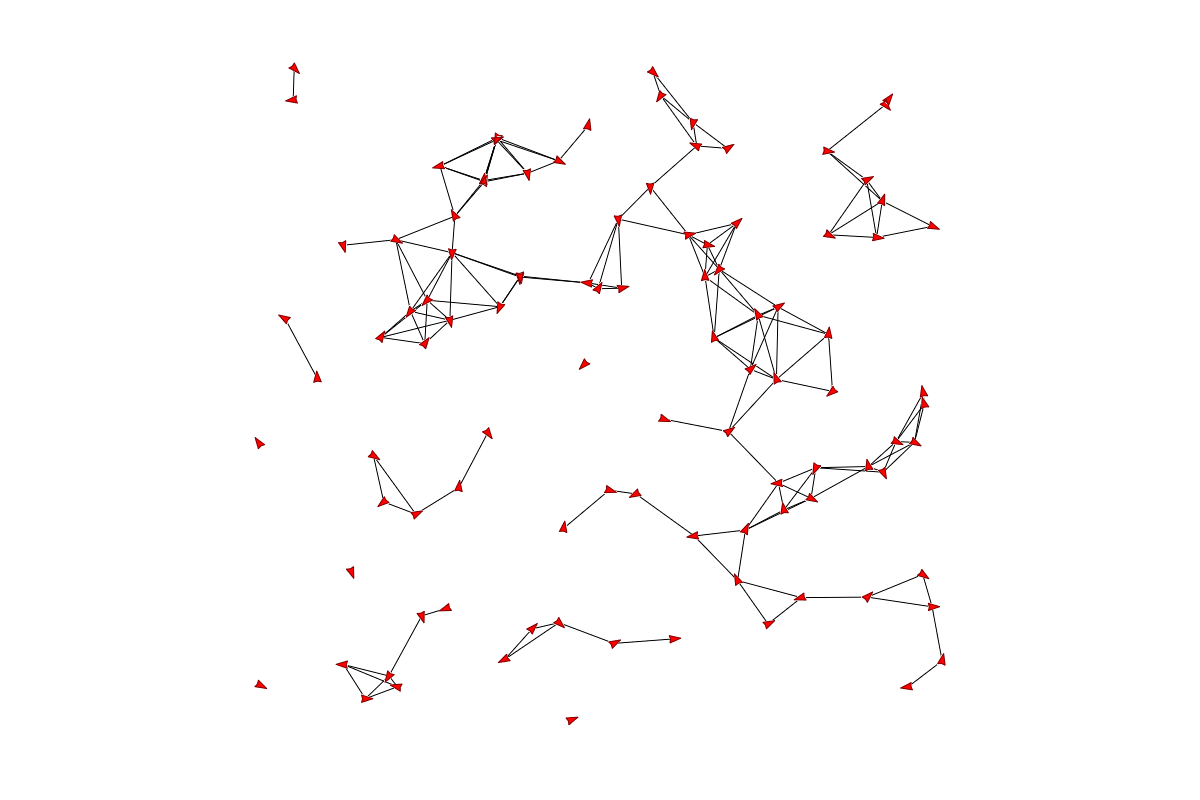
\includegraphics[trim=5cm 0cm 5cm 0cm, clip=true, width=0.8\textwidth]{figs/octsq100_init.png}
   \bigskip
   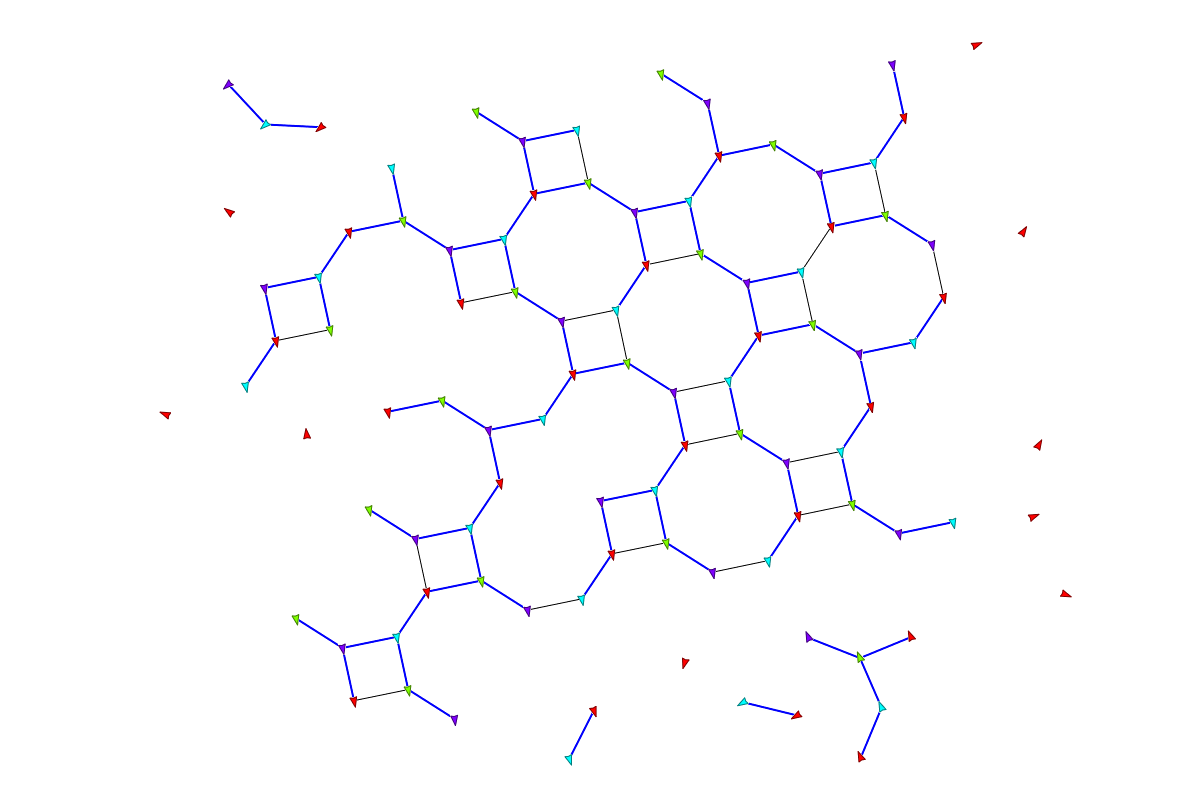
\includegraphics[trim=5cm 0cm 5cm 0cm, clip=true, width=0.8\textwidth]{figs/octsq100_final.png}
   \caption{[top] The initial poses of $100$ robots. [bottom] The final repeating hexagon pattern.}
   \label{fig:octagonsquare-init-final}
\end{figure}

%%%%%%%%%%%%%%%%%%%%%%%%%%%%%%%%%%%%%%%%
\begin{figure}
    \centering
  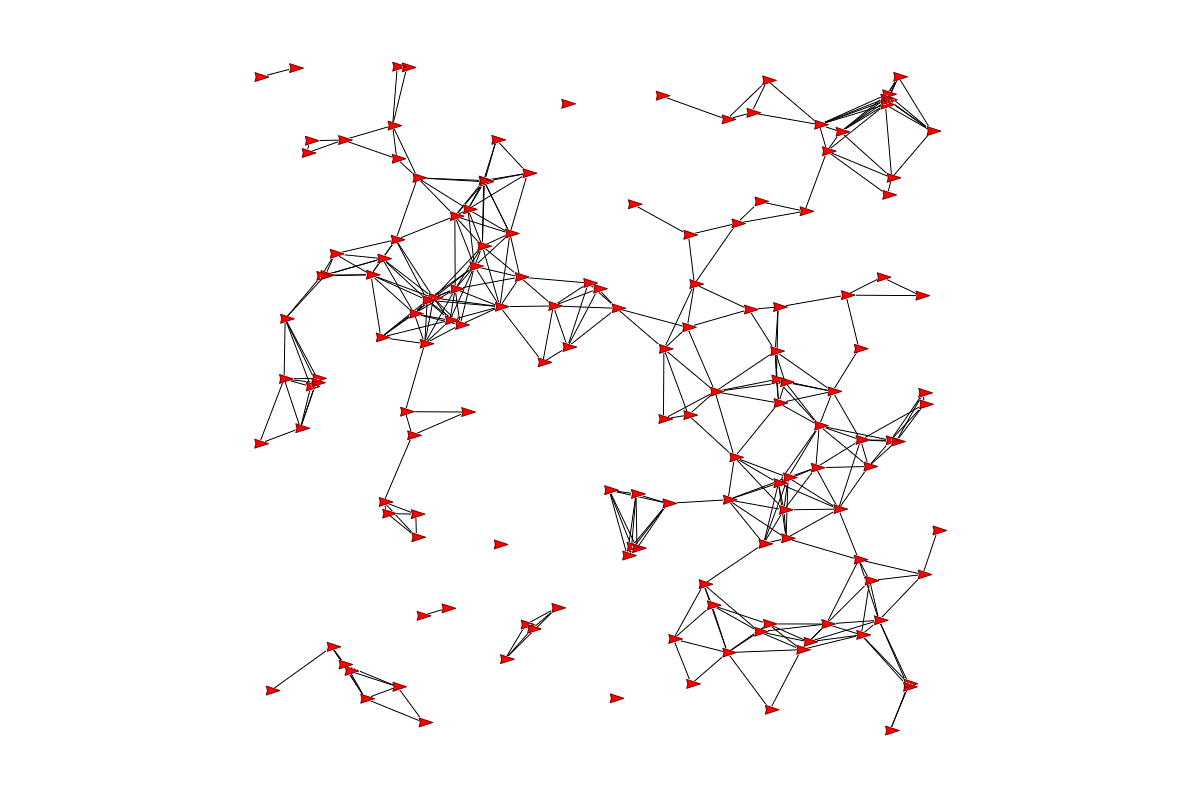
\includegraphics[trim=5cm 0cm 5cm 0cm, clip=true, width=0.8\textwidth]{figs/hex150_init.png}
  \bigskip
  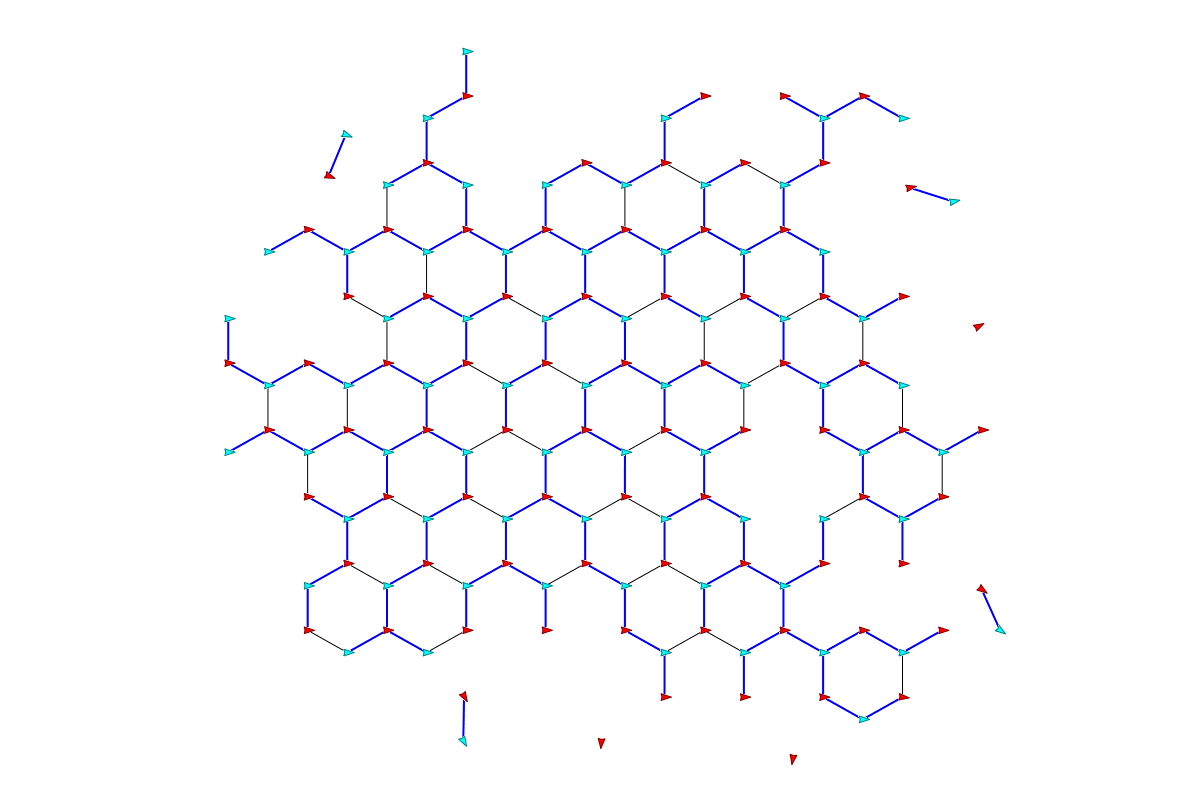
\includegraphics[trim=5cm 0cm 5cm 0cm, clip=true, width=0.8\textwidth]{figs/hex150_final.png}
  \caption{[top] The initial poses of $150$ robots. [bottom] The final repeating hexagon pattern.}
  \label{fig:hex-init-final}
\end{figure}


%%%%%%%%%%%%%%%%%%%%%%%%%%%%%%%%%%%%%%%%
\begin{figure}
    \centering
  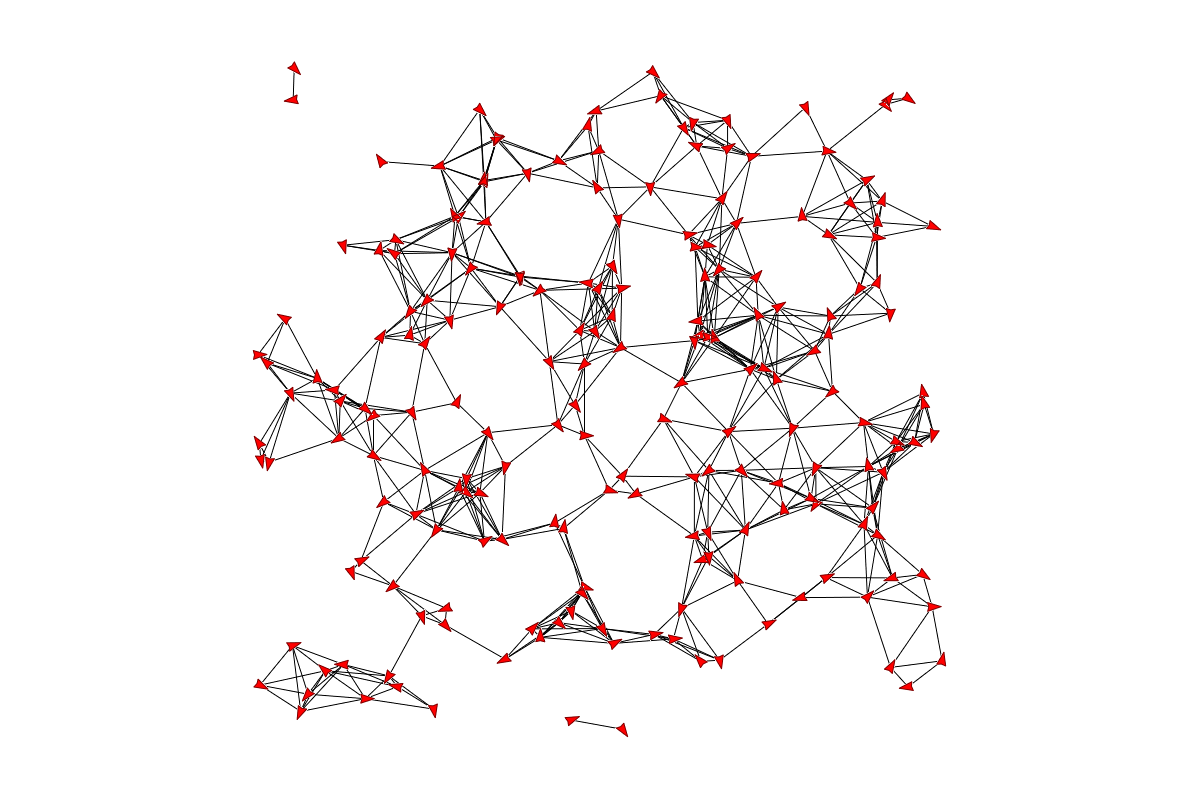
\includegraphics[trim=5cm 0cm 5cm 0cm, clip=true, width=0.8\textwidth]{figs/sq200_init.png}
  \bigskip
  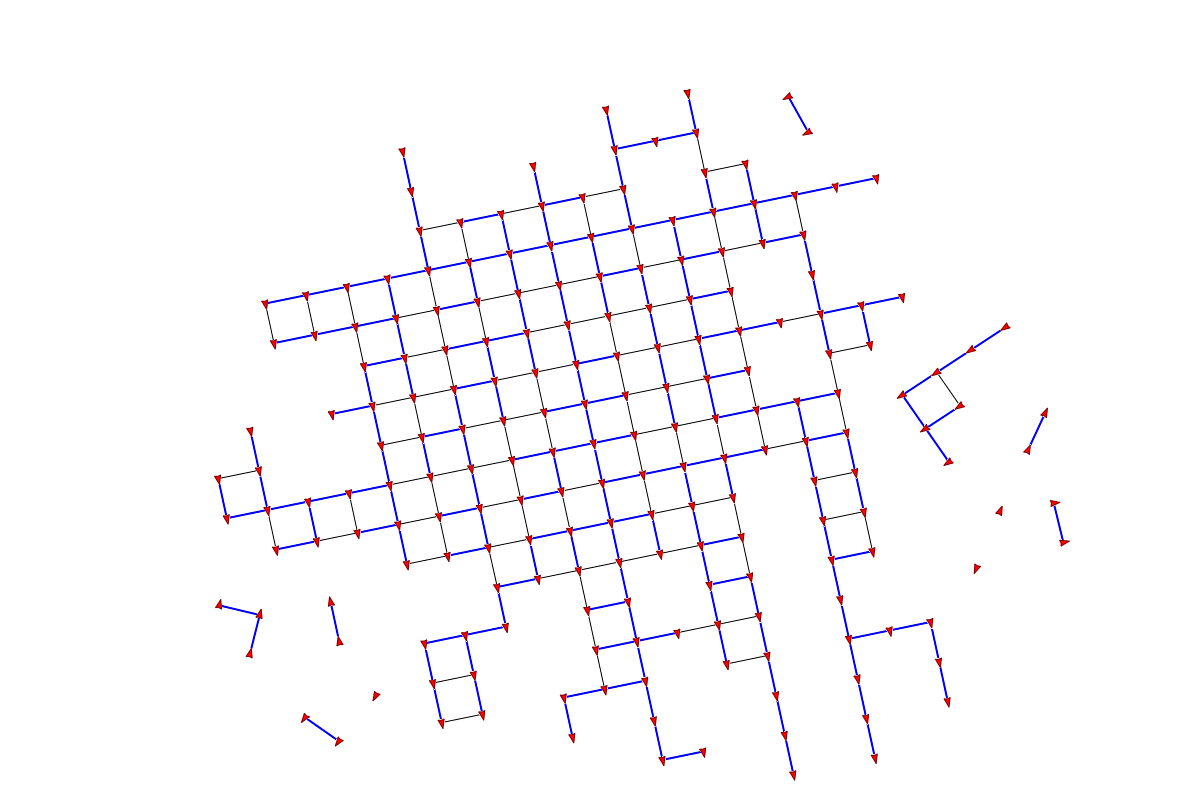
\includegraphics[trim=5cm 0cm 5cm 0cm, clip=true, width=0.8\textwidth]{figs/sq200_final.png}
  \caption{[top] The initial poses of $200$ robots. [bottom] The final repeating square pattern.}
  \label{fig:sq-init-final}
\end{figure}

We conclude from Figure~\ref{fig:exp-time} that the execution time scales reasonably with the increase of the number of robots, across all three given lattice graphs. 

%%%%%%%%%%%%%%%%%%%%%%%%%%%%%%%%%%%%%%%%
\begin{figure}
    \centering
   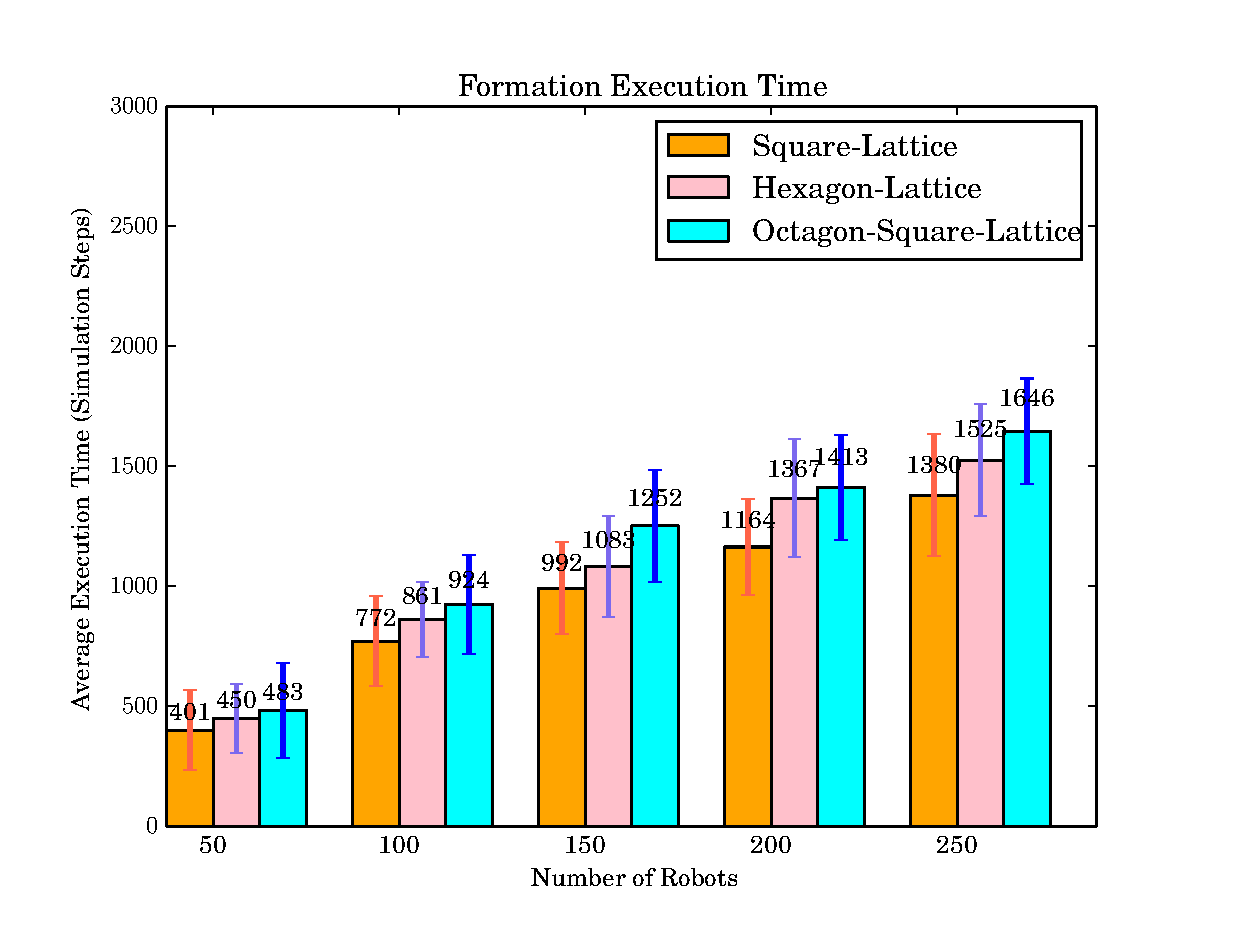
\includegraphics[width=\textwidth]{figs/exp_time}
    \caption{Average execution time and its standard deviation of forming repeated lattice patterns of square, hexagon and octagon-square.} 
    \label{fig:exp-time}
\end{figure}
%%%%%%%%%%%%%%%%%%%%%%%%%%%%%%%%%%%%%%%%

The initial distribution of robots' positions impacts the final formation quality in a certain sense.
%
Figure~\ref{fig:exp-qual} shows that when the number of robots is small and robots are sparsely distributed, most robots do not have enough neighbors around, thus the average formation fulfillment ratio is less than the result from a denser distribution. 
%
Moreover, Figure~\ref{fig:exp-qual} shows a trend that the fulfillment ratio for
a repeated pattern increases as the number of robots increases.

%%%%%%%%%%%%%%%%%%%%%%%%%%%%%%%%%%%%%%%%
\begin{figure}
    \centering
   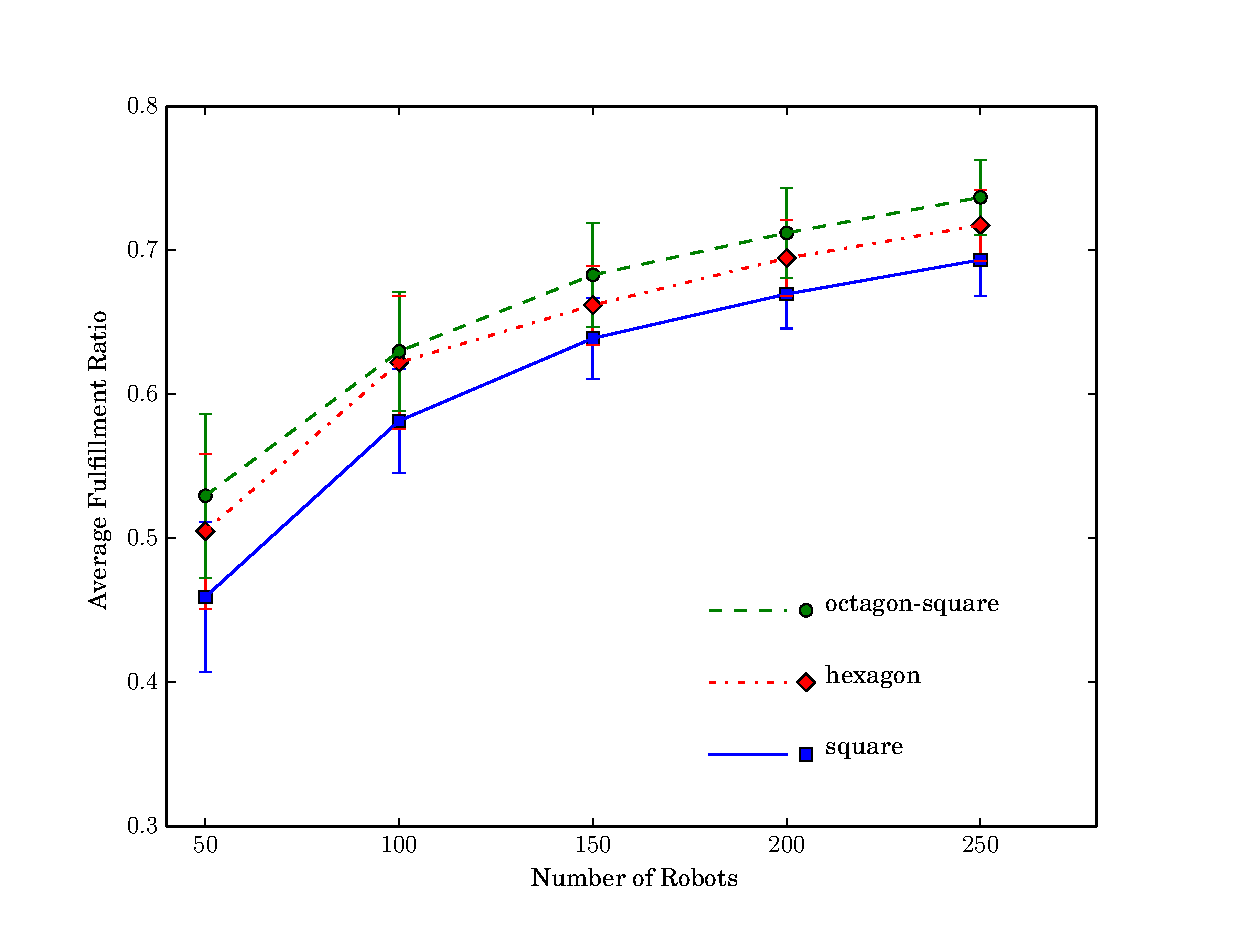
\includegraphics[width=\textwidth]{figs/exp_qual}
    \caption{Average fulfillment ratio and its standard deviation of forming lattice patterns of square, hexagon and octagon-square.} 
    \label{fig:exp-qual}
\end{figure}
%%%%%%%%%%%%%%%%%%%%%%%%%%%%%%%%%%%%%%%%


Additionally, we tested the robustness of our algorithm with another set of experiments.
%
Figure~\ref{fig:robust} shows one test case in which we removed some robots from the system when the system reached the static state for the first time.
%
Initially, $150$ robots formed a repeating hexagon pattern using the lattice graph (Figure~\ref{fig:hex}) as the input.  
%
It took $1441$ simulation steps for all robots to reach static states, with final fulfillment ratio $\Quality=0.804$. 
%
After randomly removed $50$ robots, it took another $1685$ simulation steps for robots to reach static states again, with the final fulfillment ratio $\Quality=0.713$. 
%
% Similar experiments were conducted and demonstrated that our algorithm works well after adding more robots to the system.

%%%%%%%%%%%%%%%%%%%%%%%%%%%%%%%%%%%%%%%%
\begin{figure}
    \begin{minipage}[b]{0.5\linewidth}
        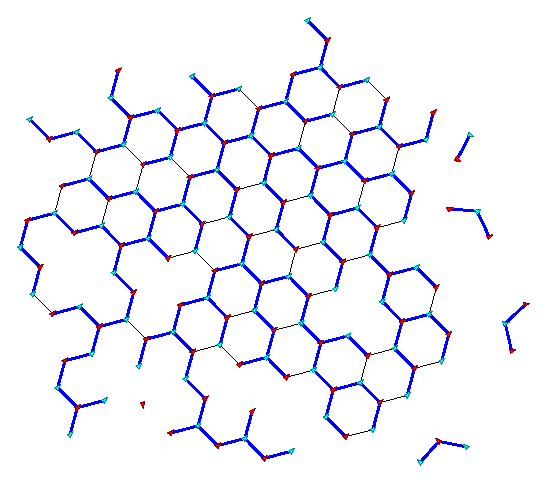
\includegraphics[width=.95\columnwidth]{figs/formation-150}
    \end{minipage}
    \begin{minipage}[b]{0.45\linewidth}
        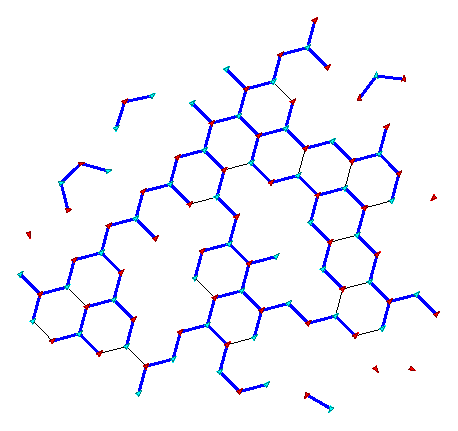
\includegraphics[width=.95\columnwidth]{figs/formation-100}
    \end{minipage}
    \caption{[left] The formation of repeated hexagon lattice with $150$ robots. [right] The reconfigured formation after randomly removed $50$ robots.}
\label{fig:robust}
\end{figure}
%%%%%%%%%%%%%%%%%%%%%%%%%%%%%%%%%%%%%%%%

Finally, we argue that our algorithm works well with non-repeating lattice patterns if we vary the problem assumptions.
%
In this case, a successful execution of our algorithm requires additional constraints: 
\begin{enumerate}
  \item The number of robots is the same as the number of vertices in the lattice graph.
  \item All robots are able to observe and communicate with each other initially.
\end{enumerate}
Because for a non-repeating lattice with finite number of vertices, 
we can simply use a lattice graph with the same number of nodes to represent the lattice.
%
For example, as shown in Figure~\ref{fig:p-letter}, a complete five-node lattice graph on the left represents the right ``P''-letter-like shape. 
%
It requires $n=5$ robots for a complete formation that satisfies the lattice graph with fulfillment ratio $1$.
If $n<5$, robots can never complete the desired shape. 
Otherwise, if there are more than $n>5$ robots, the $n-5$ robots must be either orphan robots or form another cluster of formations. 
Both cases do not satisfy the given lattice graph. 
% 
Without the second constraint, then the robots cannot distributed the tasks correctly to form the complete lattice.
\begin{figure}
    \centering
  \begin{minipage}[b]{0.45\linewidth}
  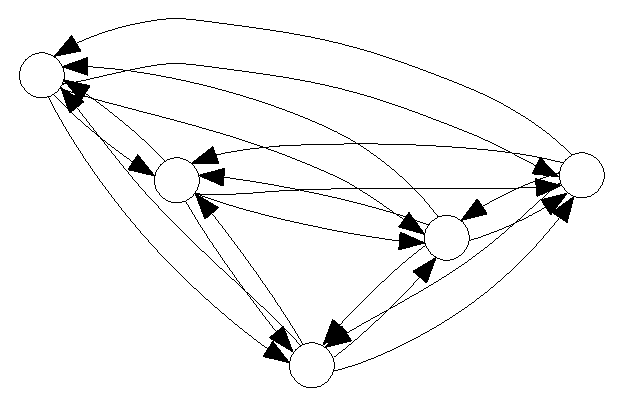
\includegraphics[width=.9\columnwidth]{figs/pletter}
  \end{minipage}
   \begin{minipage}[b]{0.45\linewidth}
     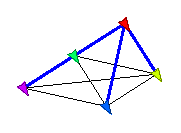
\includegraphics[width=.9\columnwidth]{figs/p-formation}
   \end{minipage}
   \caption{[left] A self-consistent lattice graph for letter ``P''. [right]
     Simulation result of the final formation. 
     The thick blue lines denote the edges in the authority tree.}
   \label{fig:p-letter}
 \end{figure}
 

%\clearpage
\section{Conclusions} 
\label{sec:conc-mrf1}
Above all, we conclude the strengths and weaknesses of our algorithm in this chapter.

First, the major advantages are listed as follows.
\begin{enumerate}
\item The algorithm enables multiple robots to form a broad diversity of lattice patterns autonomously with local information.
\item The algorithm runs efficiently and scales reasonably well with increasing numbers of robots.
\item The algorithm is robust to the situation when some robots fail to response others or when more robots join into the system.
\end{enumerate}


However, two limitations of this primary version are:
\begin{enumerate}
\item The algorithm cannot guarantee all the robots eventually reach static positions to form a global lattice pattern, since the lattice graph only reflects local relationships among robots' poses (Figure~\ref{fig:hex-qual}).
\item The motion strategy brings side effect on the final formation quality since the orphan robots, who are not assigned any destinations, might move to positions isolated from other robots.
\end{enumerate}

In the next chapter, we present another decentralized formation algorithm to solve these limitations, so that robots can form the desired global patterns in bounded time. 
Meanwhile, the lattice formation quality is improved.         %% The three sections of Chapter 1 
\chapter{Provably-Correct Formation Algorithm}
\label{chp:mrf2}
To resolve the limitations of our stateless formation algorithm proposed in Chapter~\ref{chp:mrf1}, we describe a new version of a stateful formation algorithm in this chapter.


The basic idea is to construct the desired lattice one element at a time. 
%
We recognize a robot's priority by identifying its ID's numerical order among the system, namely, the highest ID denotes the highest priority, the second highest ID denotes the second highest priority, and so on.
%
The robot with the highest ID acts as a ``root'' for the lattice.  
%
From there, the robot with the second highest ID moves to be a neighbor of the root robot,
assuming one of the neighbor positions defined by the lattice graph.
%
Meanwhile, other robots only move, if necessary, to maintain the connectivity
of communication graph.
%
By repeating this process, we sequentially drive one robot at a time to vacancies in the emerging formation, until all the robots are in place.
%
The primary challenges arise from the fact that each robot must execute this
strategy using only local information, and from the need to maintain
connectivity across all robots through the entire process.


The rest of this chapter is organized as follows. 
%
Section~\ref{sec:vacancy} introduces the concept of vacancy used in this algorithm. 
% 
Message passing plays an essential role for robots to interact and coordinate with each other.
%
In Section~\ref{sec:com}, we explain the communication protocols in the system.
%
That is, the procedure for each robot to generate its message periodically containing its some key global information retrieved from others' messages, such as the highest ID in the system.
%
During the algorithm execution, the robots will construct a spanning tree of the communication graph for the purpose of navigation.
%
%Section~\ref{sec:sptree} describe 
Therefore, the detail of constructing a spanning tree by each robot using only local communication is also discussed in this section.
%
Furthermore, we have designed a motion strategy to ensure the connectivity of the communication graph as long as the algorithm executes in Section~\ref{sec:mov}.
%
We have proved that our algorithm guarantees the robots to form the desired pattern in finite time in Section~\ref{sec:proof}.
%
Finally, in Section~\ref{sec:exp} we evaluate our algorithm by conducting groups of simulations and comparing the results with the results using the primary approach in Chapter~\ref{chp:mrf1}.


%\clearpage
\section{Vacancy}
\label{sec:vacancy}
One side effect of the stateless formation algorithm in Chapter~\ref{chp:mrf1} is the frequent formation ``destruction'' as the algorithm executes. 
%
Imagine that a cluster of robots reach positions and have formed 
a lattice.
If some other robots, whose authorities are higher than the authority of the cluster's root, are passing over. 
The existing lattice formation would be destroyed and the cluster of robots would re-organize themselves by constructing a new authority tree.


Figure~\ref{fig:destruction} shows an example, in which initially three robots $r_0, r_1, r_3$ form an authority tree, while robot $r_6$ forms another authority by itself.
%
After robots $r_0, r_1, r_3$ finish the local task assignment and reach positions, robot $r_1$ observes $r_6$.
%
Since robot $r_6$ owns the highest authority among all the robots, so these four robots reconstruct a new authority tree rooted at $r_6$. Then $r_6$ will assign tasks according to its neighbor and thus the formed lattice is destroyed.

%%%%%%%%%%%%%%%%%%%%%%%%%%%
\begin{figure}
\centering  
\begin{minipage}[b]{0.45\linewidth}
    \centering
    \begin{tikzpicture}[scale=1.5]
      \draw[fill=blue!50] (3,4.5) -- (2.75,5) -- (2.75,4.75) -- (2.5,4.75)   -- cycle;
      \node[color=blue] at (3.25, 5) {$r_0$};
      \draw[fill=blue!50] (5.2,3.92) -- (4.7,3.75) -- (5.2,3.58) -- (5.075,3.75)  -- cycle;
      \node[color=blue] at (5.4,3.75) {$r_1$};
      \draw[fill=red] (4,4) -- (3.75,4) -- (4.25,4.25) -- (4,3.75) -- cycle;
      \node[color=red] at (4, 3.5) {$r_3$};
      \draw[color=red] (3,4)  -- (3.125,4.17) -- (2.625,4) -- (3.125,3.83) -- cycle;
      \draw[dotted] (3,4) -- (4,4);
      \draw[color=red] (5,5) -- (4.75,5) -- (5.25,5.25) -- (5,4.75) -- cycle;
      \draw[dotted] (5,5) -- (4,4);
      \draw[dashed] (5,5) -- (5.075, 3.75);
      \draw[dashed] (3,4) -- (2.75,4.75);
      \draw[fill=orange] (6.2,5.5) -- (5.95,5.5) -- (6.45,5.75) -- (6.2,5.25)  -- cycle;
      \node[color=orange] at (6.7, 5.2) {$r_6$};
    \end{tikzpicture}
  \end{minipage}
  \begin{minipage}[b]{0.45\linewidth}
  \centering
    \begin{tikzpicture}[scale=1.5]
      \node[color=blue] at (3.25, 3.5) {$r_0$};
      \node[color=blue] at (5.1,4.5) {$r_1$};
      \draw[fill=blue!50] (4,4) -- (3.75,4) -- (4.25,4.25) -- (4,3.75) -- cycle;
      \node[color=blue] at (4, 3.5) {$r_3$};
      \draw[fill=blue!50] (3,4)  -- (3.125,4.17) -- (2.625,4) -- (3.125,3.83) -- cycle;
      \draw[] (3,4) -- (4,4);
      \draw[fill=blue!50] (5,5) -- (4.75,5) -- (5.25,5.25) -- (5,4.75) -- cycle;
      \draw[] (5,5) -- (4,4);
      \draw[fill=red] (6.2,5.5) -- (5.95,5.5) -- (6.45,5.75) -- (6.2,5.25)  -- cycle;
      \node[color=red] at (6.7, 5.2) {$r_6$};
      \draw[dotted] (5,5) -- (6.2,5.5);
    \end{tikzpicture}
  \end{minipage}
\caption{[left] The root robot $r_3$ assigns two positions to $r_1, r_0$, whereas robot $r_6$ is another root without any neighbor. [right] Robots $r_3, r_1, r_0$ reached assigned positions, and $r_1$ meets $r_6$ who owns the highest authority.}

\label{fig:destruction}
\end{figure}

Due to these unpredictable destruction phenomena, it is difficult for us to provide 
an upper bound of the algorithm execution time. 
%
In order to avoid this side effect, we want each robot to maintain a boolean state variable 
and track whether it is \textbf{stable} or \textbf{unstable}.  
%
The intuition is that stable robots remain motionless, whereas unstable robots
are either moving toward a vacancy or waiting for their turns do so.
%
Initially, each robot begins in the unstable state.
%
The unstable state changes permanently to the stable state when either the robot determines
that it has the highest ID over all robots (see Section~\ref{sec:com}), or the
robot finishes navigating to an open vacancy (see Section~\ref{sec:mov}).


The key idea of our algorithm is enabling the unstable robot with the highest ID to relocate itself 
to a position where it acts as a neighbor of the stable robot who owns the highest ID 
and does not yet have the maximum number of neighbors allowed by its role in the
lattice graph.

\begin{defn}
  For a stable robot $r_s$ with a role vertex $u$,
  there is a pose $\hat{p}$ corresponding to the vertex $w$
  corresponding each out-edge $e_{u}^w$ of $u$ in the lattice graph. 
  If there is no stable robot
  at $\hat{p}$, then $(\hat{p}, w)$ is a \textbf{vacancy} of $r_s$.
  (If, by chance, there is an \emph{unstable} robot at $\hat{p}$,
  we still consider $(\hat{p}, w)$ a vacancy of $r_s$.)
\end{defn}


Each stable robot periodically checks its surroundings for an open vacancy 
using Algorithm~\ref{alg:vacancy}. 

%%%%%%%%%%%%%%%%%%%%%%%%%%%%%%%%
\begin{algorithm}
%  \scriptsize
\SetKwInOut{Input}{input}
\SetKwInOut{Output}{output}
\SetKwData{OutEdge}{outEdge}
\SetKwData{Pose}{pose}
\SetKwData{NPose}{neighborPose}
\SetKwData{Obsv}{observations}
\SetKwArray{Vacancies}{vacancies}
\SetKwData{V}{Vacancy}
\SetKwData{InMsgs}{inMsgs}
\SetKwData{TNode}{terminalVertex}
\SetKwData{NID}{neighborID}
\SetKwData{Stable}{stable}
\SetKwData{MyV}{my vacancy}
\SetKwData{Empty}{empty}
\SetKwData{Null}{null}
\Input{\InMsgs, \Obsv}
\Output{\MyV}
  \Vacancies $\leftarrow \{\}$\; 
  \ForEach{\OutEdge}{
    \Pose $\leftarrow$ getPosFromTransformation(\OutEdge)\;
    insert \V(\Pose, \OutEdge.\TNode) to \Vacancies\;
  } 
  \ForEach{$\Pose \mbox{\textbf{ in }} \Vacancies$}{
    \ForEach{$\NPose \mbox{\textbf{ in }} \Obsv$}{
        \If{$\InMsgs[\NID].\Stable$ \mbox{\textbf{ and }} $\NPose = \Pose$}{
            remove \Pose from \Vacancies\;
        }
    }
  }
  \Return \Vacancies.\Empty $?$ \Null $: \Vacancies[0]$\;
  \caption{Compute a vacancy of a stable robot}
  \label{alg:vacancy}
\end{algorithm}


Consider the lattice graph for a repeating square pattern (Figure~\ref{fig:sq}).
Figure~\ref{fig:vacancy} shows an example in which robot $r_6$
is the stable robot with the highest ID and has three vacancies computed in terms of the
lattice graph in Figure~\ref{fig:sq}. 
%
The robot with the second highest ID $r_5$ is also stable and is already a neighbor of $r_6$.
%
The unstable robot with the highest ID is robot $r_4$, which is moving toward the vacancy ahead of $r_6$.  
%
Robot $r_4$
will change its state from unstable to stable after it reaches this pose.

%%%%%%%%%%%%%%%%%%%%%%%%%%%%%%%%
\begin{figure}
  \centering
   \begin{tikzpicture}[scale=1.5]
    %\useasboundingbox (1,0.5) rectangle (5.5,5);
    % center 2.875 2.75
    \coordinate (S) at (2.875, 2.75);
    \def\shifty{1}
    \def\ddy{2.5}
    \coordinate (A) at (1.5, 4.125);
    \coordinate (B) at (4,4.25-\shifty);
    \draw[fill=blue] (3,2.92) -- (2.5,2.75) -- (3,2.58) -- (2.875,2.75) -- cycle;
    \def\offset{0.5}
    \node[color=blue] at (2.875, 2.75-\offset) {$r_6$};
    % vacancies
    \def\dx{1.5}
    \def\dy{1.5}
    \draw[color=blue] (3+\dx,2.92) -- (2.5+\dx,2.75) -- (3+\dx,2.58) -- (2.875+\dx,2.75) -- cycle;
    \draw[color=blue] (3-\dx,2.92) -- (2.5-\dx,2.75) -- (3-\dx,2.58) -- (2.875-\dx,2.75) -- cycle;
    %%%%%%%
    \draw[fill=blue] (3,2.92+\dy) -- (2.5,2.75+\dy) -- (3,2.58+\dy) -- (2.875,2.75+\dy) -- cycle;
    \node[color=blue] at (3, 3.25+\offset) {$r_5$};
    %%%%%%%%
    \draw[color=blue] (3,2.92-\dy) -- (2.5,2.75-\dy) -- (3,2.58-\dy) -- (2.875,2.75-\dy) -- cycle;
    % another two robots
    \draw[fill=red!50] (1.5,4.5) -- (1.33,4) -- (1.5,4.125) -- (1.67,4) -- cycle; % center .5 4.125
    \node[color=blue] at (1.5, 3.25+\offset) {$r_1$};
    \def\shiftx{1.25}
    \draw[fill=red] (3+\shiftx,3.42) -- (2.5+\shiftx,3.25) -- (3+\shiftx,3.08) -- (2.875+\shiftx,3.25) -- cycle;          
    \node[color=blue] at (4, 4.75-\shifty) {$r_4$};
    \draw[] (S) -- (A);
    \draw[] (S) -- (B);
    \coordinate (V) at (2.875-\dx,2.75);
    \draw[dashed, ->] (B) -- (V);
    % two children of r_i
    \coordinate (C) at  (5, 3.25);
    %\draw[fill=orange] (5,3.5) -- (4.83,3) -- (5, 3.25) -- (5.17,3) -- cycle; % center .\5 3.625
    \node[color=blue] at (5, 3.75) {$r_2$};
    % center or r_c
    \def\xcc{5}
    \def\ycc{3.25}
    \def\hrlen{0.375}
    \def\ylen{0.17}
    \def\xlen{0.125}
    \coordinate (CC) at (\xcc, \ycc);
    % center of r_d
    \def\xdc{4.875}
    \def\ydc{2}
    \def\longlen{0.25}
    \coordinate (DC) at (\xdc, \ydc);
    \draw[] (B) -- (CC);
    \draw[] (B) -- (DC);
    \draw[] (CC) -- (DC);
    \coordinate (CA) at (\xcc-\hrlen, \ycc);
    \coordinate (CB) at (\xcc+\xlen, \ycc+\ylen);
    \coordinate (CD) at (\xcc+\xlen, \ycc-\ylen);
    \draw[fill=orange] (CA) -- (CB) -- (CC) -- (CD) -- cycle;
    \coordinate (D) at (5.375-\offset, 4.5-\ddy);

    \node[color=blue] at (5.125, 3.95-\ddy) {$r_3$};

  
    \coordinate (DA) at (\xdc-\longlen, \ydc+\longlen);
    \coordinate (DB) at (\xdc, \ydc-\longlen);
    \coordinate (DD) at (\xdc+\longlen, \ydc);
    \draw[fill=teal] (DA) -- (DB) -- (DC) -- (DD) -- cycle;
    
    \coordinate (R5) at (2.875, 2.75+\dy);
    \draw[] (S) -- (R5);
    \draw[] (R5) -- (A);
    \draw[] (R5) -- (B);
  \end{tikzpicture}
  \caption{Robot $r_6$ be a stable robot, it has three neighbors
    $r_1, r_5, r_4$ and three vacancies (hollow).  
    Robot $r_4$ is the relocate robot
    and its ultimate destination is the vacancy ahead of
    $r_6$. }
  
  \label{fig:vacancy}
\end{figure}
%%%%%%%%%%%%%%%%%%%%%%%%%%%%%%%%


%\clearpage
\section{Communication Procedure}
\label{sec:com}
We assume that the robots communicate by broadcasting messages to their
neighbors every $\dt$ seconds.
%
The main objective for the communication is to retrieve the principal global
information of the system and to construct a spanning tree of the
communication graph.


The principal global information includes: 
\begin{enumerate}
\item The \textbf{highest ID} among all robots in the network.
\item The \textbf{root robot}: the stable robot who has the highest ID and at least one vacancy. 
    It will be elected by others as the root of the spanning tree.
\item The \textbf{most important vacancy}: we order the vacancies of the root robot according to the numerical order of their corresponding vertices' IDs, then choose the first one as the most important vacancy.
%\item the highest ID among all unstable robot;
\item The \textbf{relocate robot}: the unstable robot who has the highest ID, it should relocate to the most important vacancy.
\end{enumerate}


We define a message type for robots to broadcast.
%
Table~\ref{tab:msg} lists the data contained in the message for robots to acquire the principal global information. 
%
The purpose of tracing the paths from the root and the relocate robots is
to prevent the ``rumors,'' in which a robot relies upon the
information generated originally by itself.  
%
Specifically, a robot
rejects information for which its own ID appears in the
``pathFromRoot'' or ``pathFromRelocate'' lists.
%
The memory consumption for the message passing process is upper bounded by a value linear to the number of the robots in the system. 

\begin{table}
\caption{Data included in each message.}
   \begin{tabular}{ll}
    \toprule
    \textbf{Data}  & \textbf{Description}  \\
    \midrule
    \textbf{senderID} &  ID of the robot that sent this message\\
    \midrule
    \textbf{highestID} & the highest robot ID in the system\\
    \midrule
    \textbf{rootID} &  ID of the root robot\\
    \midrule
    \textbf{relocateID} &  ID of the relocate robot\\
    \midrule
    \textbf{parentID} &  ID of the sender robot's spanning tree parent \\
    \midrule
    \textbf{vacancy} & the most important vacancy of the root robot\\
    \midrule
    \textbf{subtree} & a boolean marker showing if the sender robot is \\
        & in the subtree rooted at the relocate robot \\
    \midrule
    \textbf{stable} & a boolean label which indicates if the sender robot \\
        & is stable\\
    \midrule
    \textbf{pathFromRoot} & a list of robot IDs who are in the shortest\\
        & path to the root robot\\
    \midrule
    \textbf{pathFromRelocate} & a list of robot IDs who are in the shortest \\
        & path to the relocate robot\\
    \bottomrule
  \end{tabular}
  \label{tab:msg}
\end{table}

For all the robots to reach consensus about the principal global
information, 
we set up a time parameter, called ``communication timeout'', for robots to learn about the network enough. 
%
A proper value for the communication timeout is related with the
initial distribution of the robots' poses and the shape and dimensions of the
final formation. 
%
In the worst case, the communication timeout can be bounded
above by a time linear in the number of robots.


\begin{defn}
  \label{def:timeout}
  The \textbf{communication timeout} is the number of time steps that the robot
  needs to wait before it is confident about the principal information from the
  incoming messages.
\end{defn}


Our algorithm uses the communication timeout in two related ways (Algorithm~\ref{alg:timeout}).
%
First, each robot waits until the communication timeout has passed starting from the
last change to the highest ID that the robot knew about.  
%
When this occurs,
the robot can correctly decide whether it is or is not the highest ID robot.
%
The robot that does have the highest ID can then become stable.
%
Second, the robots use the communication timeout to identify
the unstable robot with the highest ID in the same way as identifying the highest ID.  
%
This robot then becomes the relocate
robot, and begins navigating toward the most important vacancy.

\begin{algorithm}
%  \scriptsize
\SetKwInOut{Input}{input}
\SetKwInOut{Output}{output}
\SetKwData{MyPreMsg}{myPreMsg}
\SetKwData{MyCurMsg}{myCurMsg}
\SetKwData{TIMEOUT}{TIMEOUT}
\SetKwData{HighestID}{highestID}
\SetKwData{RelocateID}{relocateID}
\SetKwData{CurrentTime}{currentTime}
\SetKwData{RootID}{rootID}
\SetKwData{MyID}{myID}
\SetKwData{V}{vacancy}
\SetKwData{Arr}{I am at the vacancy pose}
\SetKwData{LCH}{lastChangeToHighestID}
\SetKwData{LCR}{lastChangeToRelocateID}
\SetKwData{LCRt}{lastChangeToRootID}
\Input{\MyPreMsg, \MyCurMsg, \TIMEOUT}
\Output{void}
  \If{\MyPreMsg.\HighestID $\neq$ \MyCurMsg.\HighestID}{
     \LCH = \CurrentTime\;
  }
  \If{\MyPreMsg.\RelocateID $\neq$ \MyCurMsg.\RelocateID}{
     \LCR = \CurrentTime\;
  }
  \If{\MyPreMsg.\RootID$\neq$ \MyCurMsg.\RootID}{
     \LCRt = \CurrentTime\;
  }
  \If{\CurrentTime - \LCH $\geq$ \TIMEOUT}{
    \If{\MyID $=$\MyCurMsg.\HighestID}{
        I become stable with role $0$\;
    }
  }
  \If{\CurrentTime - \LCR $\geq$ \TIMEOUT}{
    \If{$\MyID = \MyCurMsg.\RelocateID \mbox{\textbf{ and }} \Arr $}{
        I become stable with the role of \MyCurMsg.\V\;
    }
  }
  \caption{Update robot's knowledge with communication timeout}
  \label{alg:timeout}
\end{algorithm}

% %\clearpage
% \section{Algorithm}
% \label{sec:sptree}

During the communication process, each robot computes its message
based on the incoming messages from its neighbors. 
%
Each robot can determine the highest ID by repeatedly comparing its own ID with the highest IDs transmitted by neighbors.
%
% The robots compute the highest ID unstable robot and the highest ID stable
% robot with vacancy in a similar way.

Moreover, in the same communication process, the robots construct a spanning
tree of their communication graph rooted at the highest ID stable robot with
vacancy.  
%
Each robot that has at least one stable neighbor, chooses the stable neighbor that has the fewest hops from the root as its parent in this tree.
%
Each robot without stable neighbors chooses the unstable neighbor with the minimal hops to the root as its parent.  
%
A special exception, designed to reduce unnecessary movements, is that no robot chooses the relocate robot as its parent, if it has another neighbor with the same or fewer hops to the root.  
%
Ties, if any, are broken in favor of the highest ID.  


Algorithm~\ref{alg:msg} briefly illustrates the communication process in which a robot reasons about the principle global information and its role in the spanning tree.
%
Specifically, Algorithm~\ref{alg:parent} describes the procedure for a robot to select a parent. 


Figure~\ref{fig:spanningtree} shows an example of a spanning tree of six robots.
%
Because the motion strategy uses the parent-child relationships in this
spanning tree to maintain connectivity, each robot also keeps track of whether
the relocate robot is its ancestor in the spanning tree, denoted ``subtree'' in
the message type.


\begin{algorithm}
    \SetKwInOut{Input}{input}
    \SetKwInOut{Output}{output}
    \SetKwData{InMsgs}{inMsgs}
    \SetKwData{MyMsg}{myMsg}
    \SetKwData{MyID}{myID}
    \SetKwData{HighestID}{highestID}
    \SetKwData{Stable}{stable}
    \SetKwData{RootID}{rootID}
    \SetKwData{Empty}{empty}
    \SetKwData{Null}{null}
    \SetKwData{SenderID}{senderID}
    \SetKwData{Obsv}{observations}
    \SetKwData{MyVacancy}{myVacancy}
    \SetKwData{Msg}{msg}
    \SetKwData{ParentID}{parentID}
    \SetKwData{ParentMsg}{parentMsg}
    \SetKwData{V}{vacancy}
    \SetKwData{Subtree}{subtree}
    \SetKwData{RelocateID}{relocateID}
    \SetKwData{EM}{eligibleMsgs}
    \SetKwData{PFR}{pathFromRelocate}
    \SetKwData{PFRt}{pathFromRoot}
    \SetKwData{MRtP}{minRootPath}
    \SetKwData{MRP}{minRelocatePath}
    \SetKwData{VFM}{vacancyFromMsgs}
    \SetKwFunction{FuncCV}{computeVacancy}
    \SetKwFunction{FuncGSPFRt}{getShortestPathFromRoot}
    \SetKwFunction{FuncGSPFR}{getShortestPathFromRelocate}
    \SetKwFunction{FuncGPM}{getParentMsg}
    \Input{\InMsgs}
    \Output{\MyMsg}
    \MyMsg.\SenderID $\leftarrow$ \MyID\;
    \MyMsg.\HighestID $\leftarrow$ \MyID\;
    \MyMsg.\Stable $\leftarrow$ \Stable\;
    \MyVacancy $\leftarrow$ \Stable $?$ \FuncCV(\InMsgs, \Obsv) $:$ \Null\;
    \MyMsg.\RootID $\leftarrow$ (\Stable \mbox{\textbf{ and }} \MyVacancy $\neq$ \Null) $?$ \MyID $ : -\infty$\;
    \MyMsg.\RelocateID $\leftarrow$ \Stable $ ? -\infty$ : \MyID\;
    \EM $\leftarrow$ \{\}\;
    \VFM $\leftarrow$ \Null\;
    \ForEach{\Msg \mbox{\textbf{ in }} \InMsgs}{
        \MyMsg.\HighestID $\leftarrow$ $\max$(\MyMsg.\HighestID, \Msg.\HighestID)\;
        \If{\mbox{\textbf{ not }} \Msg.\PFRt.contains(\MyID) \mbox{\textbf{ and }} \mbox{\textbf{ not }} \Msg.\PFR.contains(\MyID) }{
        insert \Msg into \EM\;
        \If{\Msg.\RootID $>$ \MyMsg.\RootID}{
            \MyMsg.\RootID $\leftarrow$ \Msg.\RootID\;
            \VFM $\leftarrow$ \Msg.\V\;
        }
        \MyMsg.\RelocateID $\leftarrow \max(\MyMsg.\RelocateID, \Msg.\RelocateID)$\;
        }
    }
    \MRtP $\leftarrow$ \FuncGSPFRt(\EM)\;
    \MRP $\leftarrow$ \FuncGSPFRt(\EM)\;
    \MyMsg.\V $\leftarrow$ (\MyID $=$ \MyMsg.\RootID) $?$ \MyVacancy $:$ \VFM\;
    \MyMsg.\PFRt $\leftarrow$ \MRtP.append(\MyID)\;
    \MyMsg.\PFR $\leftarrow$ \MRP.append(\MyID)\;
    \If{\MyID $\neq$ \MyMsg.\RootID}{
        \ParentMsg $\leftarrow$ \FuncGPM(\EM, \MyMsg, \RelocateID)\;
        \MyMsg.\ParentID $\leftarrow$ \ParentMsg.\SenderID\;
        \MyMsg.\Subtree $\leftarrow$ \MyID $=$ \MyMsg.\RelocateID \mbox{\textbf{ or }} \ParentMsg.\Subtree\;
    }
    \Return \MyMsg\;
    \caption{Compute message.}
    \label{alg:msg}
\end{algorithm}

%%%%%%%%%%%%%%%%%%%%%%%%%%%%%%%%
\begin{algorithm}
%  \scriptsize
\SetKwInOut{Input}{input}
\SetKwInOut{Output}{output}
  \SetKwData{InMsgs}{inMsgs}
    \SetKwData{MyMsg}{myMsg}
    \SetKwData{MyID}{myID}
    \SetKwData{HighestID}{highestID}
    \SetKwData{Stable}{stable}
    \SetKwData{RootID}{rootID}
    \SetKwData{Empty}{empty}
    \SetKwData{Null}{null}
    \SetKwData{SenderID}{senderID}
    \SetKwData{Obsv}{observations}
    \SetKwData{MyVacancy}{myVacancy}
    \SetKwData{Msg}{msg}
    \SetKwData{PID}{parentID}
    \SetKwData{PM}{parentMsg}
    \SetKwData{V}{vacancy}
    \SetKwData{Subtree}{subtree}
    \SetKwData{RelocateID}{relocateID}
    \SetKwData{EM}{eligibleMsgs}
    \SetKwData{PFR}{pathFromRelocate}
    \SetKwData{PFRt}{pathFromRoot}
    \SetKwData{MRtP}{minRootPath}
    \SetKwData{MRP}{minRelocatePath}
    \SetKwData{VFM}{vacancyFromMsgs}
    \SetKwData{MS}{mySteps}
    \SetKwData{MinSteps}{minSteps}
    \SetKwData{SM}{stableMsgs}
    \SetKwData{MWMS}{msgWithMinSteps}
    \SetKwData{UncleMsgs}{uncleMsgs}
    \SetKwData{Size}{size}
\Input{\EM, \MyMsg, \RelocateID}
\Output{\PM}
  %\PM $\leftarrow \{\}$\;
  \ForEach{\Msg \mbox{\textbf{ in }} \EM}{
    \If{\Msg.\Stable}{
      insert \Msg to \SM\;
    }
  }
  \If{\mbox{\textbf{ not }} \SM.\Empty}{
    \Return \MWMS \mbox{\textbf{ in }}  \SM\;
  }
  \MinSteps $\leftarrow$ \MyMsg.\PFRt.length\;
  \UncleMsgs $\leftarrow \{\}$\;
  \ForEach{\Msg \mbox{\textbf{ in }} \EM}{
    \MinSteps $\leftarrow \min$(\Msg.\PFRt.length, \MinSteps)\;
  }
  \ForEach{\Msg \mbox{\textbf{ in }} \EM}{
    \If{\Msg.\PFRt.length $=$ \MinSteps}{
        insert \Msg to \UncleMsgs\;
    }
  }
  sort \UncleMsgs in descending order of senderIDs\;
  \If{\MyID $\neq$ \RelocateID \mbox{\textbf{ and }} \mbox{\textbf{ not }} \UncleMsgs.\Empty}{
    \If{$\UncleMsgs[0].\SenderID = \RelocateID$}{
        \Return $\UncleMsgs.\Size > 1 ? \UncleMsgs[1] : \UncleMsgs[0]$\;
    }
  }  
  \Return $\UncleMsgs.\Empty ? \Null : \UncleMsgs[0]$\;
  \caption{Select the parent and return the parent's message.}
  \label{alg:parent}
\end{algorithm}

%%%%%%%%%%%%%%%%%%%%%%%%%%%%%%%%
\begin{figure}
   \centering
   \begin{minipage}[b]{0.45\linewidth}
  \centering
    \begin{tikzpicture}[scale=1.5]
      \draw [color=blue] (4,4) -- (3.2,3); % r1--r3
      \draw [color=blue] (4,4) -- (5.075,5.25); %r3--r5
      \draw [color=blue] (4,4) -- (2.75,4.75); % r3--r4
      \draw [color=blue] (4,4) -- (4.25, 3.25); %r3--r0
      \draw [color=blue] (2.75,4.75) -- (2.075,3.75); % r4--r2
      \draw [color=blue] (3.2,3) -- (2.075,3.75); % r1--r2
      \draw [color=blue] (3.2,3) -- (4.25,3.25); %r1--r0
      \draw[fill=red] (3,4.5) -- (2.75,5) -- (2.75,4.75) -- (2.5,4.75)   -- cycle;
      \node[color=blue] at (3.25, 5) {$r_4$};
      \draw[fill=blue] (5.2,5.42) -- (4.7,5.25) -- (5.2,5.08) -- (5.075,5.25)  -- cycle;
      \node[color=blue] at (5.2,4.75) {$r_5$};
      \draw[fill=green] (4,4) -- (3.75,4) -- (4.25,4.25) -- (4,3.75) -- cycle;
      \node[color=blue] at (4, 4.5) {$r_3$};
      \draw[fill=orange] (2.2,3.92) -- (1.7,3.75) -- (2.2,3.58) -- (2.075,3.75)  -- cycle;
      \node[color=blue] at (2, 3.25) {$r_2$};
      \draw[fill=cyan] (3.2,3) -- (2.95,3) -- (3.45,3.25) -- (3.2,2.75)  -- cycle;
      \node[color=blue] at (2.75, 2.8) {$r_1$};
      \draw[fill=purple] (4.5,3) -- (4.25,3.5) -- (4.25,3.25) -- (4,3.25)   -- cycle;
      \node[color=blue] at (4.25, 2.8) {$r_0$};    
    \end{tikzpicture}
  \end{minipage}
  \begin{minipage}[b]{0.45\linewidth}
    \centering
    \begin{tikzpicture}[scale=1.5]
      \tikzstyle{every state}=[fill=purple!50, draw=none]
      \node[state, scale=0.7] (A) at (2,3) {\large{$r_5$}};
      \node[state, scale=0.7] (B) at (2,2) {\large{$r_3$}};
      \node[state, scale=0.7] (C) at (2,1) {\large{$r_1$}};
      \node[state, scale=0.7] (D) at (1,1) {\large{$r_0$}};
      \node[state, scale=0.7, fill=orange!50] (E) at (3,1) {\large{$r_4$}};
      \node[state, scale=0.6, fill=orange!50] (F) at (4,0.5) {\large{$r_2$}};
      \draw[arc] (A) to[out=-90, in=90] (B);
      \draw[arc] (B) to[out=-90, in=90] (C);
      \draw[arc] (B) to[out=-135, in=45] (D);
      \draw[arc] (B) to[out=-45, in=135] (E);
      \draw[arc] (E) to[out=-25, in=150] (F);
    \end{tikzpicture}
  \end{minipage}
\caption{[left] Communication graph of six robots. [right] Assume
  $r_5$ has the highest stable ID and a vacancy. A spanning tree
  corresponding to the left communication graph is built, in which the
  root is $r_5$. Let $r_4$ be the relocate robot, it then is the root
  of the moving subtree, in which $r_2$ is its descendant.}

   \label{fig:spanningtree}
\end{figure}
%%%%%%%%%%%%%%%%%%%%%%%%%%%%%%%

%\clearpage
\section{Movement Strategy}
\label{sec:mov}

Similar to the previous method in Chapter~\ref{chp:mrf1}, we use the bounded movement idea from Lemma~\ref{lem:boundedrange} to maintain
the connection between two robots if there exists a parent-child relationship
between them in the tree structure.  
%
The intuition is, only the relocate robot and its descendants (if any) move, while ensuring no one falls disconnected with others in the system.
%
A key difference from the prior algorithm is an inversion of responsibility:
rather than tasking each robot in this subtree to remain within range of its
parent, we instead require each parent to obey a ``No Child Left Behind
(NCLB)'' policy, which allows only movements that are guaranteed to stay within
bounded range of each of its children.
%
In turn, each child moves close enough to its parent to enable the parent to
make progress in spite of the NCLB constraint.
%
Specifically, each moving robot computes in the intersection of the bounded
ranges of its children.  
%
This intersection region forms a ``safe region'' such
that if the robot stays with its safe region, it can guarantee to remain within
range of all of its children in the next time step.  
%
A robot that stays within
its safe region is said to obey NCLB.


Recall the scenario in Figure~\ref{fig:vacancy}.
Robot $r_4$ is moving towards to the vacancy ahead of robot $r_6$. 
%
With the NCLB policy, robot $r_4$ computes an intermediate goal $g_4$ within the safe region of $r_2, r_3$ (shaded region), since it is an ancestor of the two robots, as shown in Figure~\ref{fig:nclb}.

The movement strategy falls into three cases.
\begin{enumerate}
  \item If a robot is stable, or it is not in the moving subtree, then it does
  not move.

  \item If a robot is the relocate robot, it moves
  toward its parent, unless its parent is the root, in which case it moves
  toward the vacancy, without violating NCLB.
  % 
  Figure~\ref{fig:nclb} shows a scenario in which a relocate robot
  computes an intermediate goal according to the bounded ranges of its
  children.

  \item For other robots in the moving subtree, we set a ``safe distance'',
  denoted $d_s = \range-v\dt$.  If the robot is within distance $d_s$ of
  its parent, it does not move.  Otherwise, moves it directly toward its parent
  while staying within its NCLB safe region.
  %
\end{enumerate}

A special case occurs if the safe region for any robot is empty.
%
In that case, the robot does not move.  
%
We can still guarantee connectivity in this case
because the children (which must exist to get an empty safe region) will only
move toward the robot.  
%
Movements that decrease the distance between robots
cannot break their connectivity.  
%
If \hbox{$d_s < \range - v\dt$}, then the safe
region will eventually be non-empty (Figure~\ref{fig:safedist2}).

Figure~\ref{fig:safedist} gives another example of the NCLB movement strategy,
in which the relocate robot $r_4$ first waits for its child $r_2$ to come closer, then
computes its intermediate goal $g_4$ in the bounded range $B_2$ of its children.


In this way, the relocate robot navigates to the vacancy by tracing its path to the root.  
%
It then changes its
state from unstable to stable, triggering the communication process to identify
the next relocate robot and the next vacancy.  
%
After each robot moved to a vacancy, the formation is complete, and the algorithm terminates upon
discovering that no unstable robots remain.

%%%%%%%%%%%%%%%%%%%%%%%%%%%%%%%%
\begin{figure}
\centering
\begin{tikzpicture}[scale=1.25]
    \tikzstyle{ann} = [fill=white, font=\footnotesize,inner sep=1pt]   
    %\useasboundingbox (1,0.5) rectangle (5.5,5);
    % center 2.875 2.75
    \def\xs{2.875}
    \def\ys{2.75}
    \coordinate (S) at (\xs, \ys);
    \def\shiftx{1.25}               
    \def\shifty{1}
    \def\ddy{2.5}
    \def\offset{0.5}
    \def\movedist{1.65}
    \coordinate (A) at (1.5, 4.125);
    \coordinate (B) at (4,4.25-\shifty); % r_i
    \def\xrc{5}
    \def\yrc{3.25}
    \coordinate (C) at (\xrc, \yrc);
    \def\xrd{4.875}
    \def\yrd{2}
    \coordinate (D) at (\xrd, \yrd);
     % ranges of r_c and r_d
    \def\childcircleD{(D) circle (\movedist)}
    \def\childcircleC{(C) circle (\movedist)}
    \draw[orange] \childcircleC;
    \draw[teal] \childcircleD;
    % intersection region of children's ranges
    \begin{scope}
      \clip \childcircleC;
      \filldraw[fill=yellow!20] \childcircleD;
    \end{scope}
    
    \draw[fill=blue] (3,2.92) -- (2.5,2.75) -- (3,2.58) -- (2.875,2.75) -- cycle;
    \node[color=blue] at (2.875, 2.75-\offset) {$r_6$};
    \draw[fill=red!50] (1.5,4.5) -- (1.33,4) -- (1.5,4.125) -- (1.67,4) -- cycle; % center .5 4.125
    % vacancies
    \def\dx{1.5}
    \def\dy{1.5}
    \draw[color=blue] (3+\dx,2.92) -- (2.5+\dx,2.75) -- (3+\dx,2.58) -- (2.875+\dx,2.75) -- cycle;
    \draw[color=blue] (3-\dx,2.92) -- (2.5-\dx,2.75) -- (3-\dx,2.58) -- (2.875-\dx,2.75) -- cycle;
   % \draw[color=blue] (3,2.92+\dy) -- (2.5,2.75+\dy) -- (3,2.58+\dy) -- (2.875,2.75+\dy) -- cycle;
    %%%%%%%
    \draw[fill=blue] (3,2.92+\dy) -- (2.5,2.75+\dy) -- (3,2.58+\dy) -- (2.875,2.75+\dy) -- cycle;
    \node[color=blue] at (3, 3.25+\offset) {$r_5$};
    %%%%%%%%
    \draw[color=blue] (3,2.92-\dy) -- (2.5,2.75-\dy) -- (3,2.58-\dy) -- (2.875,2.75-\dy) -- cycle;
   
    \node[color=blue] at (1.25, 3.25+\offset) {$r_1$};
    %%%%%%%%%%%%%%%% triangle facing -135 degree
    \def\xc{4}
    \def\yc{3.25}
    \coordinate (TC) at (\xc, \yc);
    \def\longlen{0.25}
    \coordinate (TA) at (\xc-\longlen, \yc-\longlen);
    \coordinate (TB) at (\xc, \yc+\longlen);
    \coordinate (TD) at (\xc+\longlen, \yc);
 
    %%%%%%%%%%%%%%%%%%%%%%%%%%%%%%%%%%%%%%%%%%%%%
    \node[color=blue] at (3.9, 4.75-\shifty) {$r_4$};
    \draw[] (S) -- (A);
    \draw[] (S) -- (B);
  
    \node[color=blue] at (5.4, 3.25) {$r_2$};
    \draw[] (B) -- (C);
   
    \node[color=blue] at (5.4, 4.35-\ddy) {$r_3$};
    \draw[] (B) -- (D);
    \draw[] (C) -- (D);
    \coordinate (G) at (1.9+\dx,2.75);
    \draw[dotted] (2.875-\dx,2.75) -- (G);
    \draw[dashed] (B) -- (G);
    \def\goalcircleG{(G) circle (0.1)}
    \draw[fill=red] \goalcircleG;
    \node[ann] at (3.5,2.25) {$g_4$};
    % three robots
    \draw[fill=red] (TA) -- (TB) -- (TC) -- (TD) -- cycle;
    % draw r_c
    \def\xcc{5}
    \def\ycc{3.25}
    \def\hrlen{0.375}
    \def\ylen{0.17}
    \def\xlen{0.125}
    \coordinate (CC) at (\xcc, \ycc);
    \coordinate (CA) at (\xcc-\hrlen, \ycc);
    \coordinate (CB) at (\xcc+\xlen, \ycc+\ylen);
    \coordinate (CD) at (\xcc+\xlen, \ycc-\ylen);
    \draw[fill=orange] (CA) -- (CB) -- (CC) -- (CD) -- cycle;
    %\def\parentCircle {(S) circle (\movedist)}
    %\draw[color=blue] \parentCircle;
    % draw r_d  heading 135 degrees
    \def\xdc{4.875}
    \def\ydc{2}
    \coordinate (DC) at (\xdc, \ydc);
    \coordinate (DA) at (\xdc-\longlen, \ydc+\longlen);
    \coordinate (DB) at (\xdc, \ydc-\longlen);
    \coordinate (DD) at (\xdc+\longlen, \ydc);
    \draw[fill=teal] (DA) -- (DB) -- (DC) -- (DD) -- cycle;
    %%%%%%%%%%%%%% add texts of bounded ranges
    %\node[color=blue] at (\xs-0.75, \ys-\shifty) {$\B_s$};
    \node[color=orange] at (\xrc, \yrc+\shifty) {$\B_2$};    
    \node[color=teal] at (\xrd, \yrd-\shifty) {$\B_3$};
    
    \coordinate (R5) at (2.875, 2.75+\dy);
    \draw[] (S) -- (R5);
    \draw[] (R5) -- (A);
    \draw[] (R5) -- (B);
  \end{tikzpicture}
  \caption{The relocate robot $r_4$ has two descendants $r_2,
    r_3$ in the moving subtree. Two circles denote the bounded
    ranges of $r_2, r_3$, $r_4$ finds an intermediate goal (red dot)
    $g_4\in\left(\B_3 \cap \B_3\right)$.}
\label{fig:nclb}
\end{figure}
%%%%%%%%%%%%%%%%%%%%%%%%%%%%%%%%
\begin{figure}
\centering
\begin{minipage}{0.9\linewidth}
  \centering
  \begin{tikzpicture}[scale=1.1]
    \tikzstyle{ann} = [fill=white,font=\footnotesize,inner sep=1pt]
    % \useasboundingbox (1,0.5) rectangle (5.5,5);
    % center 2.875 2.75
    \coordinate (S) at (2.875, 2.75);
    \def\offset{0.5}
    \draw[fill=orange] (2.75,2.92) -- (3.25,2.75) -- (2.75,2.58) -- (2.875,2.75) -- cycle;
    \node[color=blue] at (2.875, 2.75-\offset) {$r_3$};
    \node[color=orange] at (3,3.75) {$\B_3$}; 
    % vacancy
    \def\dx{1.5}
    \def\ddx{2}
    \def\dddx{4.5}
    \coordinate (I) at (2.875+\ddx,2.75);
    \coordinate (C) at (2.875+\dddx,2.75);
    % \draw[color=blue] (3-\dx,2.92) -- (2.5-\dx,2.75) -- (3-\dx,2.58) -- (2.875-\dx,2.75) -- cycle;
    %\draw[fill=red] (3+\ddx,2.92) -- (2.5+\ddx,2.75) -- (3+\ddx,2.58) -- (2.875+\ddx,2.75) -- cycle;
    \draw[fill=red] (4.875, 3.125) -- (4.705,2.625) -- (4.875, 2.75) -- (5.045,2.625) -- cycle; 
    \node[color=blue] at (4.875+\offset, 2.75-\offset) {$r_4$};
    \draw[fill=teal] (3+\dddx,2.92) -- (2.5+\dddx,2.75) -- (3+\dddx,2.58) -- (2.875+\dddx,2.75) -- cycle;
    \node[color=blue] at (7.375, 2.75-\offset) {$r_2$};
    \draw[dotted] (I) -- (S);
    \draw[dotted] (I) -- (C);

    \def\rd{4}
    \coordinate (R3) at (4.875, 4.25);
    %\draw[fill=orange] (1.5,4.5) -- (1.33,4) -- (1.5,4.125) -- (1.67,4) -- cycle; % center .5 4.125
    \draw[fill=blue] (4.875, 0.625+\rd) -- (4.705,0.125+\rd) -- (R3) -- (5.045,0.125+\rd) -- cycle; 
    \node[color=blue] at (4.875+\offset, 4.25) {$r_6$};
    
    \draw[color=blue] (4.875, 5.625) -- (4.705,5.125) -- (4.875,5.25) -- (5.045,5.125) -- cycle; 
    \draw[dotted] (I) -- (4.875,5.25);

    \def\safedist{1.2}
    \def\circleSafeI {(I) circle (\safedist)}
    %\draw[color=red] \circleSafeI;
    \def\movedist{1.7}
    \def\circleMoveC {(C) circle (\movedist)}
    \def\circleMoveS {(S) circle (\movedist)}
    \draw[color=teal] \circleMoveC;
    \draw[color=orange] \circleMoveS;
    % radius of circleMoveC
    \draw[dashed,line width=.5pt] (7.375, 2.75-\movedist) -- (7.375+\movedist,2.75-\movedist);
    \draw[dashed,line width=.5pt] (7.375+\movedist, 2.75) -- (7.375, 2.75);
    \draw[arrows=<->,line width=.5pt] (7.375+\movedist,2.75-\movedist) -- (7.375+\movedist,2.75);
    \node[ann] at (9,2) {$\range-v\dt$};
    \coordinate (Cu) at (7.375, 3+\movedist);
    \coordinate (Iu) at (4.875, 3+\movedist);
    \draw[dashed, line width=.5pt] (C) -- (Cu);
    \draw[dashed, line width=.5pt] (I) -- (Iu);
    \draw[arrows=<->, line width=.5pt] (Cu) -- (Iu);
    \node[ann] at (6, 3+\movedist) {$\range$};
    \coordinate (Id) at (4.875, 2.5-\movedist);
    \coordinate (M) at (4.875+\safedist, 2.75);
    \coordinate (Md) at (4.875+\safedist, 2.5-\movedist);
    \draw[dashed, line width=.5pt] (I) -- (Id);
    \draw[dashed, line width=.5pt] (M) -- (Md);
    \coordinate (Id2) at (4.875, 2.75-\movedist);
    \coordinate (Md2) at (4.875+\safedist, 2.75-\movedist);
    \draw[arrows=<->, line width=.5pt] (Id2) -- (Md2);
    \node[ann] at (5.5, 2.75-\movedist) {$d_s$};
    %%%%
    % \def\parentCircle {(S) circle (\movedist)}
    % \draw[color=blue] \parentCircle;
    % \node[color=blue] at (3,3.75) {$\B_s$};
    \node[color=teal] at (8,3.75) {$\B_2$}; 
        %%%%           
    %% \coordinate (X) at (3.5-\dx, 2.75);
    %% \coordinate (Xd) at (3.5-\dx,2.75-\movedist);
    %% \draw[arrows=<->, line width=.5pt] (X) -- (Xd);
    %% \node[ann] at (1.75,2) {$\range-v\dt$};
    %% \coordinate (Sd) at (2.875, 2.75-\movedist);
    %% \draw[dashed,line width=.5pt] (Xd) -- (Sd);
    %% \draw[dashed,line width=.5pt] (S) -- (X);
  \end{tikzpicture}
\end{minipage}
\begin{minipage}{0.9\linewidth}
  \centering
   \begin{tikzpicture}[scale=1.1]
    \tikzstyle{ann} = [fill=white,font=\footnotesize,inner sep=1pt]
    % \useasboundingbox (1,0.5) rectangle (5.5,5);
    % center 2.875 2.75
    \coordinate (S) at (2.875, 2.75);
    \def\offset{0.5}
    \draw[fill=orange] (2.75+\offset,2.92) -- (3.25+\offset,2.75) -- (2.75+\offset,2.58) -- (2.875+\offset,2.75) -- cycle;
    \node[color=blue] at (2.875+\offset, 2.75-\offset) {$r_3$};
    \node[color=orange] at (3,3.75) {$\B_3$}; 
    \coordinate (D) at (2.875+\offset, 2.75);
    
    % vacancy
    \def\dx{1.5}
    \def\ddx{2}
    \def\dddx{3}
    \coordinate (I) at (2.875+\ddx,2.75);  %4.375, 2.75
    \coordinate (C) at (2.875+\dddx,2.75); %5.875, 2.75
    \def\safedist{1.2}
    \def\circleSafeI {(I) circle (\safedist)}
    %\draw[color=red] \circleSafeI;
    \def\movedist{1.7}
    \def\circleMoveC {(C) circle (\movedist)}
    \draw[color=teal] \circleMoveC;
    \def\circleMoveD {(D) circle (\movedist)}
    \draw[color=orange] \circleMoveD;
    \begin{scope}
      \clip \circleMoveC;
      \filldraw[fill=yellow!20] \circleMoveD;
    \end{scope}
    %\draw[color=blue] (3-\dx,2.92) -- (2.5-\dx,2.75) -- (3-\dx,2.58) -- (2.875-\dx,2.75) -- cycle;
    %\draw[fill=red] (3+\ddx,2.92) -- (2.5+\ddx,2.75) -- (3+\ddx,2.58) -- (2.875+\ddx,2.75) -- cycle;
    \draw[fill=red] (4.875, 3.125) -- (4.705,2.625) -- (4.875, 2.75) -- (5.045,2.625) -- cycle; 
    \node[color=blue] at (4.875+\offset, 2.75-\offset) {$r_4$};
    \draw[fill=teal] (3+\dddx,2.92) -- (2.5+\dddx,2.75) -- (3+\dddx,2.58) -- (2.875+\dddx,2.75) -- cycle;
    \node[color=blue] at (5.875+\offset, 2.75-\offset) {$r_2$};
    \draw[dotted] (I) -- (S);
    \draw[dotted] (I) -- (C);

    %%%%%%%%%%%%%%%%
    \coordinate (Cu) at (7.375, 3+\movedist);
    \coordinate (Iu) at (4.875, 3+\movedist);
    \coordinate (Co) at (7.375, 2.75);
    \draw[dashed, line width=.5pt] (Co) -- (Cu);
    \draw[dashed, line width=.5pt] (I) -- (Iu);
    \draw[arrows=<->, line width=.5pt] (Cu) -- (Iu);
    \node[ann] at (6, 3+\movedist) {$\range$};
    \coordinate (Id) at (4.875, 2.5-\movedist);
    \coordinate (M) at (4.875+\safedist, 2.75);
    \coordinate (Md) at (4.875+\safedist, 2.5-\movedist);
    \draw[dashed, line width=.5pt] (I) -- (Id);
    \draw[dashed, line width=.5pt] (M) -- (Md);
    \coordinate (Id2) at (4.875, 2.75-\movedist);
    \coordinate (Md2) at (4.875+\safedist, 2.75-\movedist);
    \draw[arrows=<->, line width=.5pt] (Id2) -- (Md2);
    \node[ann] at (5.5, 2.75-\movedist) {$d_s$};
    %%%%%%%%%%%%%%%%%
    \coordinate (N) at (5.875+\movedist, 2.75);
    \coordinate (Nd) at (5.875+\movedist, 2.75-\movedist);
    \draw[dashed,line width=.5pt] (N) -- (C);
    \draw[dashed,line width=.5pt] (Md2) -- (Nd);
    % radius of circleMoveC
    \draw[arrows=<->,line width=.5pt] (N) -- (Nd);
    \node[ann] at (8,2) {$\range-v\dt$};
    %%%% G.x = c.x - \movedist
    \coordinate (G) at (4.625, 3.9);
    \draw[fill=red] (G) circle (0.1);
    \node[ann] at (4.625, 3.9-\offset) {$g_4$};
    %%%%
    % \def\parentCircle {(S) circle (\movedist)}
    % \draw[color=blue] \parentCircle;
    %%%%
    %\node[color=blue] at (3,3.75) {$\B_s$};
    \node[color=teal] at (6,3.75) {$\B_2$}; 
    %% \coordinate (X) at (3.5-\dx, 2.75);
    %% \coordinate (Xd) at (3.5-\dx,2.75-\movedist);
    %% \draw[arrows=<->, line width=.5pt] (X) -- (Xd);
    %% \node[ann] at (1.75,2) {$\range-v\dt$};
    %% \coordinate (Sd) at (2.875, 2.75-\movedist);
    %% \draw[dashed,line width=.5pt] (Xd) -- (Sd);
    %% \draw[dashed,line width=.5pt] (S) -- (X);
    \def\rd{4}
    \coordinate (R3) at (4.875, 4.25);
    %\draw[fill=orange] (1.5,4.5) -- (1.33,4) -- (1.5,4.125) -- (1.67,4) -- cycle; % center .5 4.125
    \draw[fill=blue] (4.875, 0.625+\rd) -- (4.705,0.125+\rd) -- (R3) -- (5.045,0.125+\rd) -- cycle; 
    \node[color=blue] at (4.875+\offset, 4.25) {$r_6$};
    
    \draw[color=blue] (4.875, 5.625) -- (4.705,5.125) -- (4.875,5.25) -- (5.045,5.125) -- cycle; 
    \draw[dotted] (I) -- (4.875,5.25);
    
    \end{tikzpicture}
\end{minipage}
   \caption{(top) The relocate robot $r_4$ intends to move to the
   vacancy (hollow arrow) of the root robot $r_6$. Robots $r_2, r_3$ are 
   children of $r_4$. Since $\B_2\cap\B_2=\emptyset$, $r_4$
   waits for $r_2, r_3$ to move close to it. (bottom) When
   the safe region for $r_4$ becomes non-empty, the relocate robot $r_4$
   finds the closest point $g_4 \in \B_2\cap\B_3$ (red dot)
   to the vacancy as an intermediate goal.}
\label{fig:safedist2}
\end{figure}
%%%%%%%%%%%%%%%%%%%%%%%%%%%%%%%%
\begin{figure}
\centering
\begin{minipage}{0.9\linewidth}
  \centering
  \begin{tikzpicture}[scale=1.1]
    \tikzstyle{ann} = [fill=white,font=\footnotesize,inner sep=1pt]
    % \useasboundingbox (1,0.5) rectangle (5.5,5);
    % center 2.875 2.75
    \coordinate (S) at (2.875, 2.75);
    \def\offset{0.5}
    \draw[fill=blue] (3,2.92) -- (2.5,2.75) -- (3,2.58) -- (2.875,2.75) -- cycle;
    \node[color=blue] at (2.875, 2.75-\offset) {$r_6$};
    % vacancy
    \def\dx{1.5}
    \def\ddx{2}
    \def\dddx{4.5}
    \coordinate (I) at (2.875+\ddx,2.75);
    \coordinate (C) at (2.875+\dddx,2.75);
    \draw[color=blue] (3-\dx,2.92) -- (2.5-\dx,2.75) -- (3-\dx,2.58) -- (2.875-\dx,2.75) -- cycle;
    \draw[fill=red] (3+\ddx,2.92) -- (2.5+\ddx,2.75) -- (3+\ddx,2.58) -- (2.875+\ddx,2.75) -- cycle;
    \node[color=blue] at (4.875+\offset, 2.75-\offset) {$r_4$};
    \draw[fill=teal] (3+\dddx,2.92) -- (2.5+\dddx,2.75) -- (3+\dddx,2.58) -- (2.875+\dddx,2.75) -- cycle;
    \node[color=blue] at (7.375, 2.75-\offset) {$r_2$};
    \draw[dotted] (I) -- (S);
    \draw[dotted] (I) -- (C);

    \def\safedist{1.2}
    \def\circleSafeI {(I) circle (\safedist)}
    \draw[color=red] \circleSafeI;
    \def\movedist{1.7}
    \def\circleMoveC {(C) circle (\movedist)}
    \draw[color=teal] \circleMoveC;
    % radius of circleMoveC
    \draw[dashed,line width=.5pt] (7.375, 2.75-\movedist) -- (7.375+\movedist,2.75-\movedist);
    \draw[dashed,line width=.5pt] (7.375+\movedist, 2.75) -- (7.375, 2.75);
    \draw[arrows=<->,line width=.5pt] (7.375+\movedist,2.75-\movedist) -- (7.375+\movedist,2.75);
    \node[ann] at (9,2) {$\range-v\dt$};
    \coordinate (Cu) at (7.375, 3+\movedist);
    \coordinate (Iu) at (4.875, 3+\movedist);
    \draw[dashed, line width=.5pt] (C) -- (Cu);
    \draw[dashed, line width=.5pt] (I) -- (Iu);
    \draw[arrows=<->, line width=.5pt] (Cu) -- (Iu);
    \node[ann] at (6, 3+\movedist) {$\range$};
    \coordinate (Id) at (4.875, 2.5-\movedist);
    \coordinate (M) at (4.875+\safedist, 2.75);
    \coordinate (Md) at (4.875+\safedist, 2.5-\movedist);
    \draw[dashed, line width=.5pt] (I) -- (Id);
    \draw[dashed, line width=.5pt] (M) -- (Md);
    \coordinate (Id2) at (4.875, 2.75-\movedist);
    \coordinate (Md2) at (4.875+\safedist, 2.75-\movedist);
    \draw[arrows=<->, line width=.5pt] (Id2) -- (Md2);
    \node[ann] at (5.5, 2.75-\movedist) {$d_s$};
    %%%%
    % \def\parentCircle {(S) circle (\movedist)}
    % \draw[color=blue] \parentCircle;
    % \node[color=blue] at (3,3.75) {$\B_s$};
    \node[color=teal] at (8,3.75) {$\B_2$}; 
        %%%%           
    %% \coordinate (X) at (3.5-\dx, 2.75);
    %% \coordinate (Xd) at (3.5-\dx,2.75-\movedist);
    %% \draw[arrows=<->, line width=.5pt] (X) -- (Xd);
    %% \node[ann] at (1.75,2) {$\range-v\dt$};
    %% \coordinate (Sd) at (2.875, 2.75-\movedist);
    %% \draw[dashed,line width=.5pt] (Xd) -- (Sd);
    %% \draw[dashed,line width=.5pt] (S) -- (X);
  \end{tikzpicture}
\end{minipage}
\begin{minipage}{0.9\linewidth}
  \centering
   \begin{tikzpicture}[scale=1.1]
    \tikzstyle{ann} = [fill=white,font=\footnotesize,inner sep=1pt]
    % \useasboundingbox (1,0.5) rectangle (5.5,5);
    % center 2.875 2.75
    \coordinate (S) at (2.875, 2.75);
    \def\offset{0.5}
    \draw[fill=blue] (3,2.92) -- (2.5,2.75) -- (3,2.58) -- (2.875,2.75) -- cycle;
    \node[color=blue] at (2.875, 2.75-\offset) {$r_6$};
    % vacancy
    \def\dx{1.5}
    \def\ddx{2}
    \def\dddx{3}
    \coordinate (I) at (2.875+\ddx,2.75);  %4.375, 2.75
    \coordinate (C) at (2.875+\dddx,2.75); %5.875, 2.75
    \draw[color=blue] (3-\dx,2.92) -- (2.5-\dx,2.75) -- (3-\dx,2.58) -- (2.875-\dx,2.75) -- cycle;
    \draw[fill=red] (3+\ddx,2.92) -- (2.5+\ddx,2.75) -- (3+\ddx,2.58) -- (2.875+\ddx,2.75) -- cycle;
    \node[color=blue] at (4.875+\offset, 2.75-\offset) {$r_4$};
    \draw[fill=teal] (3+\dddx,2.92) -- (2.5+\dddx,2.75) -- (3+\dddx,2.58) -- (2.875+\dddx,2.75) -- cycle;
    \node[color=blue] at (5.875+\offset, 2.75-\offset) {$r_2$};
    \draw[dotted] (I) -- (S);
    \draw[dotted] (I) -- (C);

    \def\safedist{1.2}
    \def\circleSafeI {(I) circle (\safedist)}
    \draw[color=red] \circleSafeI;
    \def\movedist{1.7}
    \def\circleMoveC {(C) circle (\movedist)}
    \draw[color=teal] \circleMoveC;
    %%%%%%%%%%%%%%%%
    \coordinate (Cu) at (7.375, 3+\movedist);
    \coordinate (Iu) at (4.875, 3+\movedist);
    \coordinate (Co) at (7.375, 2.75);
    \draw[dashed, line width=.5pt] (Co) -- (Cu);
    \draw[dashed, line width=.5pt] (I) -- (Iu);
    \draw[arrows=<->, line width=.5pt] (Cu) -- (Iu);
    \node[ann] at (6, 3+\movedist) {$\range$};
    \coordinate (Id) at (4.875, 2.5-\movedist);
    \coordinate (M) at (4.875+\safedist, 2.75);
    \coordinate (Md) at (4.875+\safedist, 2.5-\movedist);
    \draw[dashed, line width=.5pt] (I) -- (Id);
    \draw[dashed, line width=.5pt] (M) -- (Md);
    \coordinate (Id2) at (4.875, 2.75-\movedist);
    \coordinate (Md2) at (4.875+\safedist, 2.75-\movedist);
    \draw[arrows=<->, line width=.5pt] (Id2) -- (Md2);
    \node[ann] at (5.5, 2.75-\movedist) {$d_s$};
    %%%%%%%%%%%%%%%%%
    \coordinate (N) at (5.875+\movedist, 2.75);
    \coordinate (Nd) at (5.875+\movedist, 2.75-\movedist);
    \draw[dashed,line width=.5pt] (N) -- (C);
    \draw[dashed,line width=.5pt] (Md2) -- (Nd);
    % radius of circleMoveC
    \draw[arrows=<->,line width=.5pt] (N) -- (Nd);
    \node[ann] at (8,2) {$\range-v\dt$};
    %%%% G.x = c.x - \movedist
    \coordinate (G) at (5.875-\movedist, 2.75);
    \draw[fill=red] (G) circle (0.1);
    \node[ann] at (5.875-\movedist, 2.75-\offset) {$g_4$};
    %%%%
    % \def\parentCircle {(S) circle (\movedist)}
    % \draw[color=blue] \parentCircle;
    %%%%
    %\node[color=blue] at (3,3.75) {$\B_s$};
    \node[color=teal] at (6,3.75) {$\B_2$}; 
    %% \coordinate (X) at (3.5-\dx, 2.75);
    %% \coordinate (Xd) at (3.5-\dx,2.75-\movedist);
    %% \draw[arrows=<->, line width=.5pt] (X) -- (Xd);
    %% \node[ann] at (1.75,2) {$\range-v\dt$};
    %% \coordinate (Sd) at (2.875, 2.75-\movedist);
    %% \draw[dashed,line width=.5pt] (Xd) -- (Sd);
    %% \draw[dashed,line width=.5pt] (S) -- (X);
    \end{tikzpicture}
\end{minipage}
   \caption{(top) The relocate robot $r_4$ intends to move to the
   vacancy (hollow arrow) of the root robot $r_6$. Robot $r_2$ is a
   child of $r_4$. Since $\operatorname{dist}(r_4, r_2) > d_s$, $r_4$
   waits for $r_2$ to move close to it. (bottom) When
   $\operatorname{dist}(r_4, r_2) \leq d_s$, the relocate robot $r_4$
   finds the closest point $g_4 \in \B_2$ (red dot)
   to the vacancy as an intermediate goal.}
\label{fig:safedist}
\end{figure}


%\clearpage
\section{Correctness}
\label{sec:proof}
In this section, we prove that our algorithm enables the robots to form the desired lattice pattern and overcomes the limitations of the primary algorithm.

\begin{lem}
    \label{lem:connected}
    Given a set of robots $R =\{r_1, \ldots, r_n\}$, if the
    communication graph is connected at time $t$, then using the motion
    strategy, the communication graph stays connected at time $t+\dt$.
\end{lem}

\begin{proof}
    Assume at time $t$, robots have constructed parent-child relationships in a spanning tree of the communication graph using the procedure described in Section~\ref{sec:com}.
    %
    Now consider each edge in that spanning tree, connecting a robot $r_p$ with its
    child $r_c$.
    %
    With the motion strategy in Section~\ref{sec:mov}, we argued that,
    $r_p$ will not make any movements that enable $r_c$ be more than $\range$
    distance from $r_p$ away at the next time step. 
    %
    Therefore, the
    communication graph at time $t+\dt$ contains an edge connecting $r_p$ to
    $r_c$.
    %
    The collection of all such edges constitutes a spanning tree for the
    communication graph at time $t+\dt$.  Because that graph has a spanning
    tree, it must be a connected graph.
\end{proof}

With Lemma~\ref{lem:connected}, the robots'
communication graph is guaranteed to be connected from an initial connected one.
%
As a result, the relocate robot can reach a vacancy by backtracking the its path from the root. 


\begin{thm}
    \changed{Given a connected communication graph composed of $n$ robots,
    Algorithm~\ref{alg:msg} constructs a spanning tree, rooted at the highest
    ID stable robot with at least one vacancy, in bounded time.}
\end{thm}

\begin{proof}
    First, for a node, it takes $O(m)$ time steps to know the ID of
    the root who is $m$ hops away from it (Algorithm~\ref{alg:msg}, lines 2--20).
    % 
    Thus, it takes $O(n)$ time steps for each robot to reach consensus of the
    root ID.
    %
    Meanwhile, by tracking the path from the root, each robot knows the number
    of hops to the root robot.
    %
    Furthermore, recall that each non-root robot selects the neighbor with 1)
    the shortest path to root, 2) the highest ID among neighbors (excluding the
    relocate robot if the relocate robot is one of its neighbors) within its
    range, as its parent. With this policy, a descendant robot will never take
    any of its ancestor as its descendant.
    %
    Hence, the spanning tree, rooted at the robot with highest ID among all
    stable robots, will be constructed in $O(n)$ time steps. 
\end{proof}

Now we show that it takes a finite number of steps for a relocate robot to reach
a vacancy, so that the location and the root robot's position satisfy the
input lattice graph.

\begin{thm}
    Given a set of robots $R =\{r_1, \ldots, r_n\}$, if the
    communication graph is initially connected, robots will reach
    positions satisfying the input lattice graph with bounded-time steps.
\end{thm}

\begin{proof}
    Our algorithm sequentially drives a robot, in a decreasing order of their IDs, to a vacancy until no more unstable robots remain in the system. 
    %
    Since the robot with the highest ID never moves, there
    are at most $n-1$ robots to be relocated. 
    %
    An upper bound of the
    total execution time of the system is:
      $$ \T = \sum\limits_{i=1}^{n-1}\T_i + O(n), $$
    in which the trailing $O(n)$ arises from the communication timeout needed
    for the highest ID robot to become stable from initial unstable state, as discussed in Section~\ref{sec:com}.
    %
    The total time for $r_i$, $\T_i$, is bounded by the sum of the
    communication timeout, and the time spent actually moving to the vacancy,
    plus the total time waiting for at most $(n-1-i)$ descendants in the moving
    subtree. 
    %
    A loose upper bound on $\T_i$ is:
    \begin{equation*}
     \label{eq:timebound}
      \begin{split}
        \T_i & = \T_{\textrm{timeout}} + \T_{\textrm{drive}} + \T_{\textrm{wait}}  \\
        & \leq O(n)+ i\range/v + \range(n-i-1)/v \\
        & \leq O(n) + (n-1)\range/v\\
        & = O(n).
      \end{split}
    \end{equation*}
    
    This bound derives from three observations.
    %
    First, recall that the time complexity of the communication time $\T_{\textrm{timeout}}$ is $O(n)$ (Section~\ref{sec:com}).  
    %
    Second, the distance traveled by $r_i$ from its current position to the vacancy is
    approximately equal to the geometric length of its path from the root.
    %
    Because each robot appears at most once on that path, we have $\T_{\textrm{drive}}\leq i\range/v$. 
    %
    Finally, the maximum waiting time achieves its
    worst case when all $n-i-1$ other unstable robots are descendants and they
    form a linear chain with successive robots distance $\range$ apart (Figure~\ref{fig:safedist}).  
    %
    In this case, the descendant robots need to move close to their parents,
    starting from leaf node, one-by-one. 
    %
    Hence, the waiting time is bounded by
    $\T_{\textrm{wait}}\leq(n-i-1)\range/v$.
    
    Therefore, the total algorithm execution time for the robots to reach positions satisfying the input lattice graph
    is $O(n^2)$.
\end{proof}

%\clearpage
\section{Experiments and Evaluations}
\label{sec:exp}
We have implemented our algorithms with ROS~\cite{QuiConGerFauFooLeiWheNg09,CouGerConGar10} and conducted a series of simulations to test the performance of both the old and the new algorithms. 
%
The major objectives are:
\begin{itemize}
\item to verify our proof of the algorithm execution time upper bound is a value quadratic to the number of robots;
\item to evaluate the execution time and formation qualities of both old and new algorithms.
\end{itemize} 
 
 
Likewise, we have tested three types of repeating lattice patterns used in Chapter~\ref{chp:mrf1}:
square (Figure~\ref{fig:sq}), hexagon (Figure~\ref{fig:hex}), and octagon-square (Figure~\ref{fig:octagonsquare}) in an obstacle-free environment.
  
  
For each pattern, we have varied the number of robots $n$ between $10$ and $40$ in increments of $10$. 
%
For each set of $n$ robots, we repeated $10$ trials of the experiments with different distributions
of the initial poses. 
%
Also, the initial poses are randomly generated but with a constraint of an initially connected communication graph. 
%
For the new algorithm, we set both of the communication timeout and the movement timeout as the same as the number of robots. 
%
We have measured the execution time of both algorithms using the simulation steps as unit. 


  %%%%%%%%%%%%%%%%%%%%%%%%%%%%%%%%
  \begin{figure}
    \centering   
    
\includegraphics[scale=0.45]{figs/initSnapshot}
    \caption{Initial poses of $40$ robots.}
    \label{fig:init40}
  \end{figure}
  
Figures~\ref{fig:forty_sq_comp}, \ref{fig:forty_hex_comp}, \ref{fig:forty_octsq_comp} show three trials simulations of the prior algorithm and new algorithm, given the initial poses distribution of $40$ robots in Figure~\ref{fig:init40}. 
%
Figures~\ref{fig:sq_comp}, \ref{fig:hex_comp}, \ref{fig:octsq_comp} show the experiments results for three lattice patterns.

From these results, we observe that the execution time for the new
algorithm in this chapter scales quadratically as the number of robots increases,
confirming our analysis.  
  %
  Current experimental results also indicate that
  the new algorithm takes more simulation steps for the robots to reach
  static states than the old algorithm. 
  %
  The first reason is that when
  executing the new algorithm, every robot needs a communication timeout
  to confirm the change of its states, and a movement timeout if it is
  supposed to move. 
  %
  Moreover, each timeout scales with the size of the
  robots set. 
  %
  The second reason is that when using the new algorithm,
  only one robot moves to a vacancy most of the time. 
  %
  Another reason is
  that the old algorithm is locally optimal with the sum of traveled
  distance, whereas the new algorithm often schedules a long travel distance for a relocate robot because it only considers the combinatorial relationship of the robots.
  %
  
  Additionally, the average execution time of the old algorithm here is slightly higher than the results in Figure~\ref{fig:exp-time} in Section~\ref{sec:mrf-exp}. 
  Because in previous experiments, initial poses were uniformly generated. 
  Here in each experiment, the initial communication graph is connected (e.g. Figure~\ref{fig:init40}).
  Robots take longer time to resolve the task assignment, since in this case,
  a robot owns more neighbors than the scenario in which the initial poses were uniformly distributed in a planar environment.
  
  %%%%%%%%%%%%%%%%%%%%%%%%%%%%%%%%
    \begin{figure}
        \centering
        \begin{minipage}{0.45\linewidth}
            \centering
            
\includegraphics[width=0.95\textwidth]{figs/sq40_447_0_675}
        \end{minipage}
        \begin{minipage}{0.45\linewidth}
            \centering
            
\includegraphics[width=0.9\textwidth]{figs/sq40_new}
        \end{minipage}
        \caption{[left] Final square lattice using the first formation algorithm in Chapter~\ref{chp:mrf1} $\Quality=0.675$. [right] Final square pattern using the new formation algorithm $\Quality=0.7875$.}
        \label{fig:forty_sq_comp}
    \end{figure}
    \begin{figure}
        \centering
        \begin{minipage}{0.45\linewidth}
            \centering
            
\includegraphics[width=0.95\textwidth]{figs/hex40_520_0_65}
        \end{minipage}
        \begin{minipage}{0.45\linewidth}
            \centering
            
\includegraphics[width=0.9\textwidth]{figs/hex40_new}
        \end{minipage}
        \caption{[left] Final hexagon lattice using the first formation algorithm in Chapter~\ref{chp:mrf1}, $\Quality=0.65$. [right] Final hexagon pattern using the new formation algorithm $\Quality=0.817$.}
        \label{fig:forty_hex_comp}
    \end{figure}
    \begin{figure}
        \centering
        \begin{minipage}{0.45\linewidth}
            \centering
            
\includegraphics[width=0.95\textwidth]{figs/octsq40_516_0_55}
        \end{minipage}
        \begin{minipage}{0.45\linewidth}
            \centering
            
\includegraphics[width=0.9\textwidth]{figs/octsq40_new}
        \end{minipage}
        \caption{[left] Final octagon-square lattice using the first formation algorithm in Chapter~\ref{chp:mrf1} $\Quality=0.55$. [right] Final octagon-square pattern using the new formation algorithm $\Quality=0.833$.}
        \label{fig:forty_octsq_comp}
    \end{figure}

  On the other side, we are confident to get a better formation
  quality by executing the new algorithm, compared with the results of
  executing the old algorithm. 
  %
  The new algorithm always outputs a
  deterministic combinatorial relationship of the given set of robots,
  regardless of the distribution of their initial poses. 
  %
  Therefore, deviation of the fulfillment ratio
  is always zero when performing the new algorithm.


  Above all, there is a trade-off between the execution time and the
  formation quality when comparing the performance of two algorithms.
  %
  However, for the new algorithm, the execution time is proved bounded,
  but not for the old algorithm.


  
  %%%%%%%%%%%%%%%%%%%%%%%%%%%%%%%% 
  \begin{figure}
    \centering    
    \begin{minipage}[b]{0.75\linewidth}
    \centering  
      %trim=l b r t
      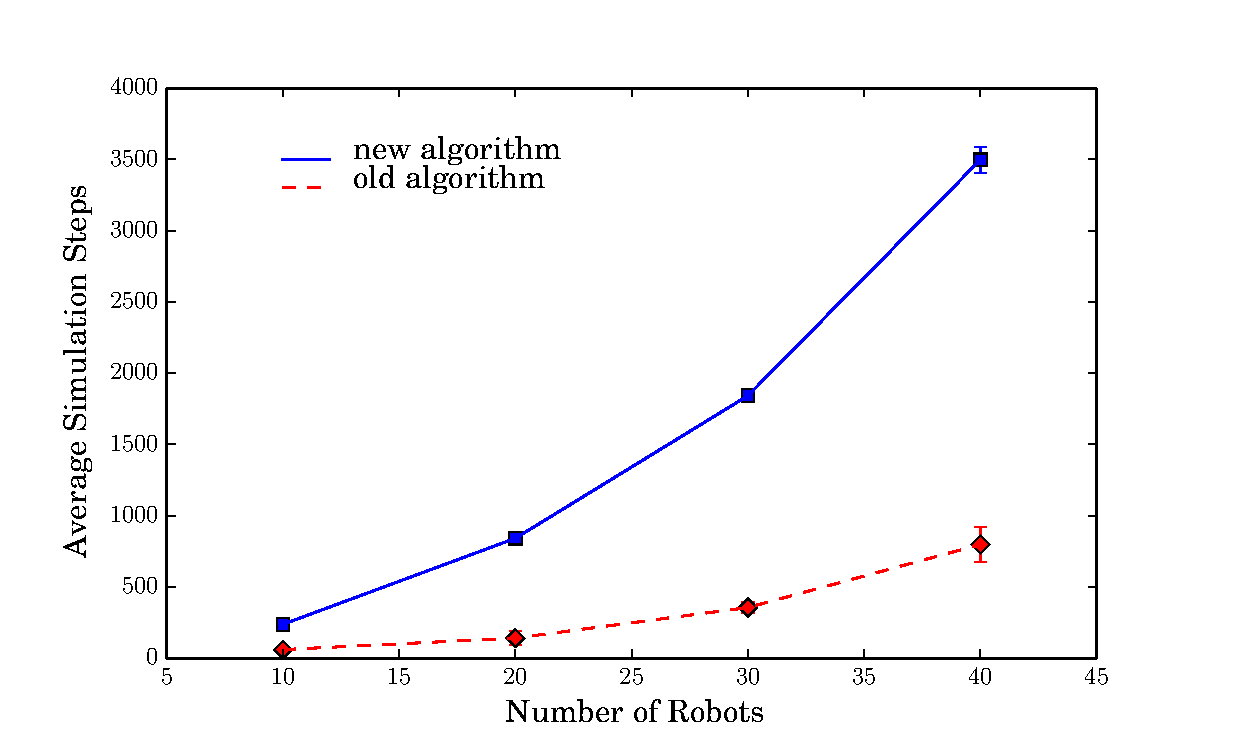
\includegraphics[trim=0.5cm 0cm 1.5cm 0,clip=true,width=\linewidth]{figs/steps_square}
    \end{minipage}
    \begin{minipage}[b]{0.75\linewidth}
    \centering 
      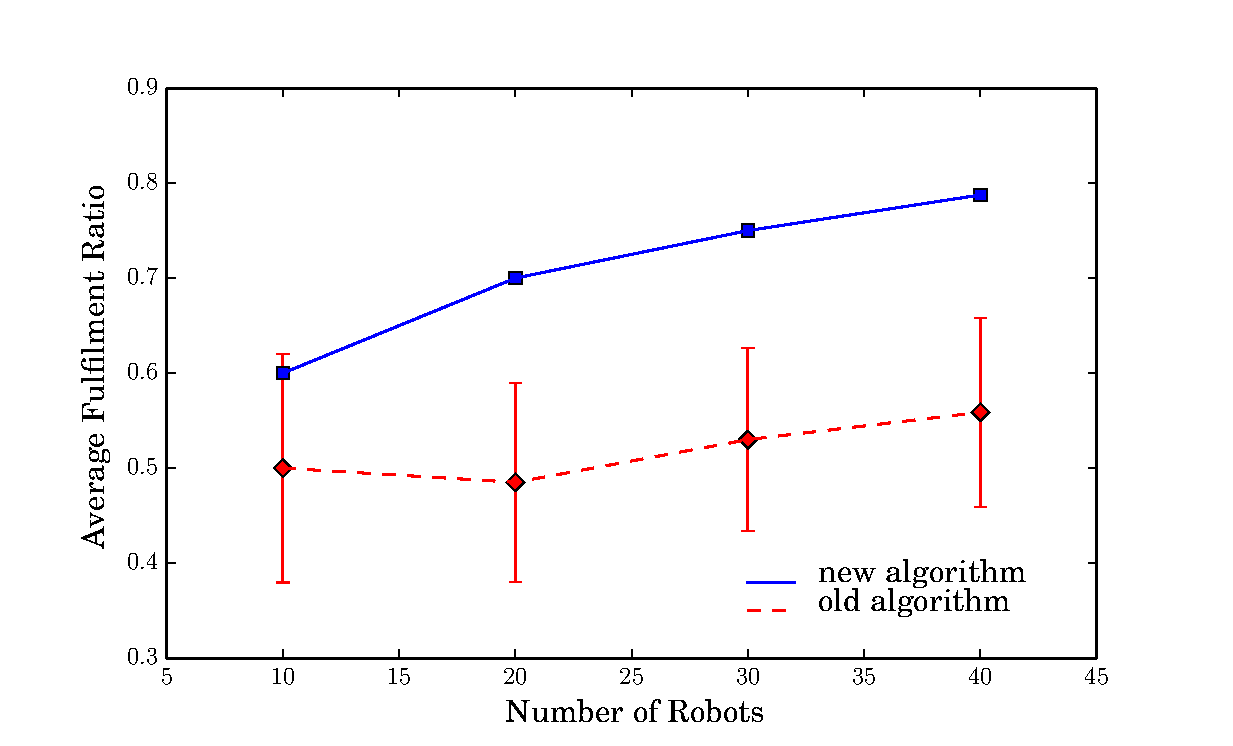
\includegraphics[trim=0.5cm 0 1.5cm 0,clip=true,width=\linewidth]{figs/ratio_square}
    \end{minipage}
    \caption{Repeated squares pattern: [left] The average execution time with deviation. [right] The average fulfillment ratio with deviation.}
    \label{fig:sq_comp}
  \end{figure}
  %%%%%%%%%%%%%%%%%%%%%%%%%%%%%%%%
 %%%%%%%%%%%%%%%%%%%%%%%%%%%%%%%%
  \begin{figure}
  \centering 
    \begin{minipage}[b]{0.75\linewidth}
    \centering 
      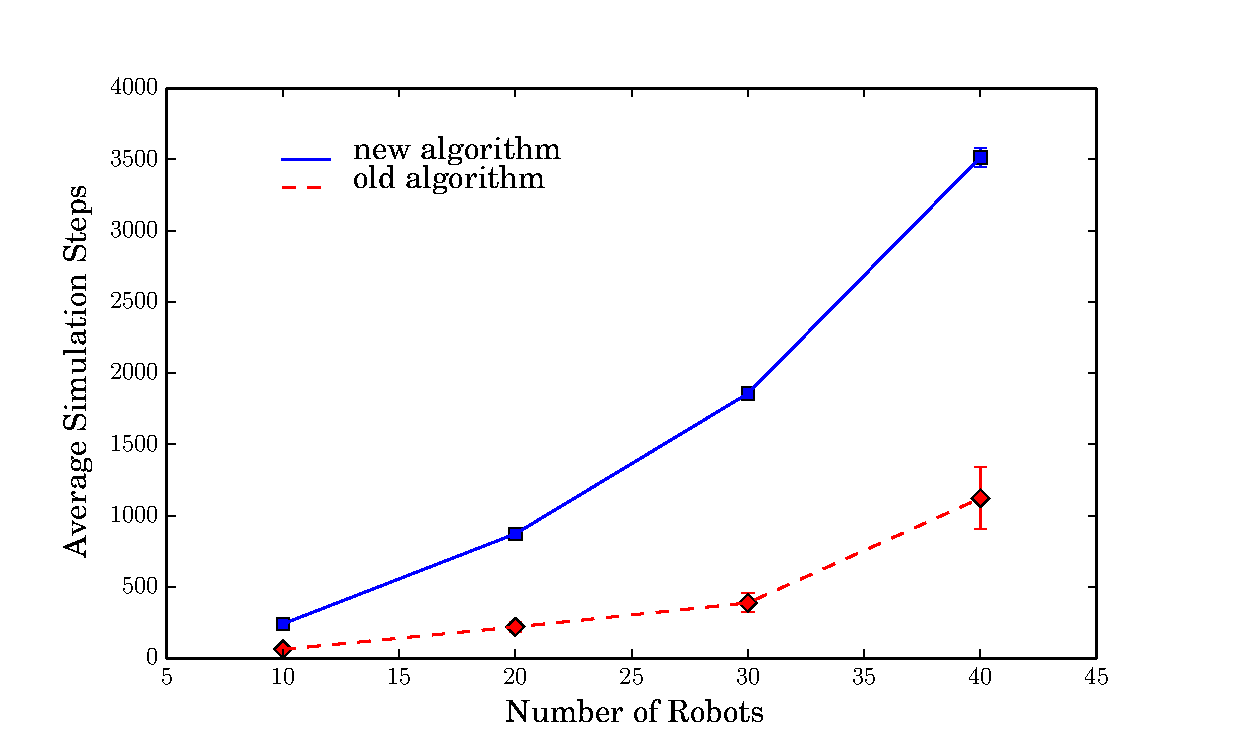
\includegraphics[trim=0.5cm 0cm 1.5cm 0,clip=true,width=\linewidth]{figs/steps_hexagon}
    \end{minipage}
    \begin{minipage}[b]{0.75\linewidth}
    \centering 
      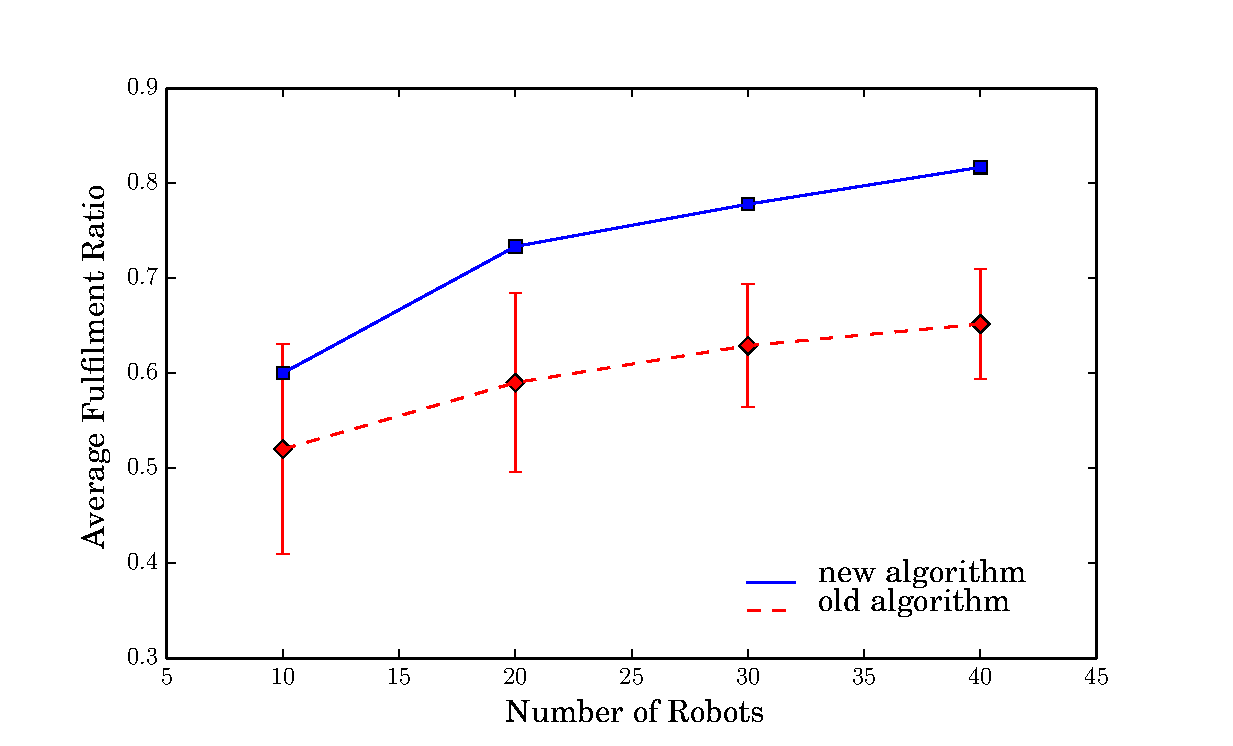
\includegraphics[trim=0.5cm 0 1.5cm 0,clip=true,width=\linewidth]{figs/ratio_hexagon}
    \end{minipage}
    \caption{Repeated hexagons pattern: [left] The average execution time with deviation. [right] The average fulfillment ratio with deviation.}
    \label{fig:hex_comp}
  \end{figure}
  %%%%%%%%%%%%%%%%%%%%%%%%%%%%%%%%
  %%%%%%%%%%%%%%%%%%%%%%%%%%%%%%%% 
  \begin{figure}
  \centering 
    \begin{minipage}[b]{0.75\linewidth}
    \centering 
      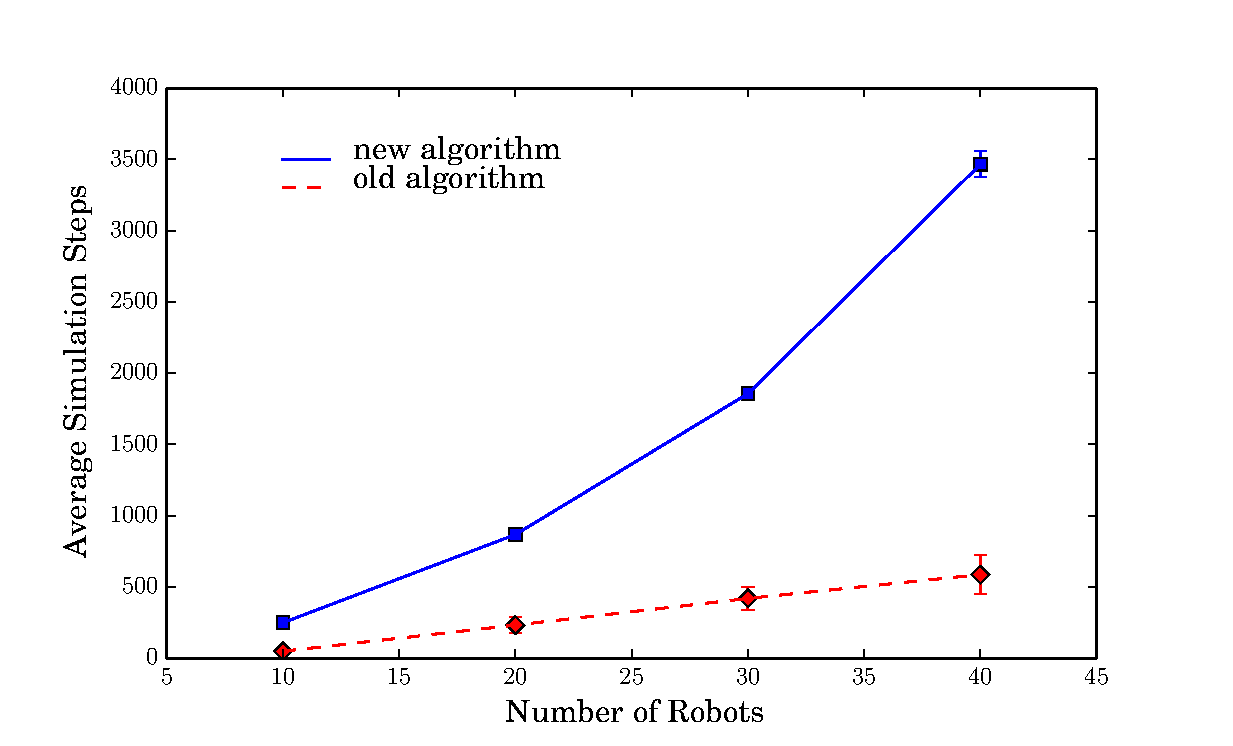
\includegraphics[trim=0.5cm 0cm 1.5cm 0,clip=true,width=\linewidth]{figs/steps_octagon_square}
    \end{minipage}
    \begin{minipage}[b]{0.75\linewidth}
    \centering 
      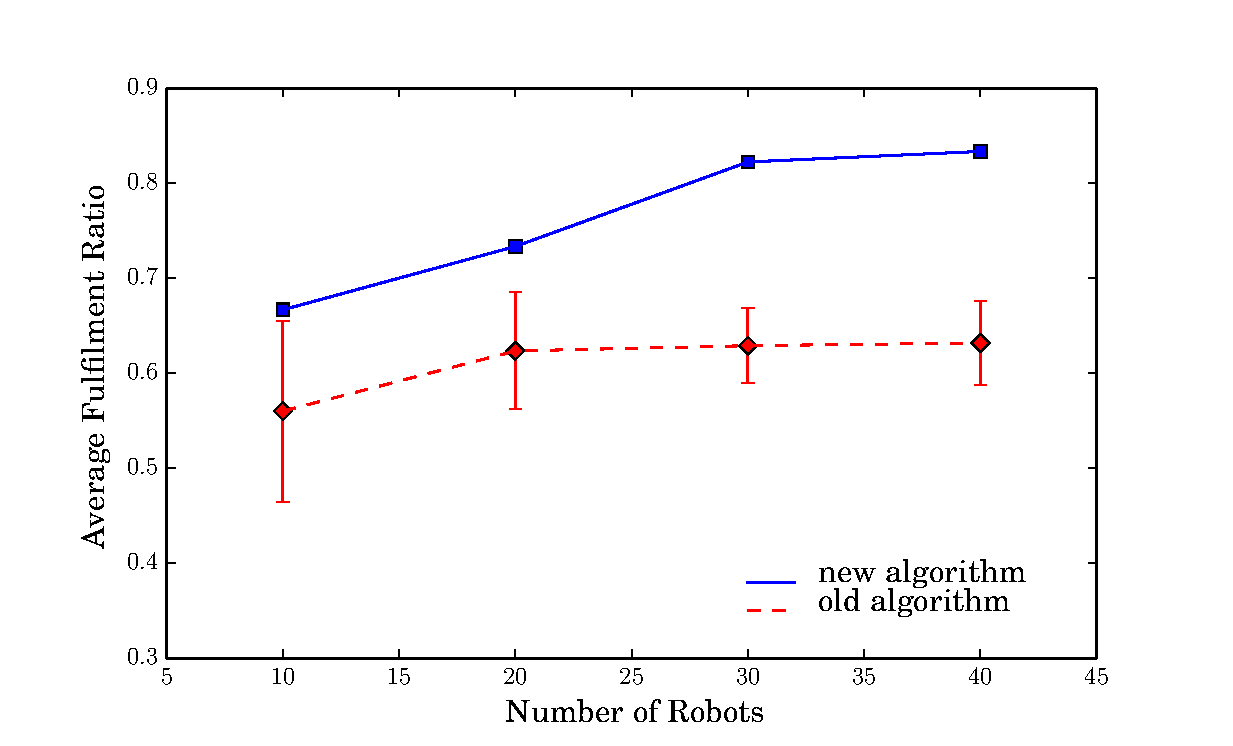
\includegraphics[trim=0.5cm 0 1.5cm 0,clip=true,width=\linewidth]{figs/ratio_octagon_square}
    \end{minipage}
    \caption{Repeated octagons and squares pattern: [left] The average execution time with deviation. [right] The average fulfillment ratio with deviation.}
    \label{fig:octsq_comp}
  \end{figure}
  %%%%%%%%%%%%%%%%%%%%%%%%%%%%%%%%
  
%\clearpage
\section{Discussions}
\label{sec:conc-mrf2}

In this chapter, we have introduced the second type of decentralized formation algorithm for the problem in Chapter~\ref{chp:mrf}.
%
Compared with the method in Chapter~\ref{chp:mrf1}, we conclude that this algorithm is provably-correct in its bounded-time execution and improved formation quality notably.
%
Another feature of this algorithm is the NCLB motion strategy that maintains the connectivity of the communication graph during its execution.


However, there are two major limitations for this approach:
\begin{enumerate}
\item Inefficient performance: each time only one robot moves to a vacancy, and the travel distance of each relocation process is far from optimal.
\item Lack of the robustness and error-tolerance: in contrast to the primary algorithm, the new approach may encounter failures when some robots in the systems fail to work properly. Take Figure~\ref{fig:safedist2} as an example, if robot $r_4$ does not perform message passing or fails to move, then the desired lattice cannot be formed correctly, and the algorithm will never terminate. 
Another scenario is that, when some new robots with IDs higher than any robot's ID join in the system, the algorithm may not response well. 
Consider Figure~\ref{fig:forty_sq_comp}, the bottom figure has shown that forty robots already formed a repeating square pattern. 
If a new robot, whose ID is higher than any other robots, joins in the network, then the robots cannot re-organize themselves because there is no way for those stable robots to reset their status back to unstable.
\end{enumerate}




             %% are in the files 
\chapter{Conclusions}
\label{chp:conc}

In this dissertation, two problems are considered. 
The first one is discussing about the capability of a robot to complete a task, without knowing its true I-states but using an approximation of the exact states.
%
The second problem we are interested in is how to solve a lattice pattern formation problem for the multi-robot systems in a distributed manner. 
%
For the first problem we have presented a geometric planning approach, and for the second problem, we have contributed two decentralized multi-robot formation algorithms.


The first algorithm in Chapter~\ref{chp:cga} contributes to a simple data structure, called double-rectangle range space, to represent a robot's knowledge, subject to the bounded sensing and motion uncertainty. 
%
We claim that this geometric approach can do a better I-state over-approximation job by comparing it with existed approaches. 
%
Hence, this approach provides a robot, that is equipped with extremely limited sensing and motion units, a high success rate to complete many landmark-based navigation tasks.
%
Additionally, we argue that the extensibility of this approach, that is, the idea of ``k-fold unions of rectangle range spaces'' is useful for more accurate I-state over-approximation with a certain level sacrificing of the computation efficiency.
%
We realize that there may some future work to think about. 
For example, the geometric approach to
generate \emph{under}-approximation of the I-states.  
%
The discrepancy between the over- and under-approximations could then be used by the robot to estimate the quality of its representation.

We have presented two novel decentralized methods to solve the multi-robot lattice formation problem in Chapter~\ref{chp:mrf1} and Chapter~\ref{chp:mrf2}, respectively. 
%
The major challenge is the constraint of using only robots' local information to form various lattice pattern.  

To let the algorithm be generally useful for constituting various lattice patterns, rather than solving only one pattern formation problem, we have created a graph representation of the desired pattern.
%
Both of our formation algorithms use the graph representation as input.


To overcome the local information constraint, the first formation algorithm uses a distributed task assignment strategy to form local pattern. 
%
It also uses a collection of authority trees to organize robots into a global structure.
%
In contrast, the second formation algorithm uses scheduling-like strategy to complete the desired pattern by sequentially relocating one robot to an open vacancy that constitutes a part of the lattice. 
%
The key features of the second formation algorithm also include the spanning tree construction and the ``No Child Left Behind'' motion strategy that maintains the connectivity of the communication graph during the algorithm execution.

It is difficult for us to provide an estimation of time consumption for the task-assignment-based formation algorithm because of the nondeterministic deconstructions of the authority trees. 
%
However, we have proved that the second formation algorithm provides an upper-bound of the execution time for robots to form desired lattice patterns.  
%
That is, the algorithm execution time is generally bounded by a value quadratic to the number of robots ($O(n^2)$) only, regardless of the lattice pattern to constitute.


We realize currently the second formation algorithm is not efficient and robust enough,  but it has a great potential to expand itself. 
%
In current version there is only one robot relocating to one vacancy at a time. 
%
We anticipate to expand the algorithm so that multiple robots could be
relocated to multiple vacancies at a time. 
%
Particularly, we expect to construct $k, 1\leq k < n$ spanning trees from the communication graph, by finding the $k$ highest ID stable robots with vacancies,
and $k$ highest ID unstable robots in the system.
Thus, the major challenge becomes: how to design a proper motion strategy to enable multiple robots make progress to their goals, while maintaining the connectivity of the communication graph?
%
Furthermore, to enhance the the algorithm's robustness to the robots failures, we are also interested in designing an error-tolerance mechanism such that a robot can recover from an error status.
% \include{Hypercubes}	   %% Cubes.tex and Hypercubes.tex
       
                           
% \include{1mod4}
% \include{flying}
% \include{joins}
% \include{wattage}

% \include{3mod4}	          %% This chapter has 8 sections
% \include{bigtime}         %% You should give your sections
% \include{smalltime}       %% logical names, rather than
% \include{roadmap}         %% numbers. As you write, you might
% \include{overview}        %% decide to rearrange things. 
% \include{turnabout}       %% LaTeX can keep track of the
% \include{fairplay}        %% numbering for you.
% \include{roundup}

% \include{rest}
% \include{relax}
% \include{grin}

%\include{Conclusion}     %% Honors theses are required to 
                          %% have an unnumbered chapter
                          %% for conclusions.  The file
                          %% Conclusion.tex should begin
                          %%   
                          %% \chapter*{Conclusion}
                          %% followed by the appropriate
                          %% text.

\printbibliography %%  This is the command to use to
			       %%  insert the bibliography if you are using
                           %% the biblatex.sty package.  See the 
                           %% uscthesisdoc.pdf documentation for
                           %% for alternative bibliographic systems.     

%\Appendix                 %% Use this command if you have one 
                          %% appendix. Use \Appendices if you 
                          %% have more than one.
	
%\input{toolong}         %% Calls toolong.tex which contains
                          %% an appendix. After issuing the 
                        %% command \Appendix or \Appendices
                        %% you must use \input not \include
                        %% to load the first appendix.

\end{document}
%%%%%%%%%%%%%%%%%%%%%%%%%%%%%%%%%%%%%%%%%%%%%%%%%%%%%%%%%%%%%%%